\documentclass[12pt]{beamer}

\newcommand{\emp}{\noindent\fboxsep=0pt}
\usefonttheme{serif}

\usetheme{Darmstadt}
\usepackage[utf8]{inputenc}
\usepackage[UTF8,zihao=-4]{ctexcap}
\usepackage[T1]{fontenc}
\usepackage{lmodern}
\usepackage{wrapfig}
\usepackage{fontspec}
\usepackage{color}
\usepackage{fancyhdr}
\usepackage{setspace}
\usepackage{caption}
\usepackage{mathptmx}
\usepackage{amsmath}
\usepackage{amssymb}
\usepackage{amstext}
\usepackage{geometry}
\usepackage{graphicx}
\usepackage{pifont}
\usepackage{float}
\usepackage{newclude}
\usepackage{subfig}
\usepackage{paralist}
\usepackage{booktabs} % 允许在表中使用\toprule、\ midrule和\ bottomrule% 定义正文字体
\usepackage[bookmarks=true]{hyperref}
\usepackage{tabularx}
%\usepackage{listings}


\setromanfont{Times New Roman}	% 将西文字体设置为 Times New Roman
% \setCJKfamilyfont{zhkai}{[SIMKAI.TTF]}
% \newcommand*{\kaiti}{\CJKfamily{zhkai}}

% 定义 caption
\DeclareCaptionFont{kaiticaption}{\kaishu \small}	% 定义下面三个caption的font的kaiticaption的具体格式
\captionsetup[figure]{font=small,labelsep=quad,skip=0.5ex,labelfont=bf,font=kaiticaption}	% 设置图片的 caption 格式 % 想要标题换行后居中,可以添加justification=centering
\captionsetup[table]{font=small,labelsep=quad,skip=0.5ex,labelfont=bf,font=kaiticaption}	% 设置表格的 caption 格式
\captionsetup[subfloat]{font=small,labelsep=quad,skip=0.5ex,labelfont=bf,font=kaiticaption}
\captionsetup[equation]{font=small,labelsep=quad,skip=0.5ex,labelfont=bf,font=kaiticaption}


% 设置图片,表格,公式编号格式
\renewcommand{\thetable}{\thesection{}-\arabic{table}}	% \thetable 表示设置的是表格的编号格式, 后面括号的内容为编号格式:章节号-表格的序号
\renewcommand{\thefigure}{\thesection{}-\arabic{figure}}
\renewcommand{\theequation}{\thesection{}-\arabic{equation}}


% 设置代码块
%\definecolor{commentcolor}{RGB}{85,139,78}
%\definecolor{stringcolor}{RGB}{206,145,108}
%\definecolor{keywordcolor}{RGB}{34,34,250}
%\lstset{
%	language=Matlab, % 默认代码语言.
%	basicstyle=\footnotesize,
%	numbers=left, %设置行号位置
%	numberstyle=\tiny, %设置行号大小
%	commentstyle=\color{commentcolor},	%注释颜色
%	keywordstyle=\color{keywordcolor},	%关键词颜色
%	stringstyle=\color{stringcolor},	%字符串颜色
%	frame=single, %设置边框格式
%	escapeinside=``, %逃逸字符(1左面的键),用于显示中文
%	breaklines = True, % 自动折行
%	breakatwhitespace = True, % 自动折行时打断单词
%	extendedchars=false, %解决代码跨页时,章节标题,页眉等汉字不显示的问题
%	xleftmargin=2em,xrightmargin=2em, aboveskip=1em, %设置边距
%	tabsize=4, %设置tab空格数
%	showspaces=false %不显示空格
%}

\graphicspath{{../img/}}
% 下面两行用于删除导航栏
\useoutertheme{split}
\setbeamertemplate{headline}{}
\newcommand\struc[3][]{\begin{frame}
		\begin{block}{#1}
			\begin{compactitem}
				\item structure
					\begin{figure}[htbp]
						\centering
						\includegraphics[width=#2\textwidth]{#3}
					\end{figure}
\end{compactitem}
\end{block}
\end{frame}}

\begin{document}
\abovedisplayshortskip=0pt	%设置公式距离上方非重叠区域额外添加的距离,推荐0
\belowdisplayshortskip=0pt
\abovedisplayskip=0pt	%设置公式距离上方重叠距离额外添加的距离,推荐0
\belowdisplayskip=0pt
\section{Power System}
\begin{frame}
	\centering\Huge\textbf{Power System}
\end{frame}
% 当前subsection第一页
\subsection{Engine Overview}
\begin{frame}{Engine Overview}	% 括号里填subsection
	\begin{block}{} % subsubsection
		\begin{figure}[htbp]
			\centering
			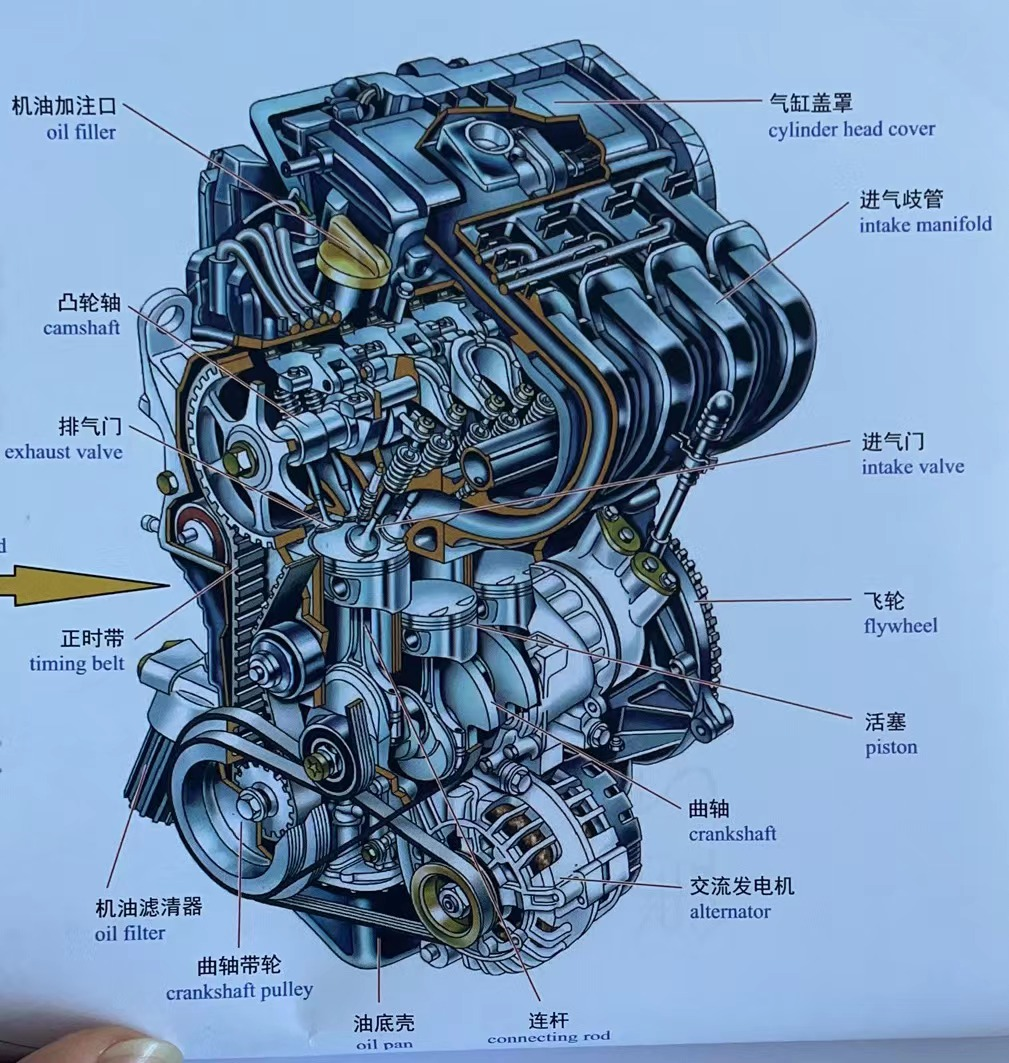
\includegraphics[width=0.6\textwidth]{2-1}
		\end{figure}
	\end{block}
\end{frame}
\subsection{Engine Types}
\begin{frame}{Engine Types}	% 当前subsection的第二页
	\begin{block}{Gasoline Engine}
		mainly for passenger car
		\begin{figure}[htbp]
			\centering
			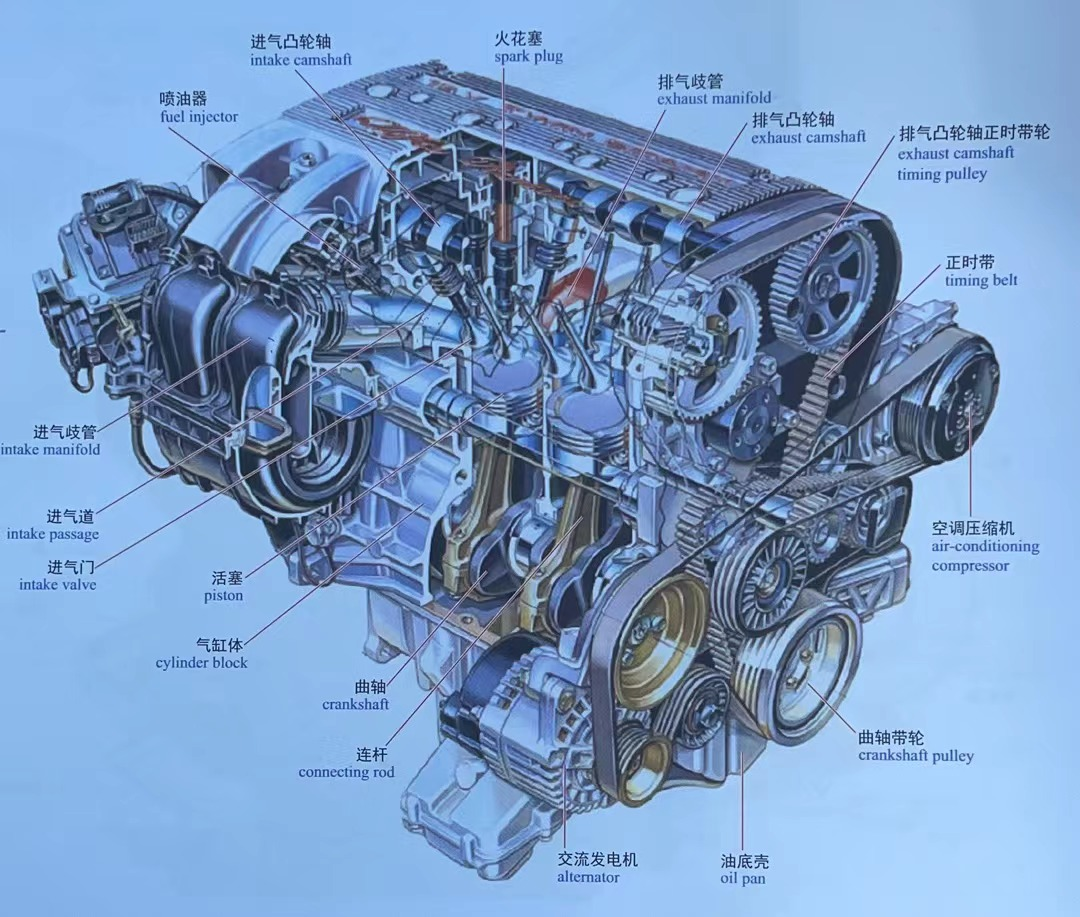
\includegraphics[width=0.6\textwidth]{2-2}
		\end{figure}
	\end{block}
\end{frame}
\begin{frame}
	\begin{block}{Diesel Engine}
		\begin{figure}[htbp]
			\centering
			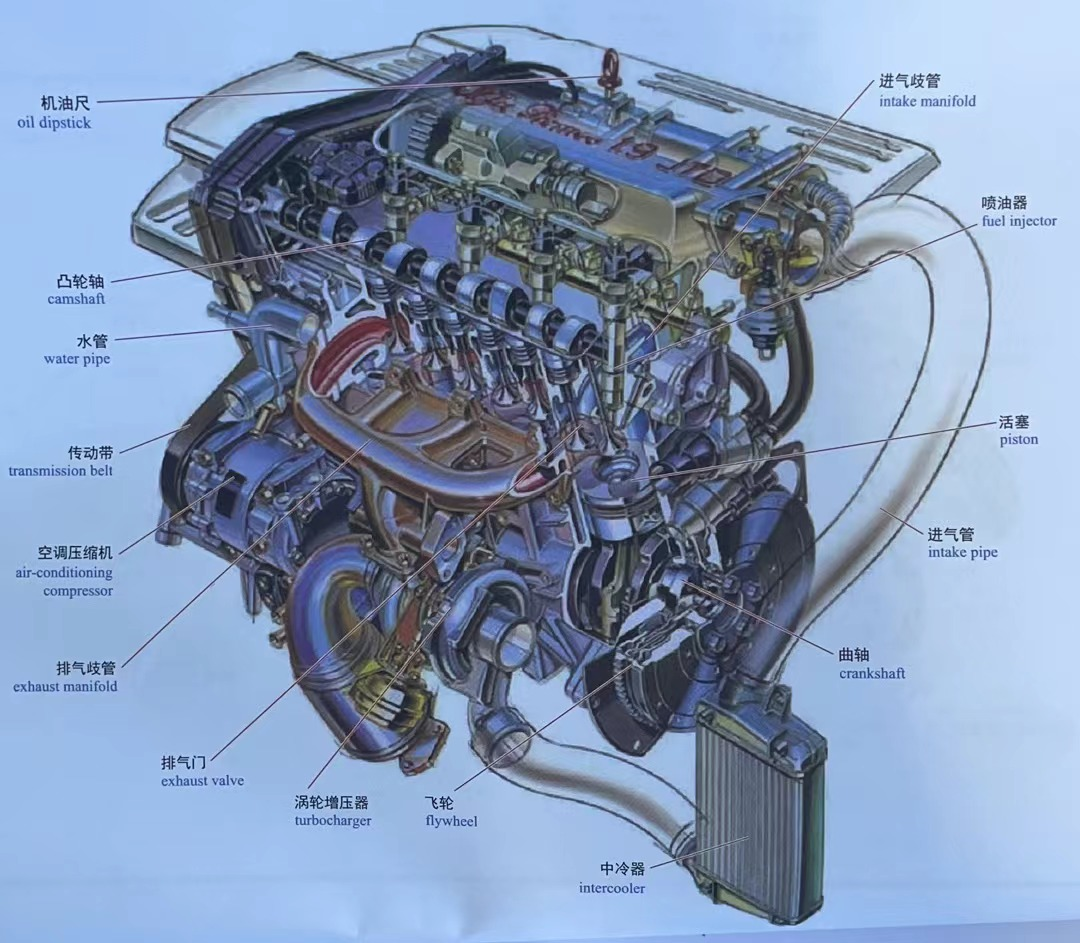
\includegraphics[width=0.8\textwidth]{2-3}
		\end{figure}
	\end{block}
\end{frame}
\begin{frame}
	\begin{block}{Rotary Engine}
		\begin{figure}[htbp]
			\centering
			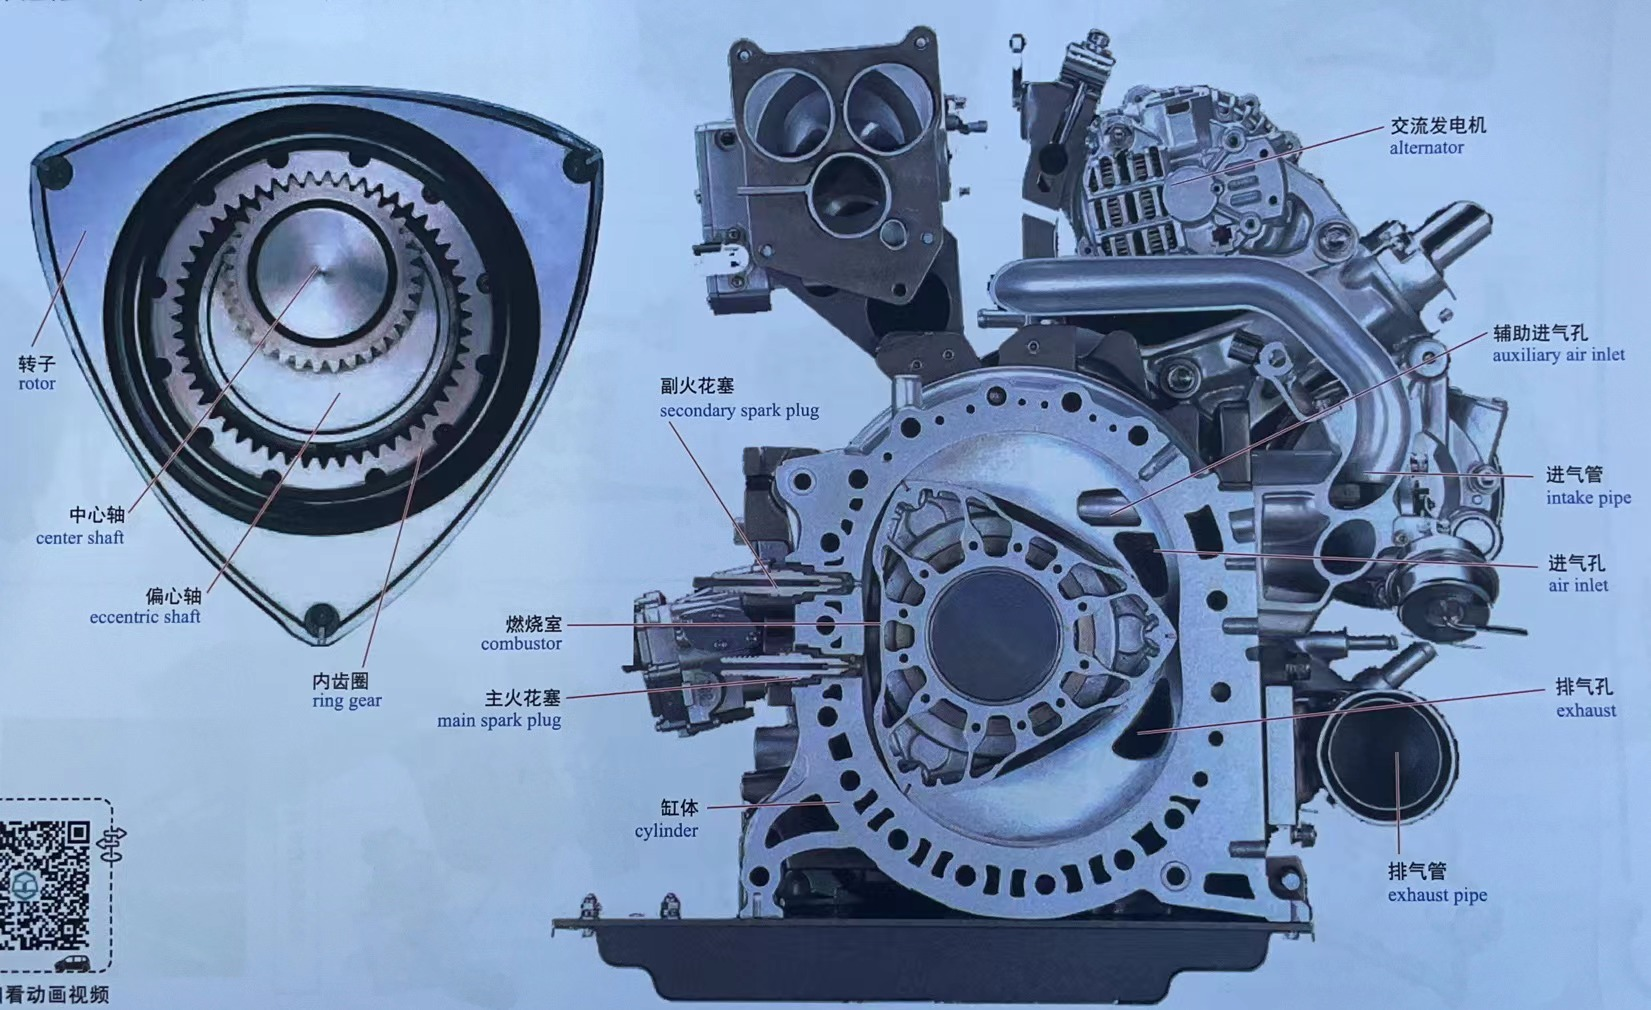
\includegraphics[width=0.8\textwidth]{2-4}
		\end{figure}
	\end{block}
\end{frame}

\subsection{Engine Components Overview}
\begin{frame}{Engine Components Overview}
	A gasoline engine is usually composed of 2 mechanisms and 5 systems.
	\begin{equation*}
		mechanisms =
			\begin{cases}
				\text{connecting rod mechanisms} \\
				\text{valve train mechanisms}
			\end{cases}
	\end{equation*}
	\begin{equation*}
		systems =
			\begin{cases}
				\text{fuel supply system} \\
				\text{ignition system} \\
				\text{starting system} \\
				\text{lubrication system} \\
				\text{cooling system}
			\end{cases}
	\end{equation*}
\end{frame}
\begin{frame}
	A diesel engine is usually composed of 3 mechanisms and 4 systems
	\begin{equation*}
		mechanisms =
		\begin{cases}
			\text{connecting rod mechanisms} \\
			\text{valve train mechanisms}\\
			\text{drive mechanisms}
		\end{cases}
	\end{equation*}
	\begin{equation*}
		systems =
		\begin{cases}
			\text{fuel supply system} \\
			\text{starting system} \\
			\text{lubrication system} \\
			\text{cooling system}
		\end{cases}
	\end{equation*}
\end{frame}
\begin{frame}
	\begin{block}{connecting rod mechanism}
		\begin{compactitem}
			\item 
			$
				\text{components} = \begin{cases}
					\text{body group} \\
					\text{piston connecting rod set} \\
					\text{crankshaft flywheel set}
				\end{cases}
			$
			\item function : the main part for the engine that realizes the working cycle and energy conversion
		\end{compactitem}
	\end{block}
\end{frame}
\begin{frame}
	\begin{block}{valve train mechanisms}
		\begin{compactitem}
			\item
				$
				\text{components} = \begin{cases}
					\text{valve group} \\
					\text{drive group}
				\end{cases}
				$
			\item function: regularly open and close valves, letting air and combustible mixture enter the cylinder and exhausting waste gas.
		\end{compactitem}
	\end{block}
\end{frame}
\begin{frame}
	\begin{block}{}
		\begin{compactitem}
			\item structure
				\begin{figure}[htbp]
					\centering
					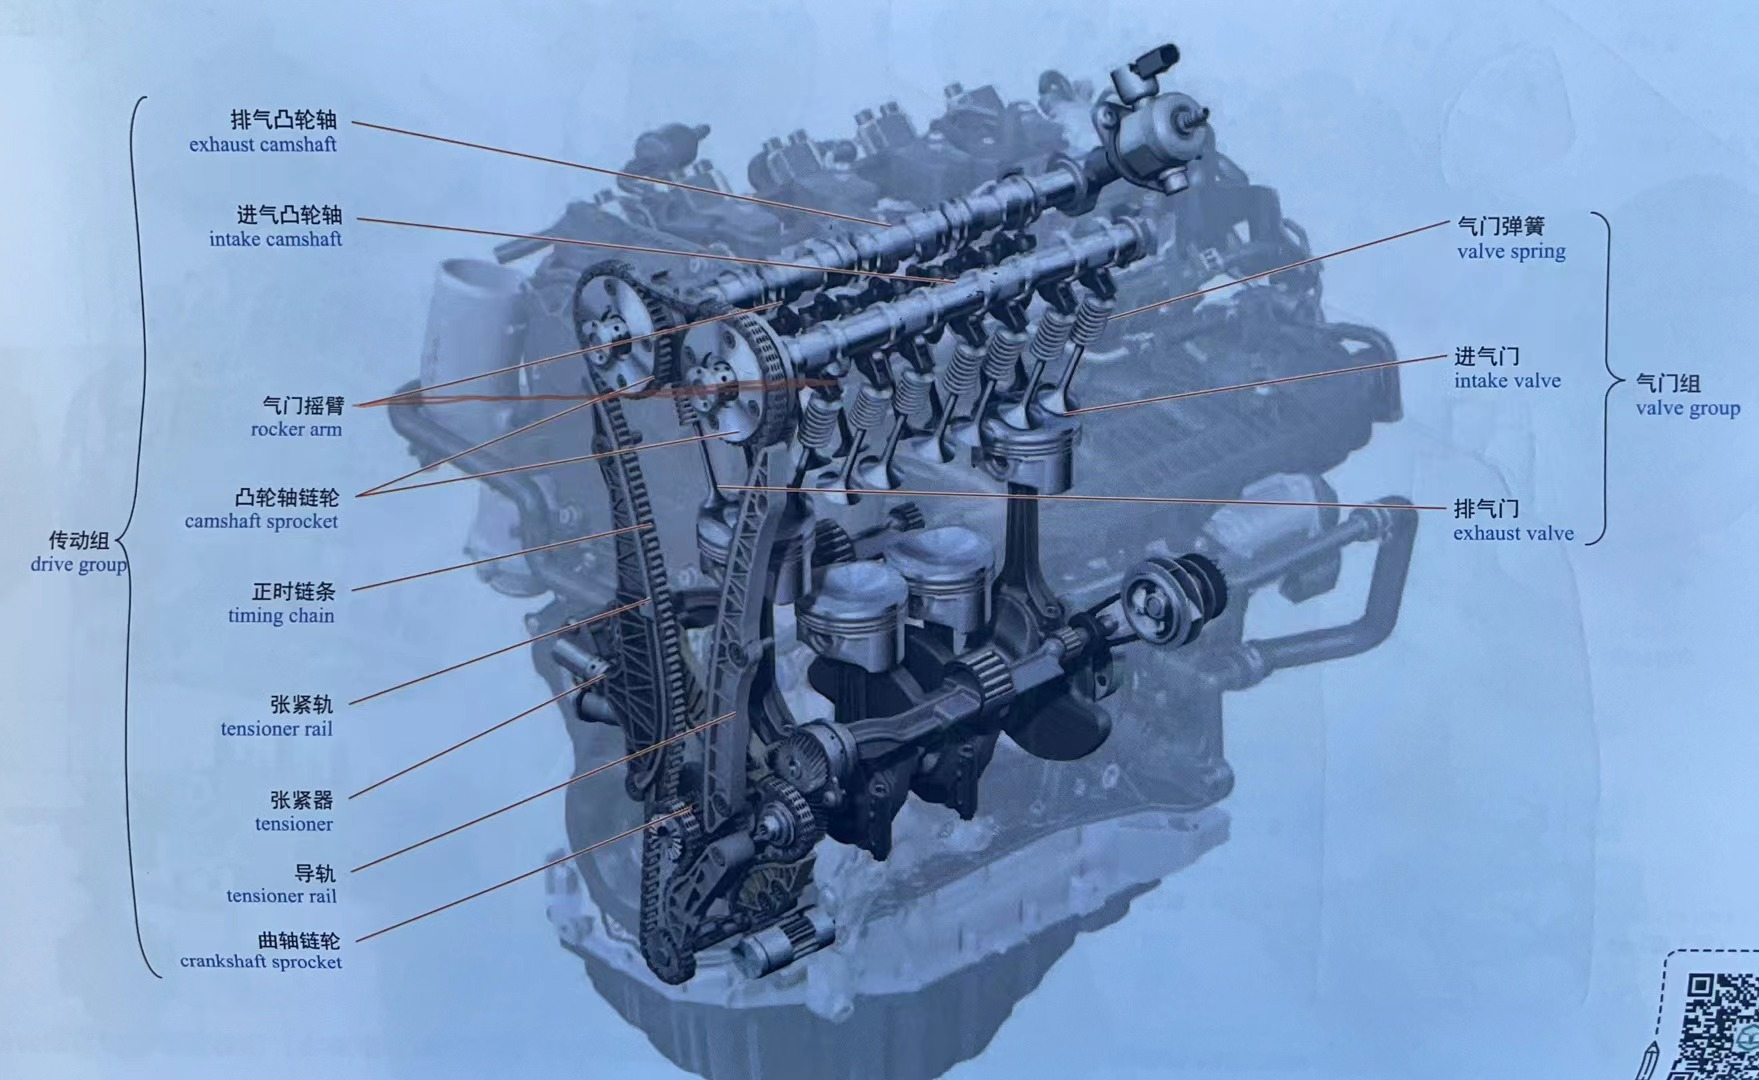
\includegraphics[width=0.8\textwidth]{2-6}
				\end{figure}
		\end{compactitem}
	\end{block}
\end{frame}
\begin{frame}
	\begin{block}{fuel system}
		\begin{compactitem}
			\item function: prepare a certain proportion of the air-fuel mixture/directly inject the fuel into the cylinder to mix with the compressed air
			\item structure
				\begin{figure}[htbp]
					\centering
					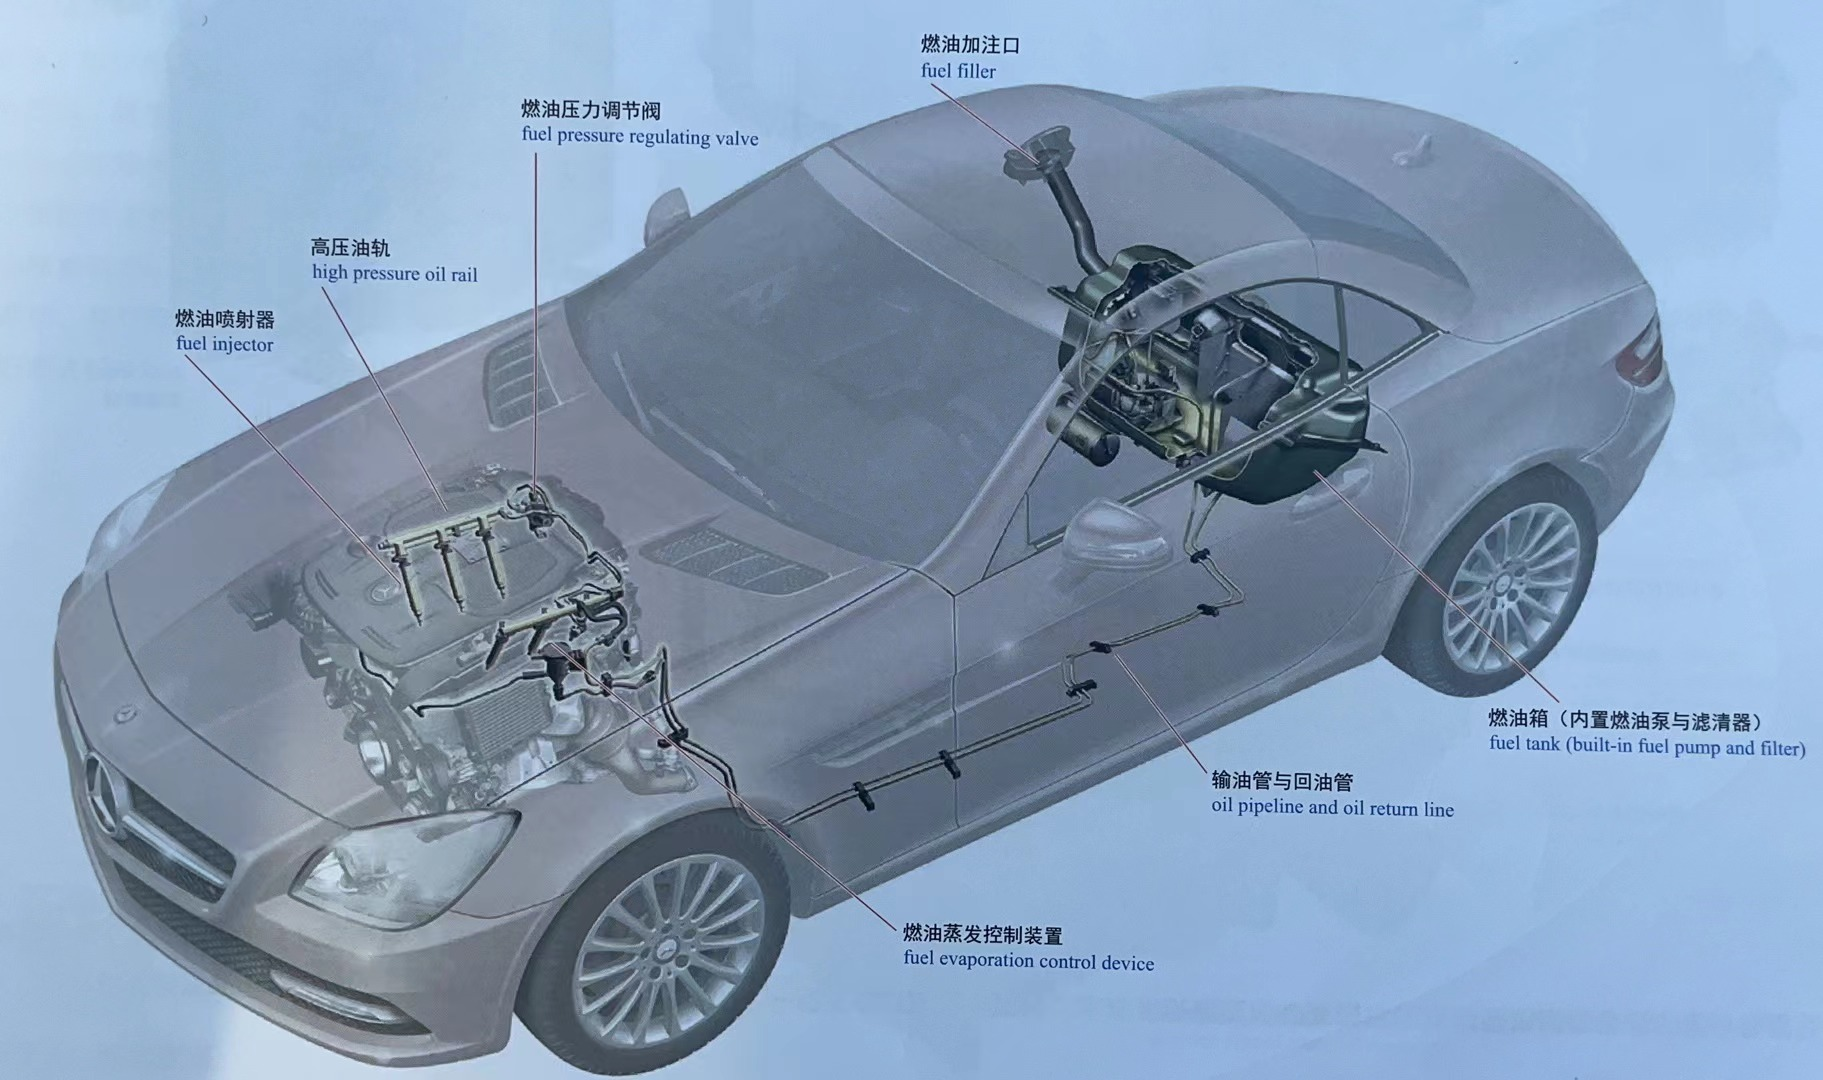
\includegraphics[width=0.8\textwidth]{2-7}
				\end{figure}
		\end{compactitem}
	\end{block}
\end{frame}
\begin{frame}
	\begin{block}{cooling system}
		\begin{figure}[htbp]
			\centering
			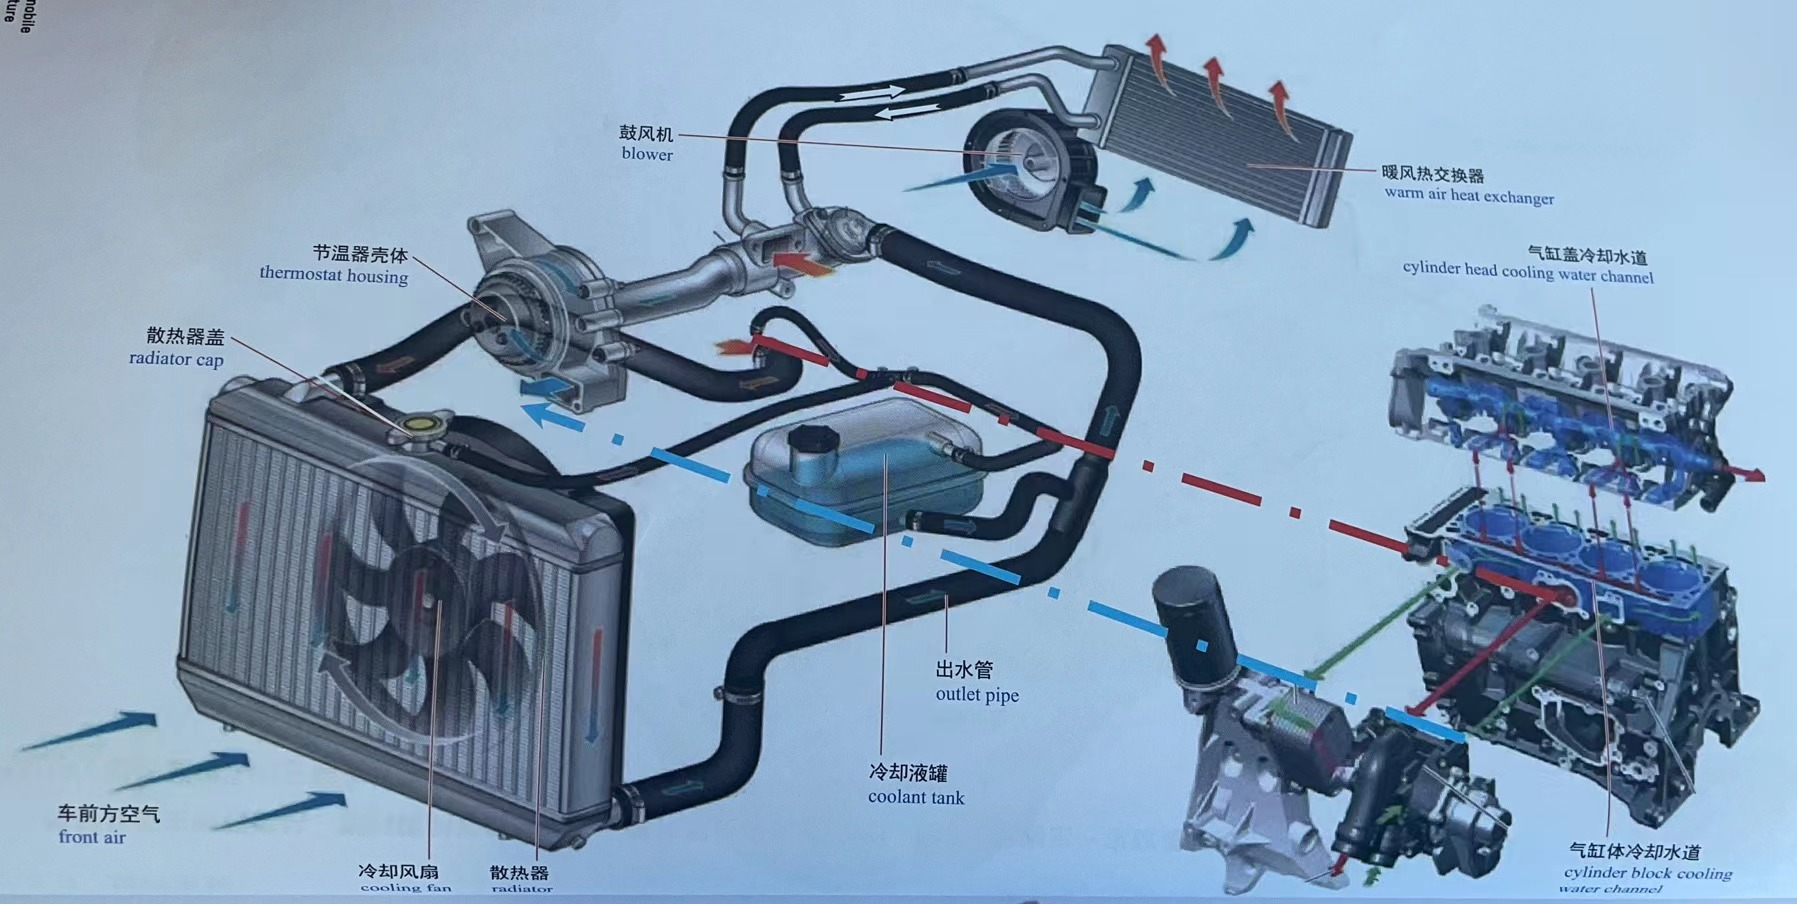
\includegraphics[width=0.7\textwidth]{2-11}
		\end{figure}
	\end{block}
\end{frame}
\begin{frame}
	\begin{block}{lubrication system}
		\begin{figure}[htbp]
			\centering
			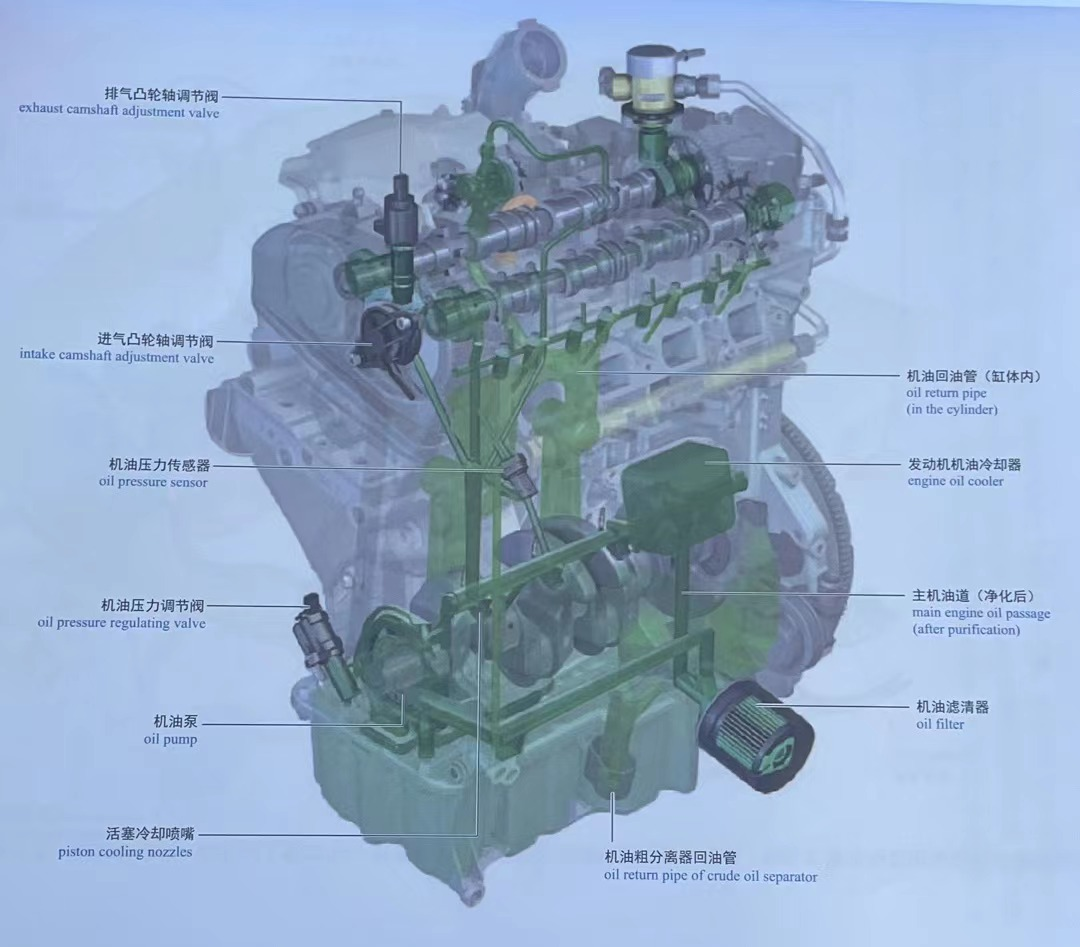
\includegraphics[width=0.7\textwidth]{2-8}
		\end{figure}
	\end{block}
\end{frame}
\begin{frame}
	\begin{block}{starting system}
		\begin{compactitem}
			\item function: $ \text{battery} \xrightarrow{\text{electricity}} \text{starter} \xrightarrow{E_\text{mechanism}} \text{engine}$
			\item structure:
				\begin{figure}[htbp]
					\centering
					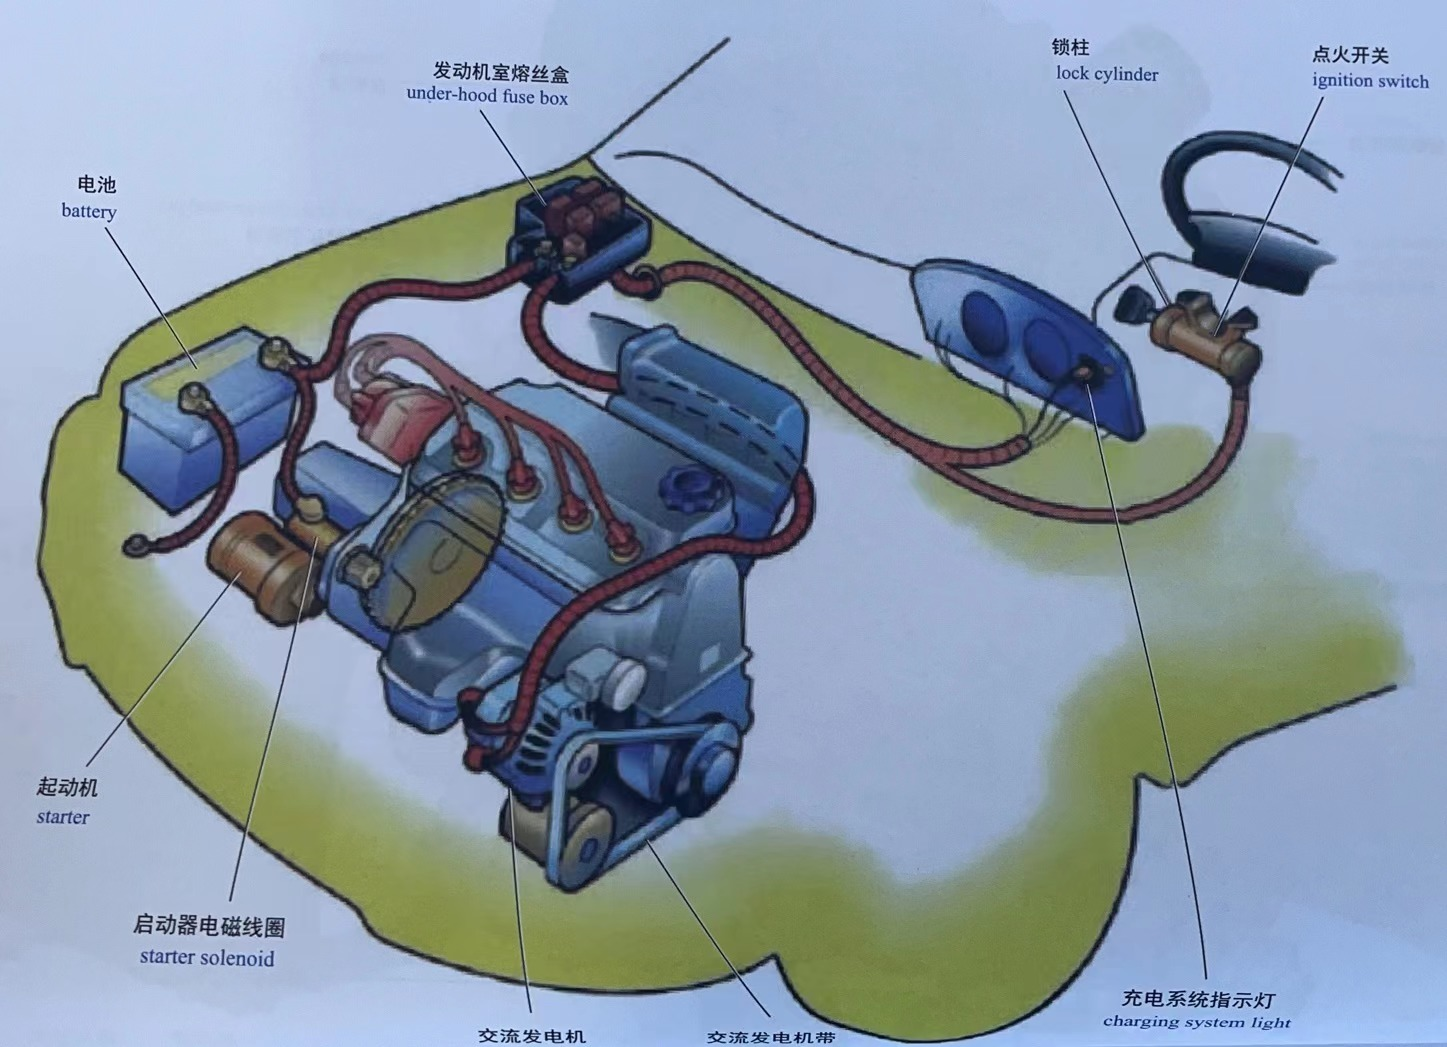
\includegraphics[width=0.7\textwidth]{2-9}
				\end{figure}
		\end{compactitem}
	\end{block}
\end{frame}
\begin{frame}
	\begin{block}{ignition system}
		\begin{figure}[htbp]
			\centering
			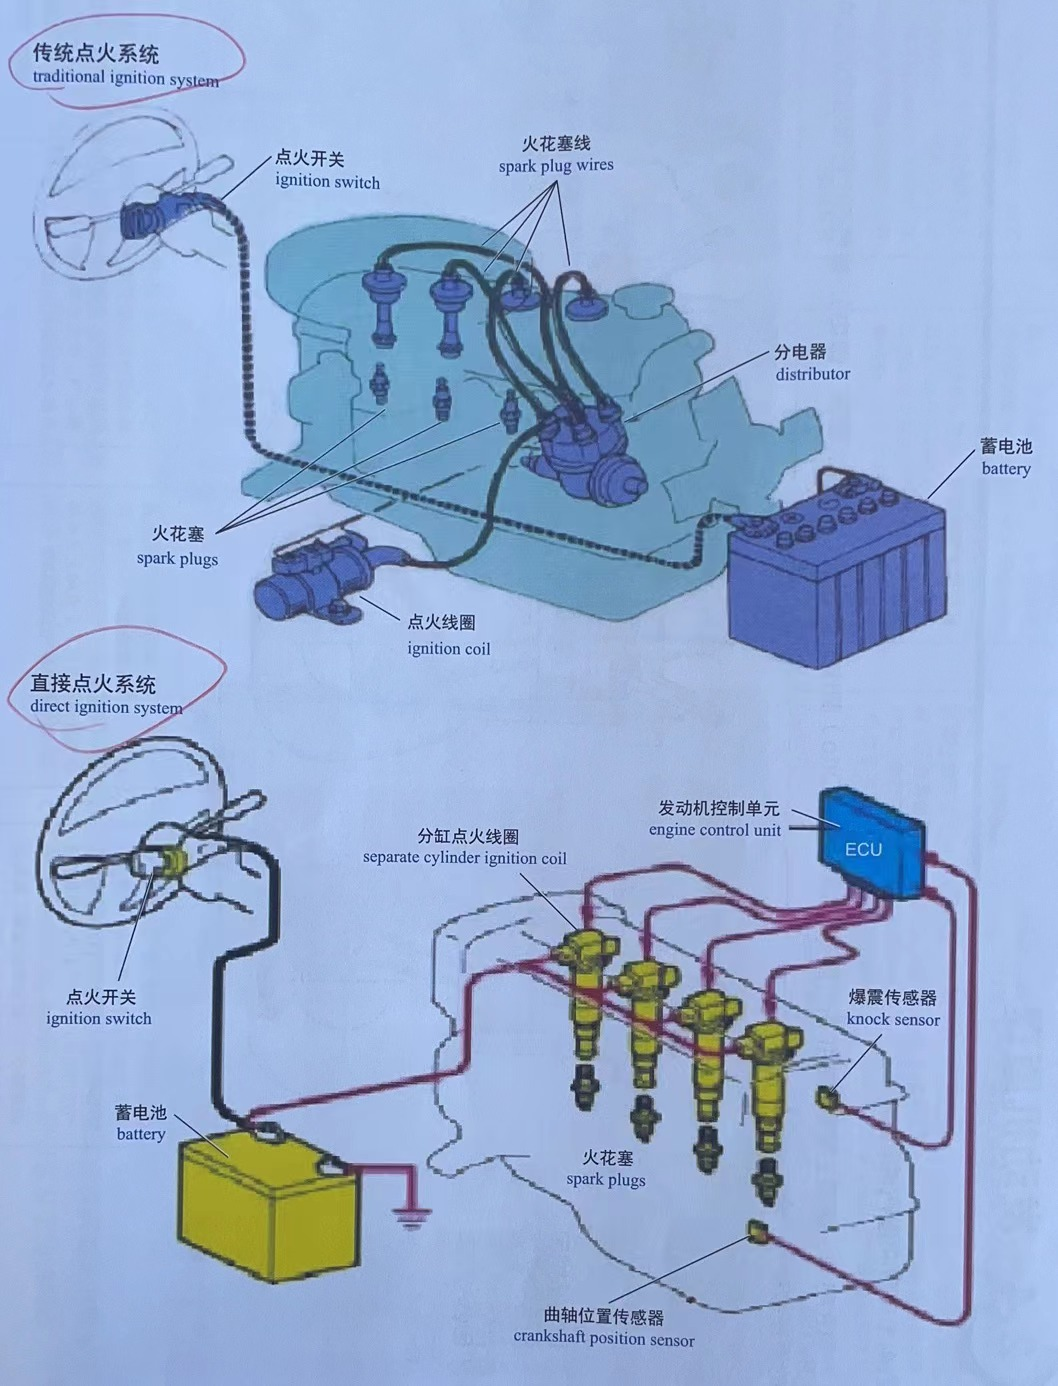
\includegraphics[width=0.5\textwidth]{2-10}
		\end{figure}
	\end{block}
\end{frame}
\subsection{Engine Terms}
\begin{frame}{Engine Terms}
	\begin{block}{terms}
		\begin{compactitem}
			\item TDC(top dead center): the highest position a piston can reach in a cylinder
			\item BDC(bottom dead center)
			\item piston stroke: the distance between the TDC and the BDC
			\item connecting rod length \& crankshaft radius
				\begin{figure}[htbp]
					\centering
					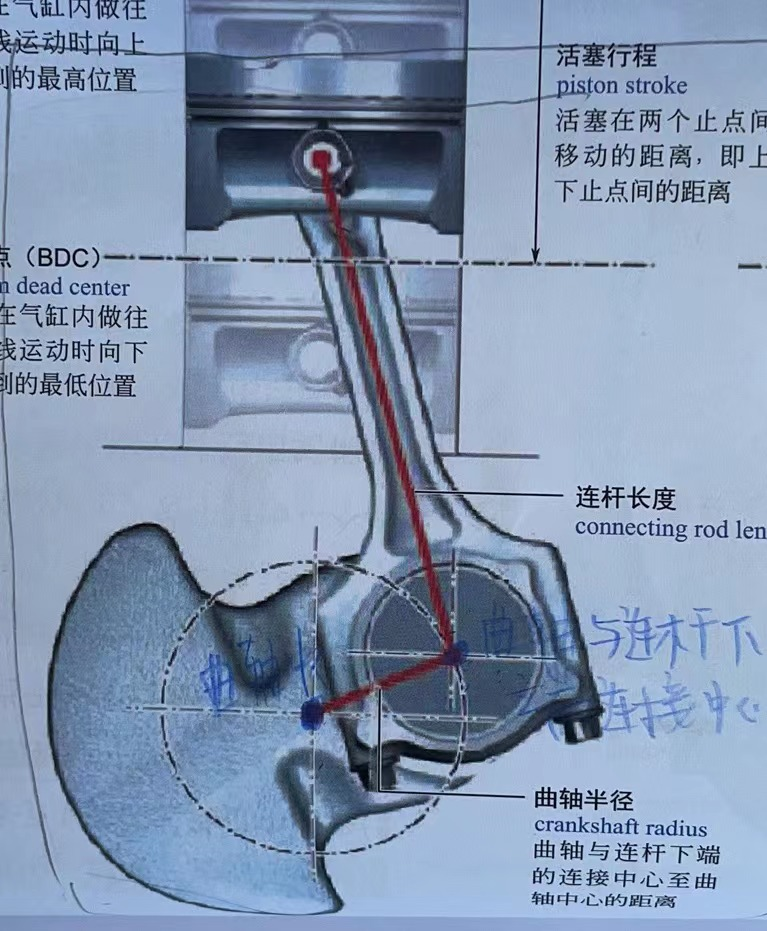
\includegraphics[width=0.3\textwidth]{2-12}
				\end{figure}
		\end{compactitem}
	\end{block}
\end{frame}
\begin{frame}
	\begin{block}{}
		\begin{compactitem}
			\item bore
			\item displacement: the total working volume of each cylinder
			\item combustion chamber volume: the cylinder volume when the piston reaches the TDC
			\item total cylinder volume: the volume between the piston top head and the cylinder cap when the piston reaches the BDC
			\item compression chamber volume: $ V_{cylinder} - V_{compression\ chamber} $
			\item compression ratio: the degree to which the combustible mixture is compressed
				\begin{compactenum}
					\item $ \varepsilon = \dfrac{V_{compression\ chamber} - displacement}{V_{compression\ chamber}}$
					\item low $\varepsilon$ < 10, high $\varepsilon$ > 10
					\item $ \varepsilon \uparrow, power \uparrow $
				\end{compactenum}
			\item power : 1 horse power = 0.746 Kw
		\end{compactitem}
	\end{block}
\end{frame}
\begin{frame}
	\begin{block}{}
		\begin{compactitem}
			\item torque(Nm):
				\begin{compactenum}
					\item torque $\uparrow$, instantaneous acceleration capability $\uparrow$
					\item For a naturally aspirated engine, rotation speed $\uparrow$, torque first $\uparrow$ and then $\downarrow$
					\item For a electric motor, before base speed, n $\uparrow$ power $\uparrow$ torque -; after base speed, n $\uparrow$ power- torque$\downarrow$
				\end{compactenum}
		\end{compactitem}
	\end{block}
\end{frame}
\subsection{connecting rod mechanisms}
\begin{frame}{connecting rod mechanisms}
	\begin{block}{body group}
		\begin{columns}
			\begin{column}{0.4\textwidth}
					components
					\begin{compactitem}
						\item cylinder head cover
						\item cylinder head
						\item cylinder block
						\item cylinder gasket
						\item oil pan
					\end{compactitem}
			\end{column}
			\begin{column}{0.45\textwidth}
					\centering
					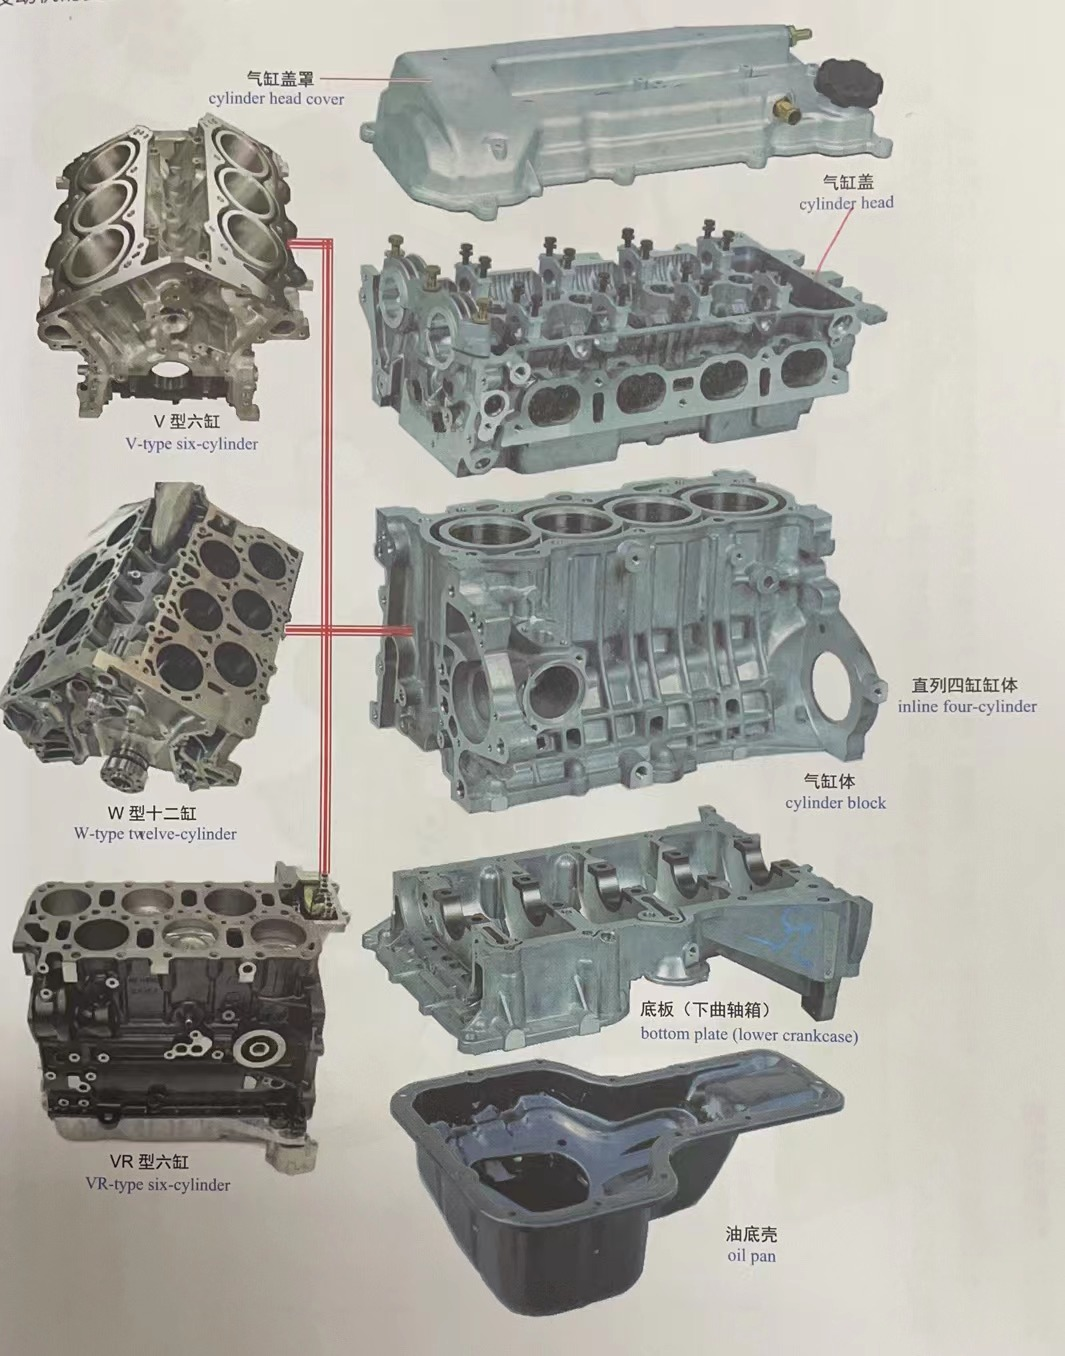
\includegraphics[width=0.95\textwidth]{2-13}
			\end{column}
		\end{columns}
	\end{block}
\end{frame}
\begin{frame}
	\begin{block}{piston connecting rod group}
		\begin{center}
			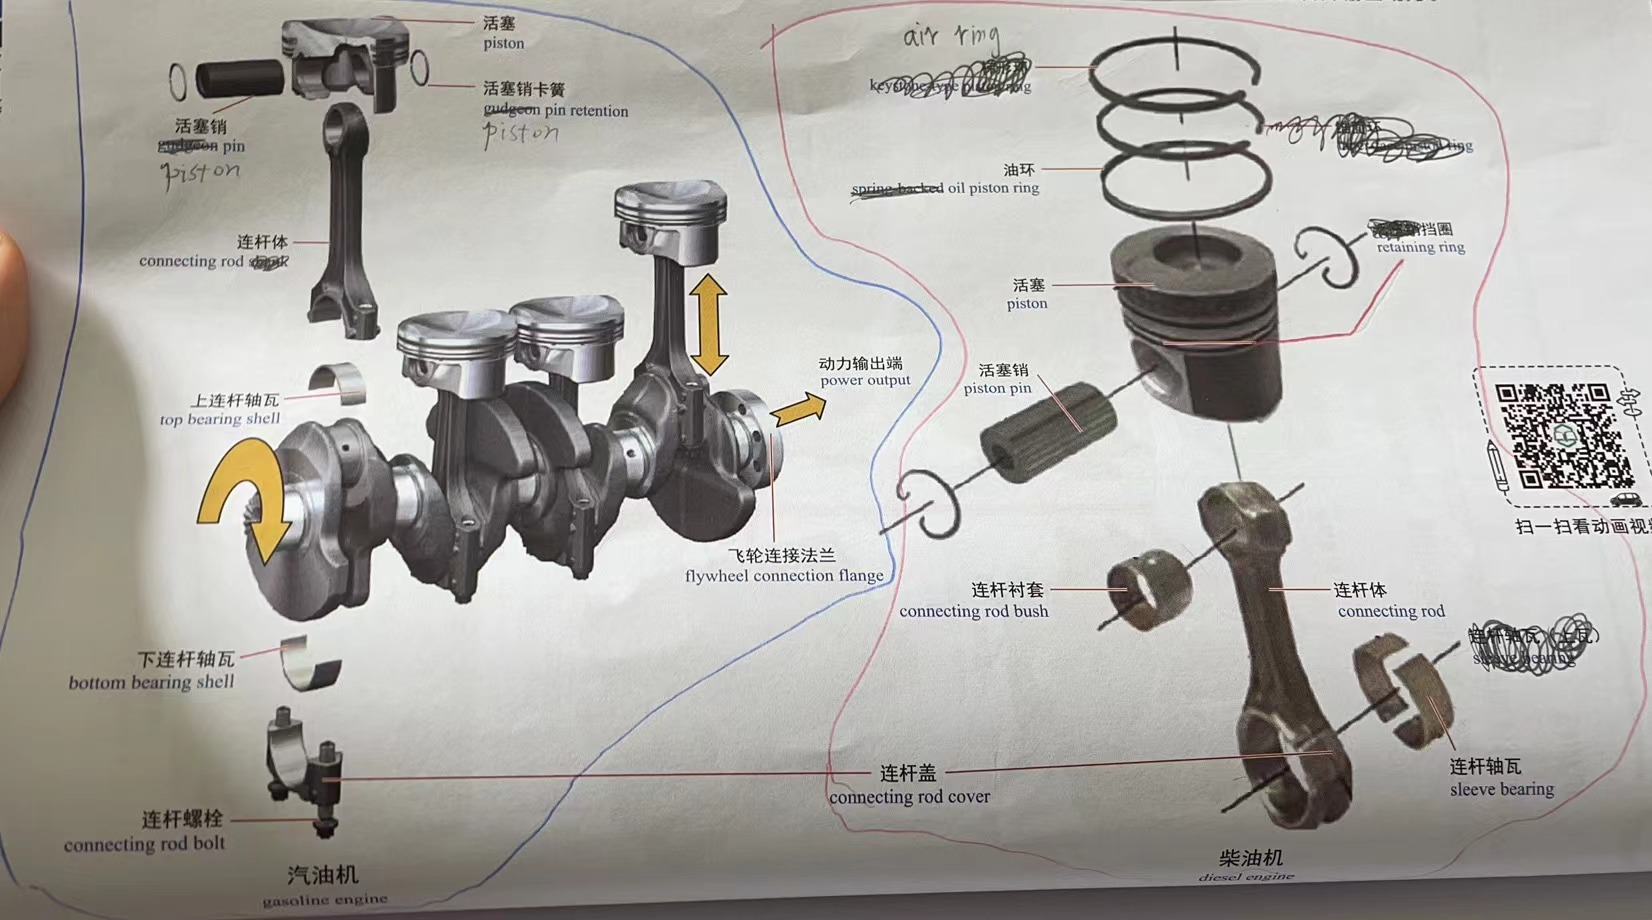
\includegraphics[width=0.9\textwidth]{2-14}
		\end{center}
	\end{block}
\end{frame}
\begin{frame}
	\begin{block}{crankshaft flywheel group}
		function: convert the reciprocating motion of the piston to rotation
		\begin{center}
			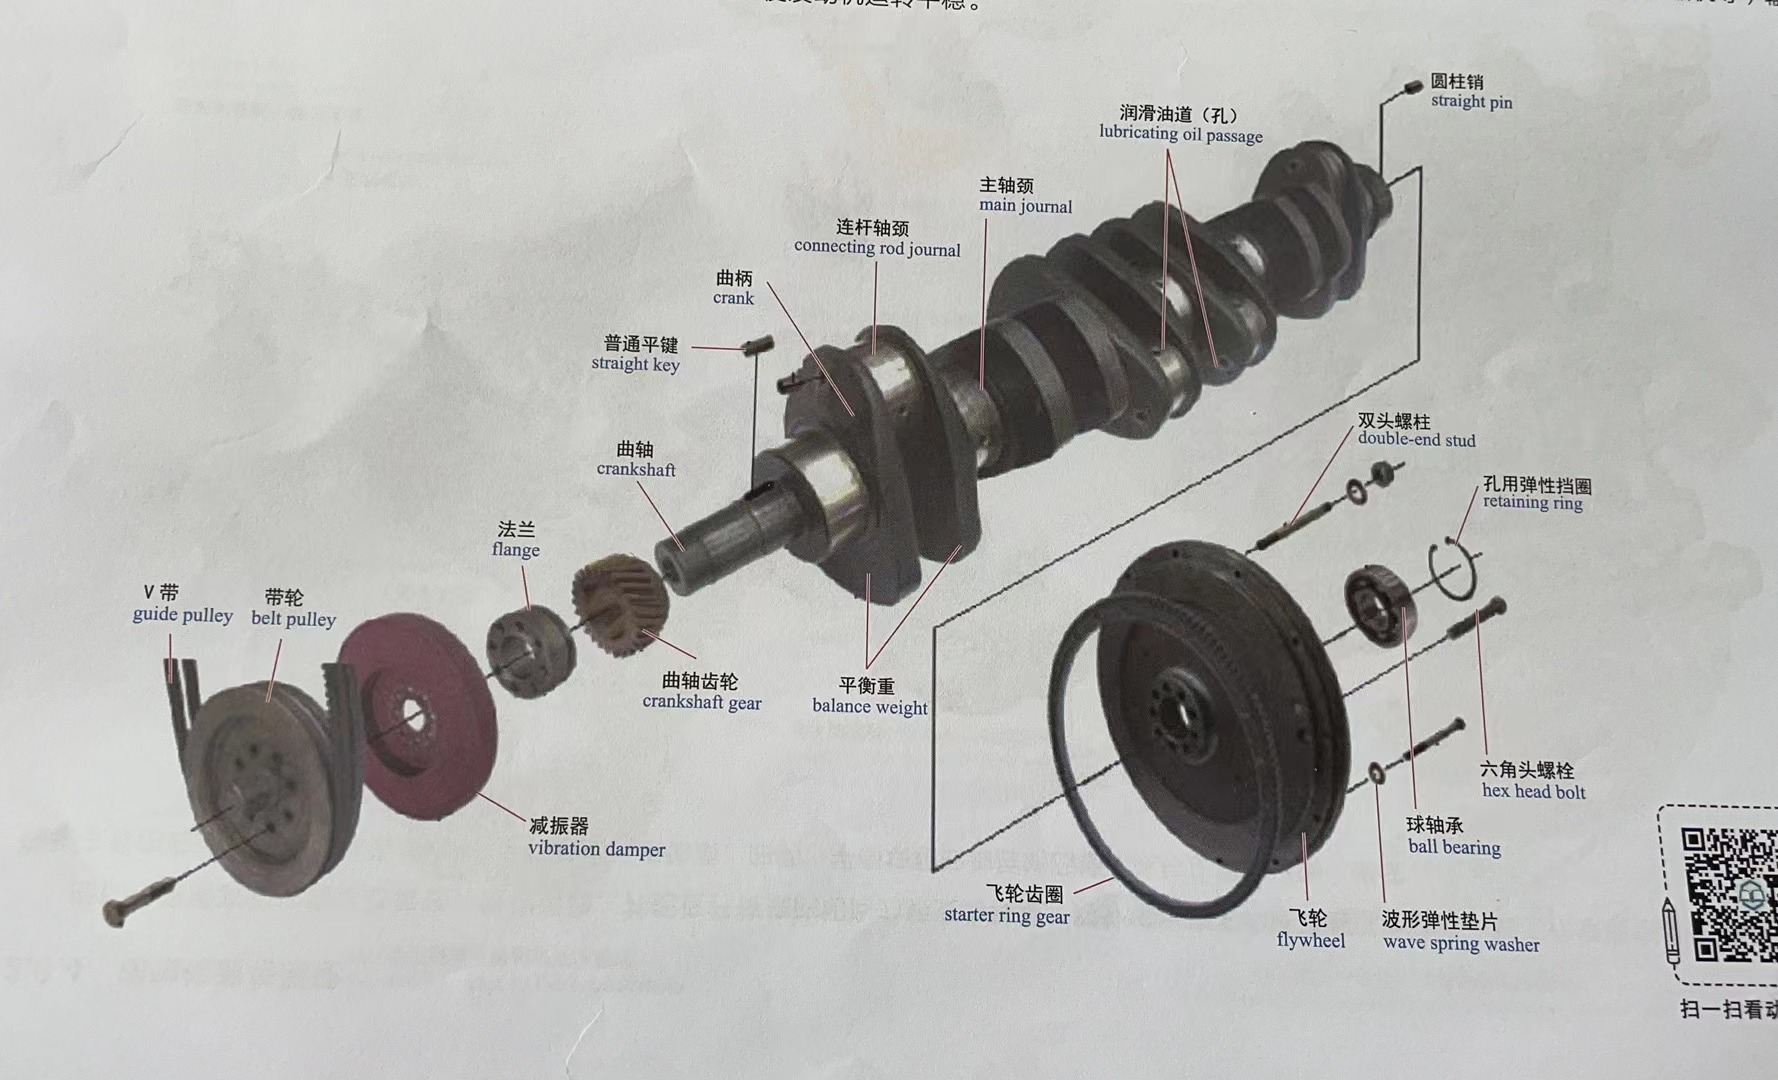
\includegraphics[width=0.8\textwidth]{2-15}
		\end{center}
	\end{block}
\end{frame}
\subsection{配气机构}
\begin{frame}{配气机构}
	\begin{block}{valve group}
		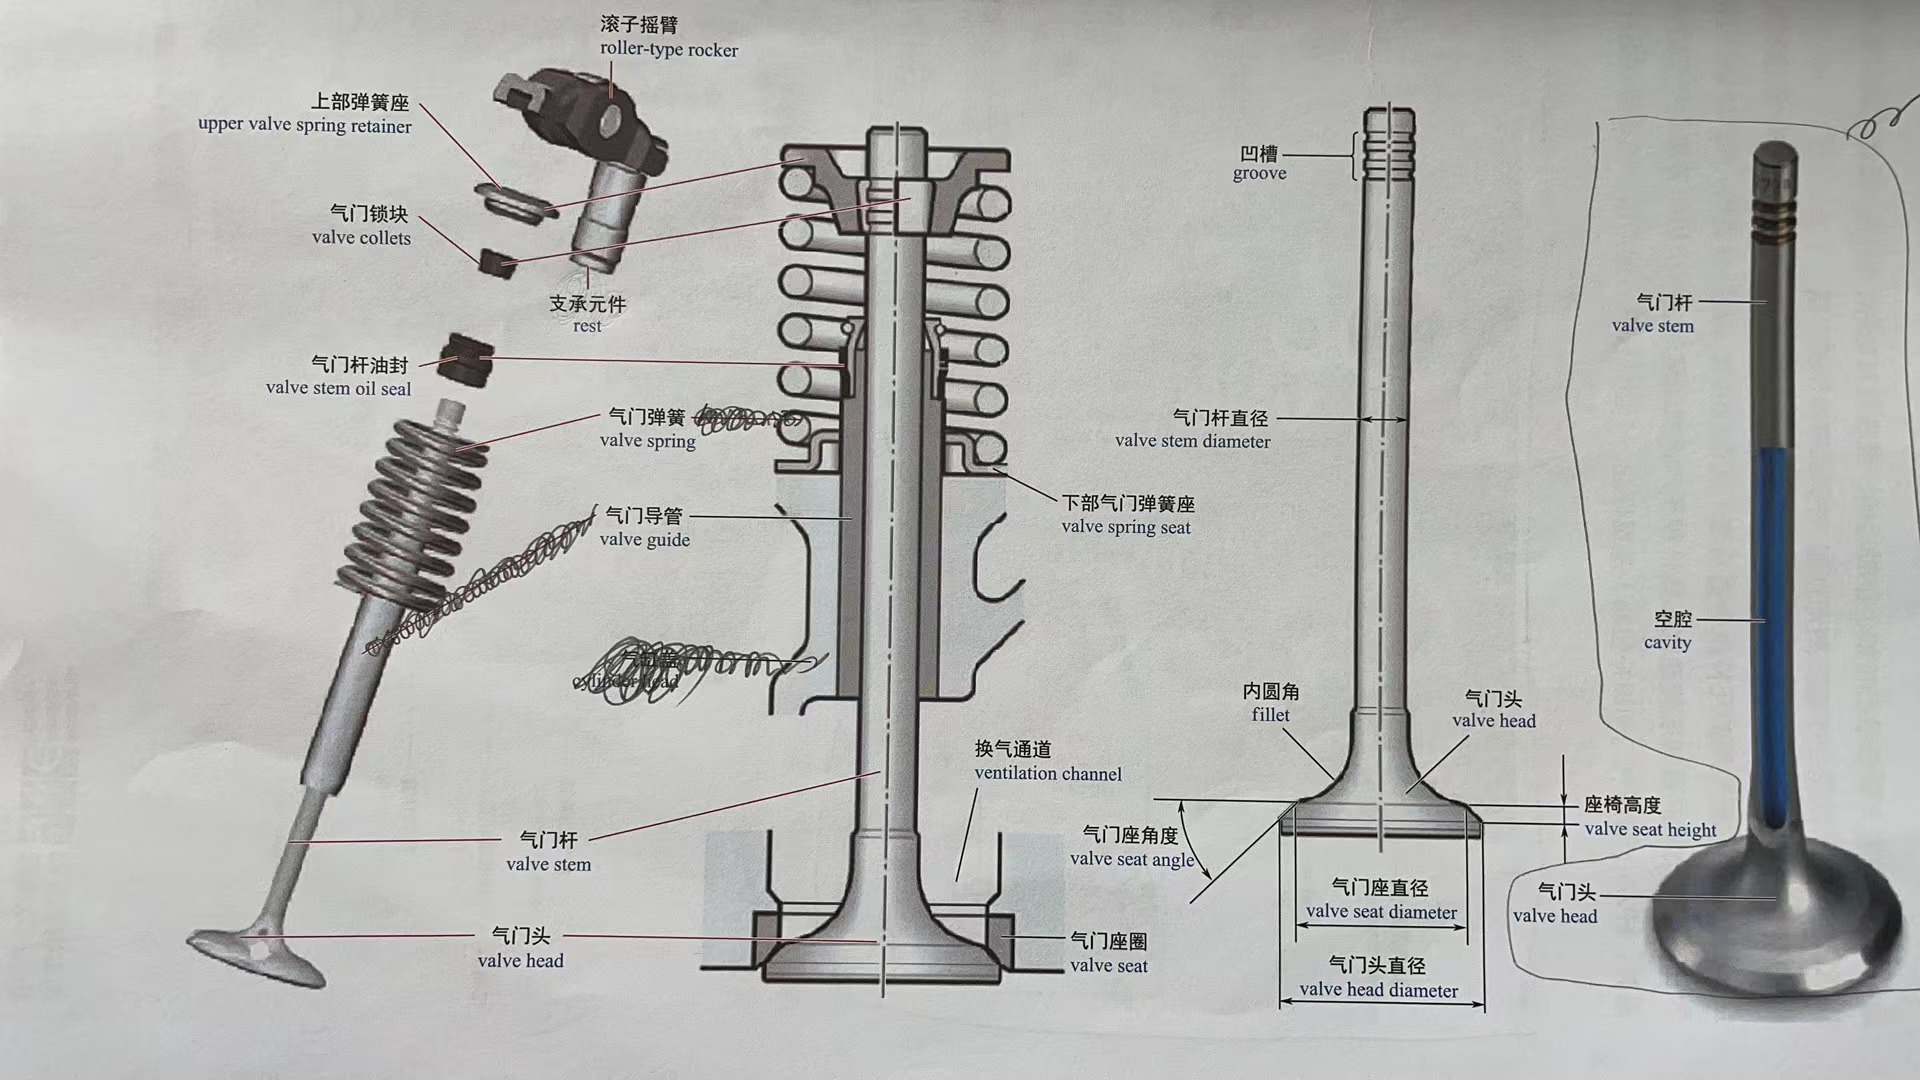
\includegraphics[width=0.9\textwidth]{2-16}
	\end{block}
\end{frame}
\begin{frame}
	\begin{block}{drive group}
		\begin{center}
			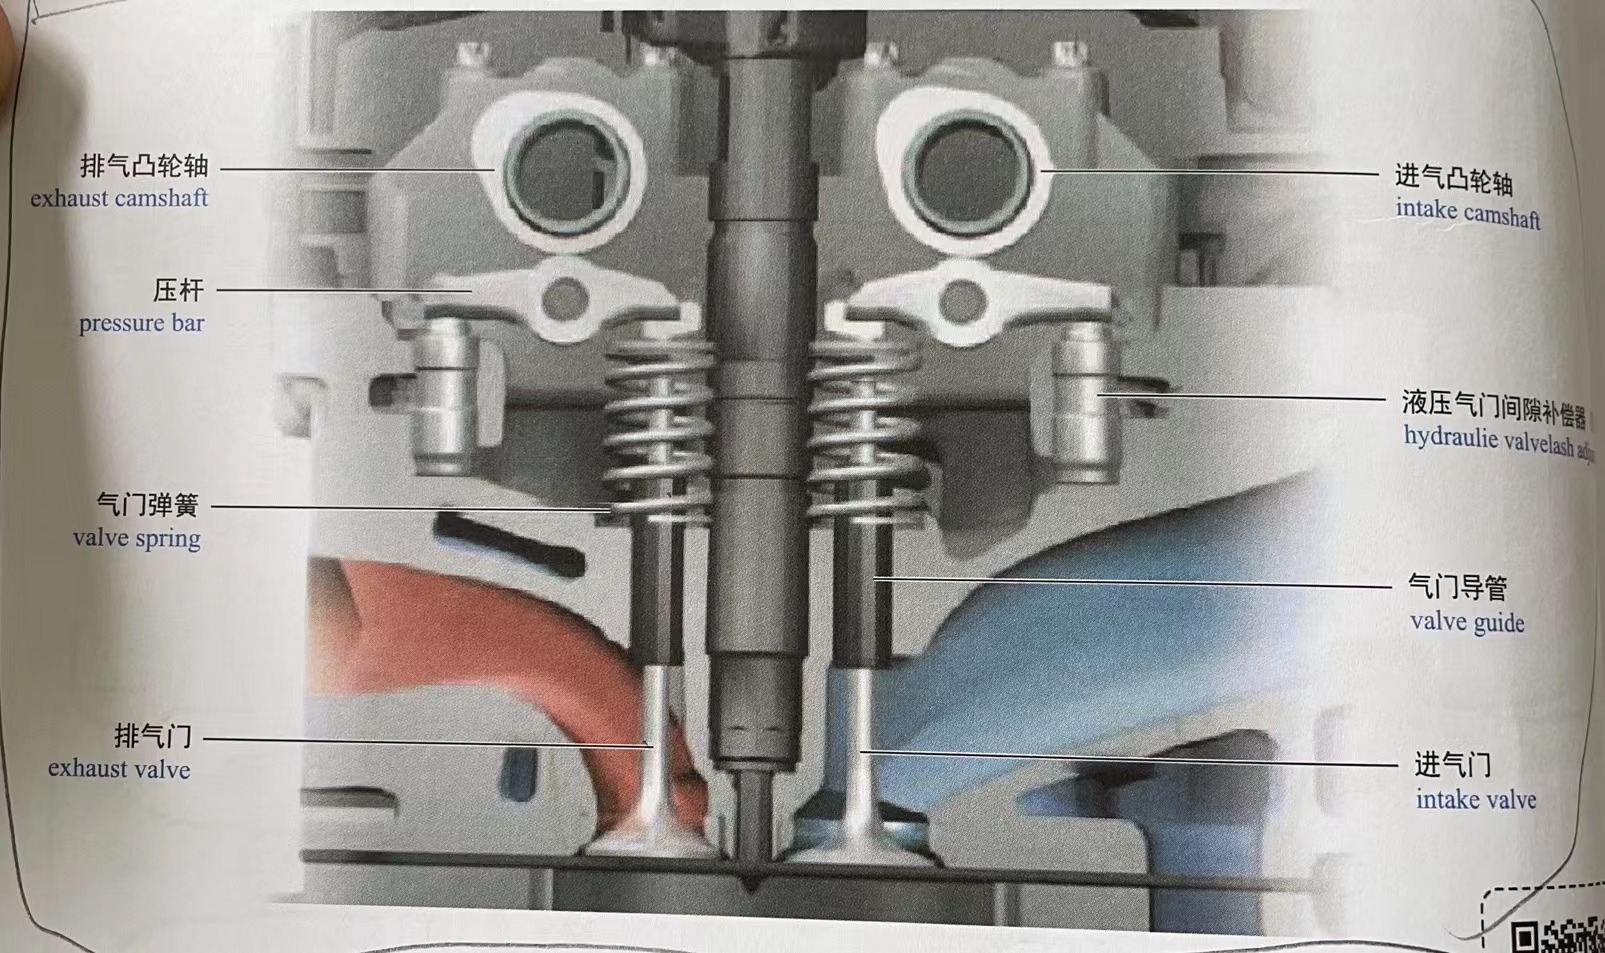
\includegraphics[width=0.9\textwidth]{2-17}
		\end{center}
	\end{block}
\end{frame}
\begin{frame}
	\begin{block}{凸轮轴}
		\begin{figure}[htbp]
			\centering
			\caption{structure of OHC(overhead camshaft)}
			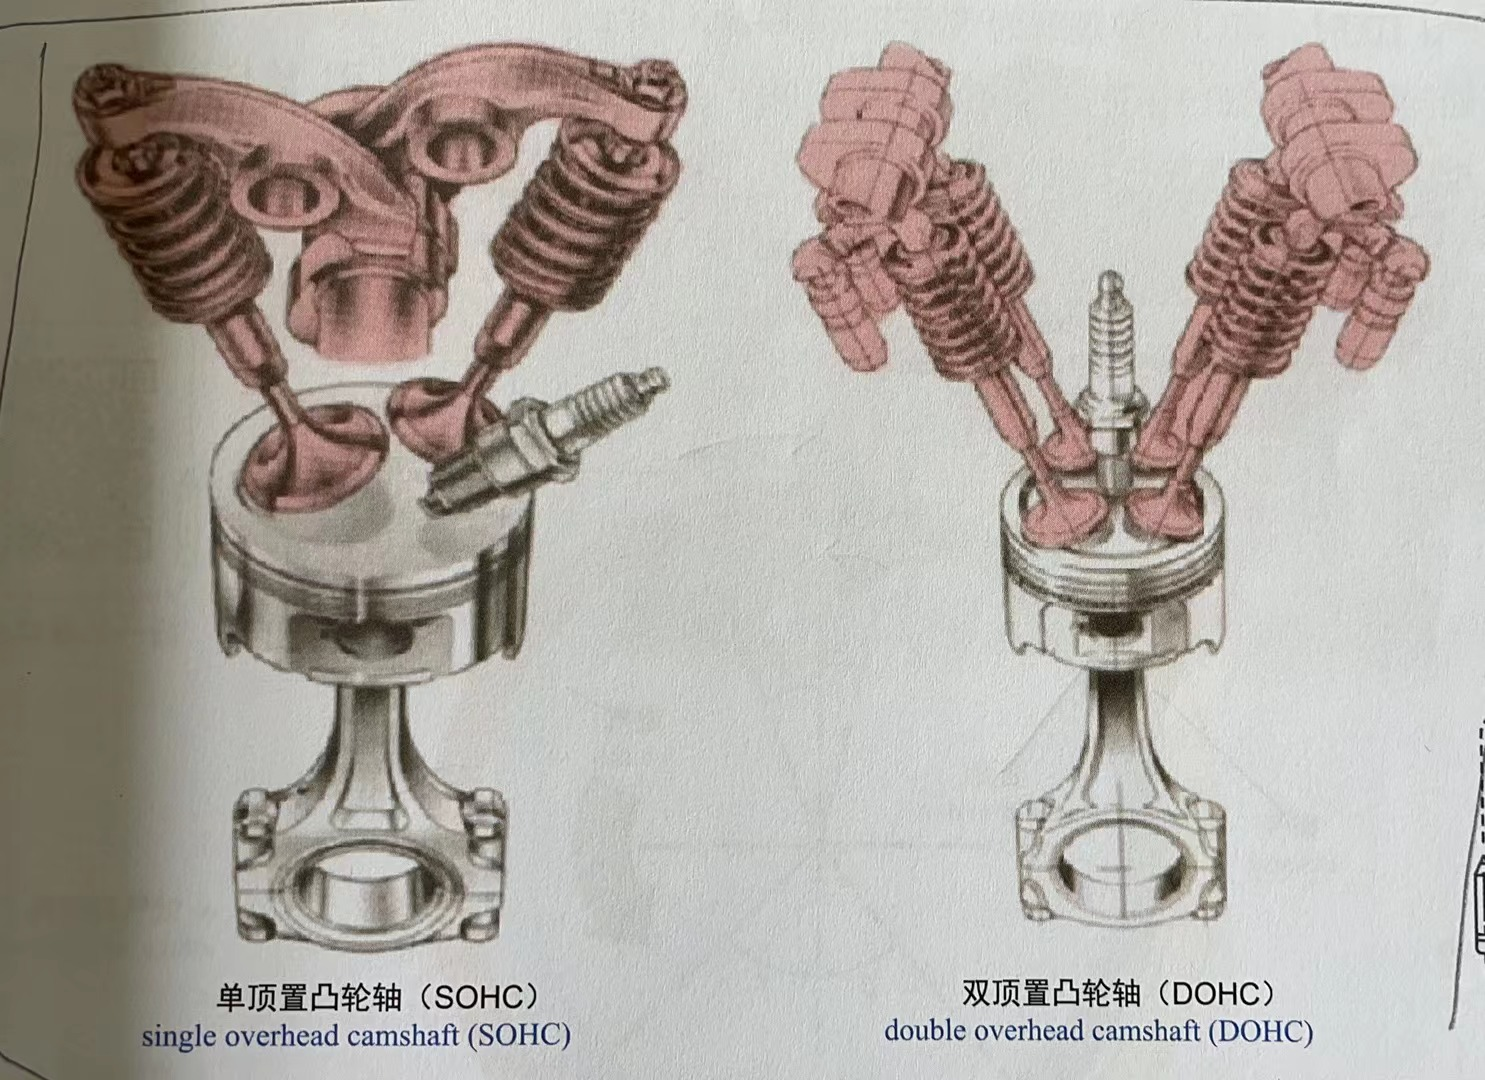
\includegraphics[width=0.9\textwidth]{2-18}
		\end{figure}
	\end{block}
\end{frame}
\begin{frame}
	\begin{block}{气门正时与气门间隙}
		\begin{figure}[htbp]
			\centering
			\subfloat[气门正时]{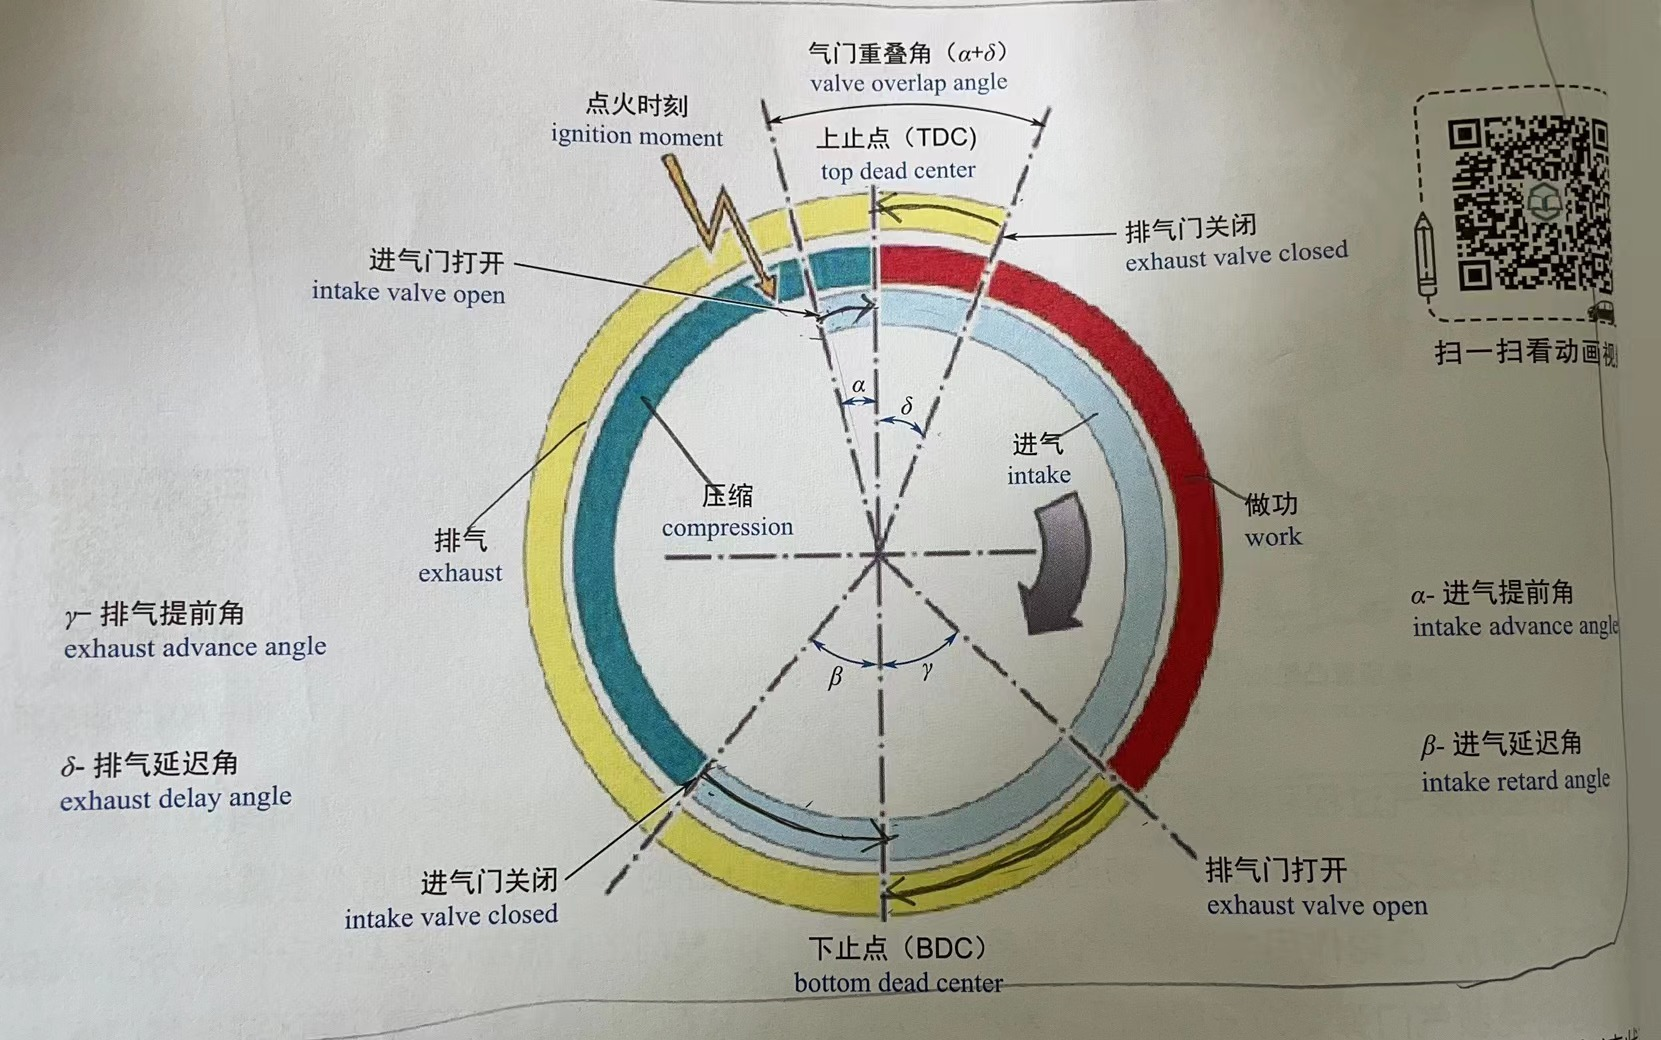
\includegraphics[width=0.5\textwidth]{2-19}}
			\subfloat[气门间隙]{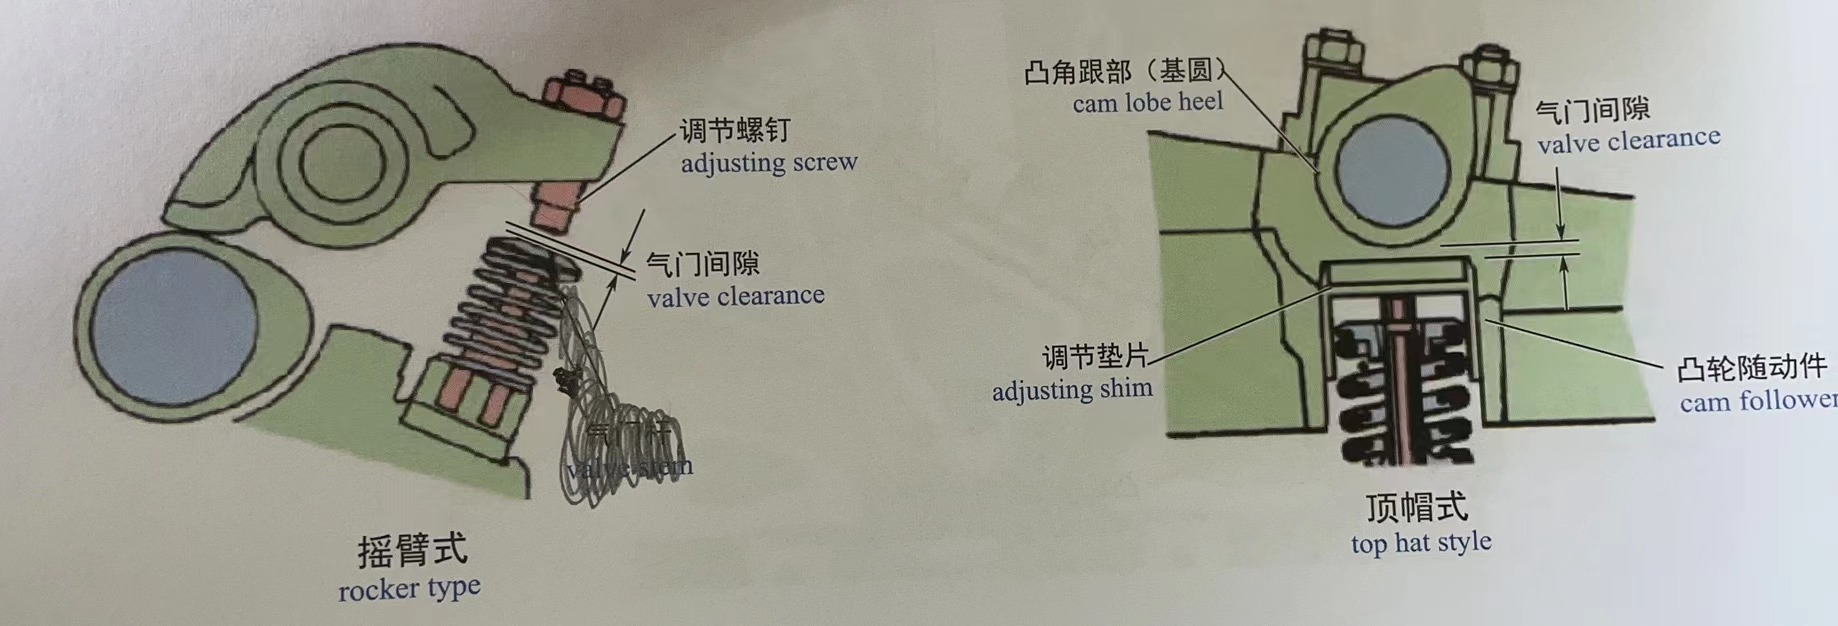
\includegraphics[width=0.5\textwidth]{2-20}}
		\end{figure}
	\end{block}
\end{frame}
\subsection{fuel system}
\begin{frame}{fuel system}
	types: fuel supply system, EFI(electronic fuek ubhecruib电控燃油喷射),GDI(gasoline direct injection缸内直喷),GRDI(common rail direct inject 燃油高压共轭系统), UIS(unit injector system柴油泵喷嘴系统)、UPS(unit pump system柴油单体泵系统)
\end{frame}
\begin{frame}
	\begin{block}{fuel supply system}
		\begin{center}
			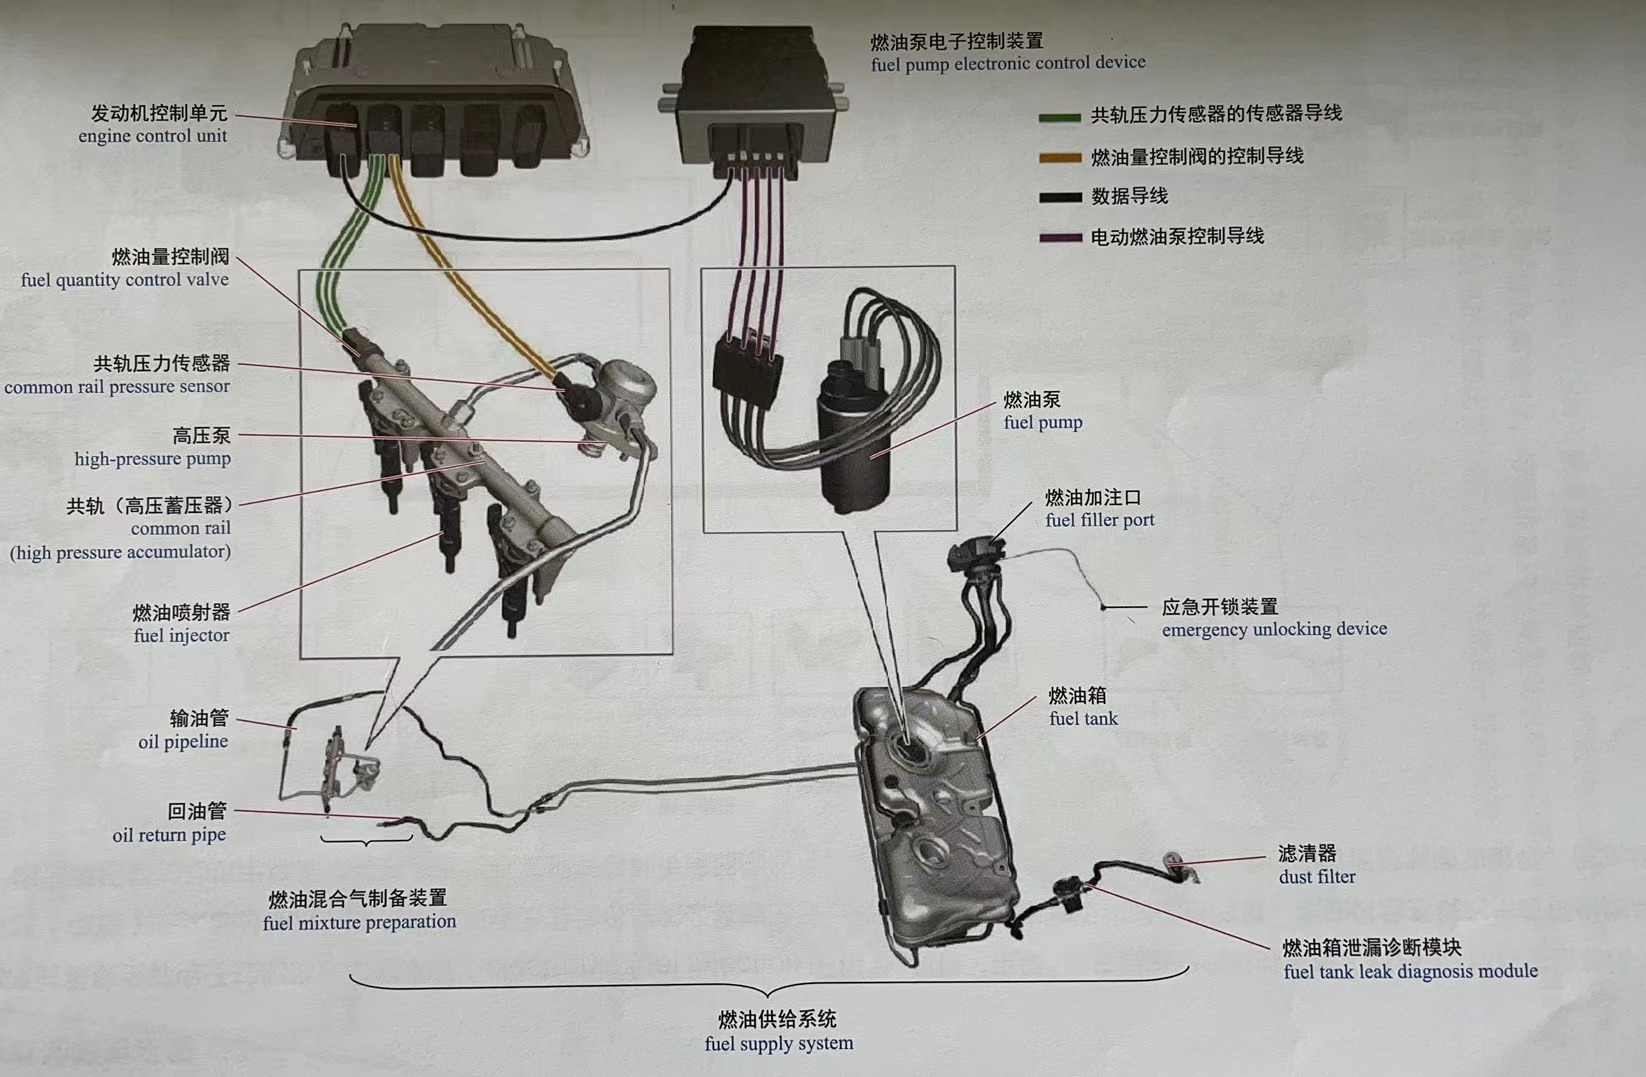
\includegraphics[width=0.9\textwidth]{2-21}
		\end{center}
	\end{block}
\end{frame}
\begin{frame}
	\begin{block}{EFI电控燃油喷射}
		It's composed of air supply system, fuel supply system, control sys
		\begin{center}
			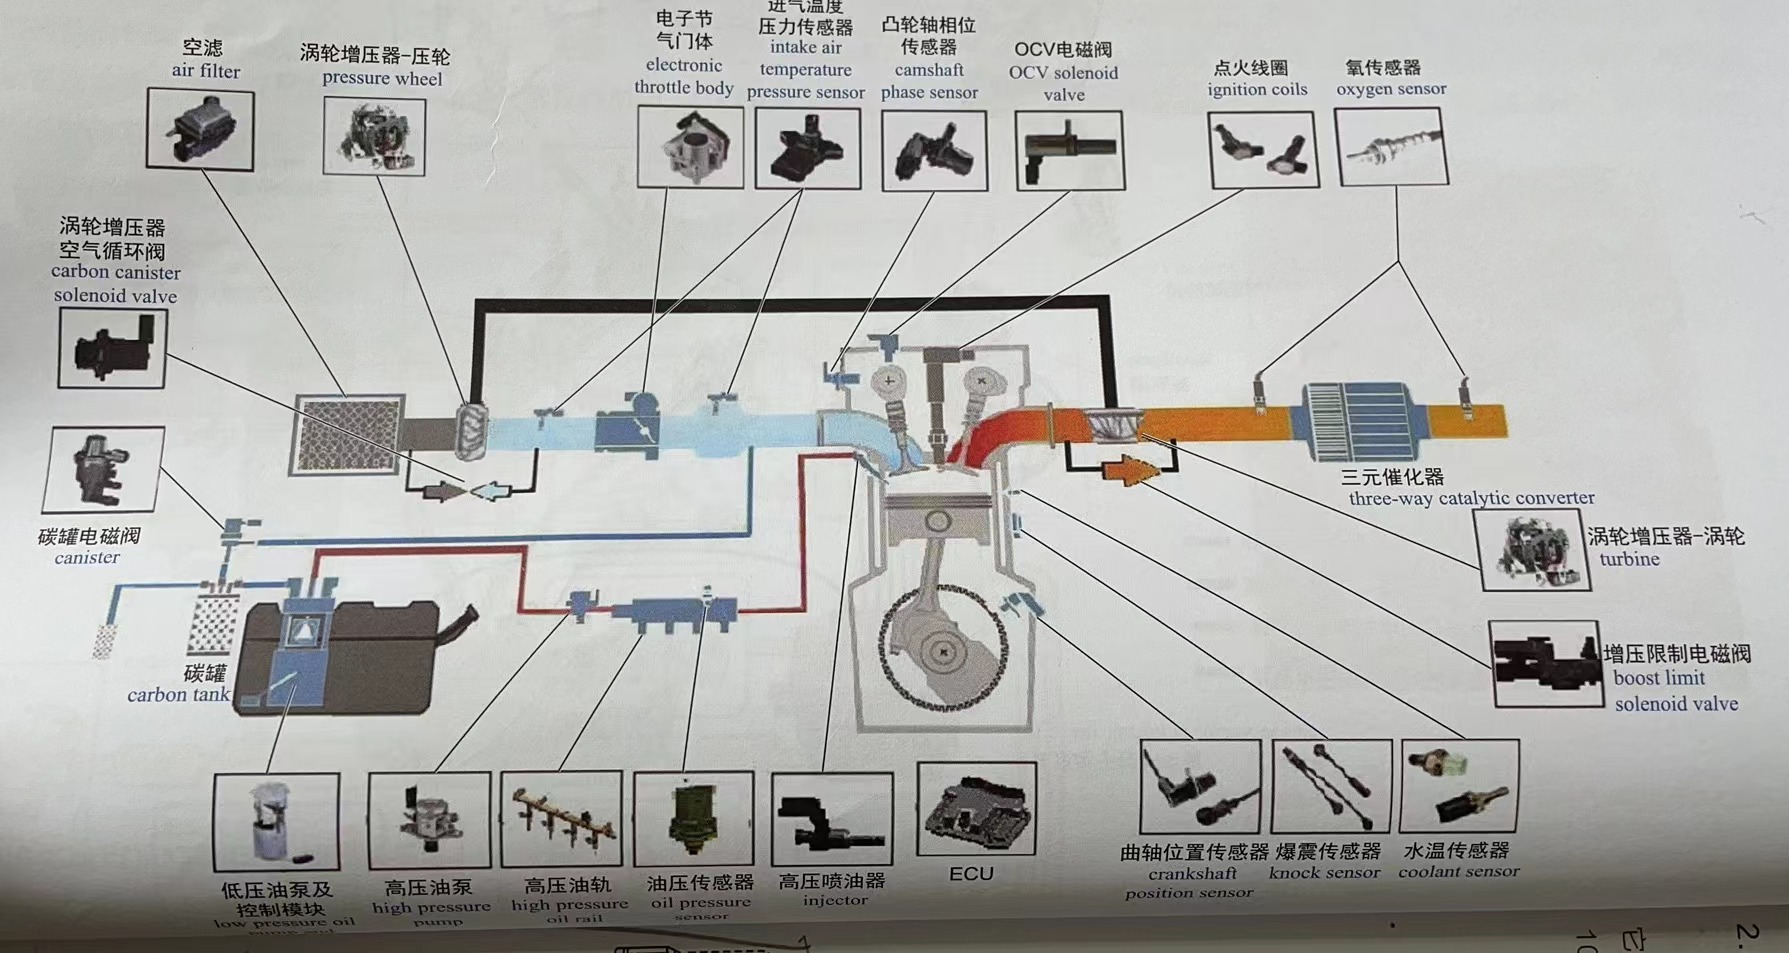
\includegraphics[width=0.9\textwidth]{2-22}
		\end{center}
	\end{block}
\end{frame}
\begin{frame}
	\begin{block}{GDI(gasoline direct injection缸内直喷)}
		\begin{center}
			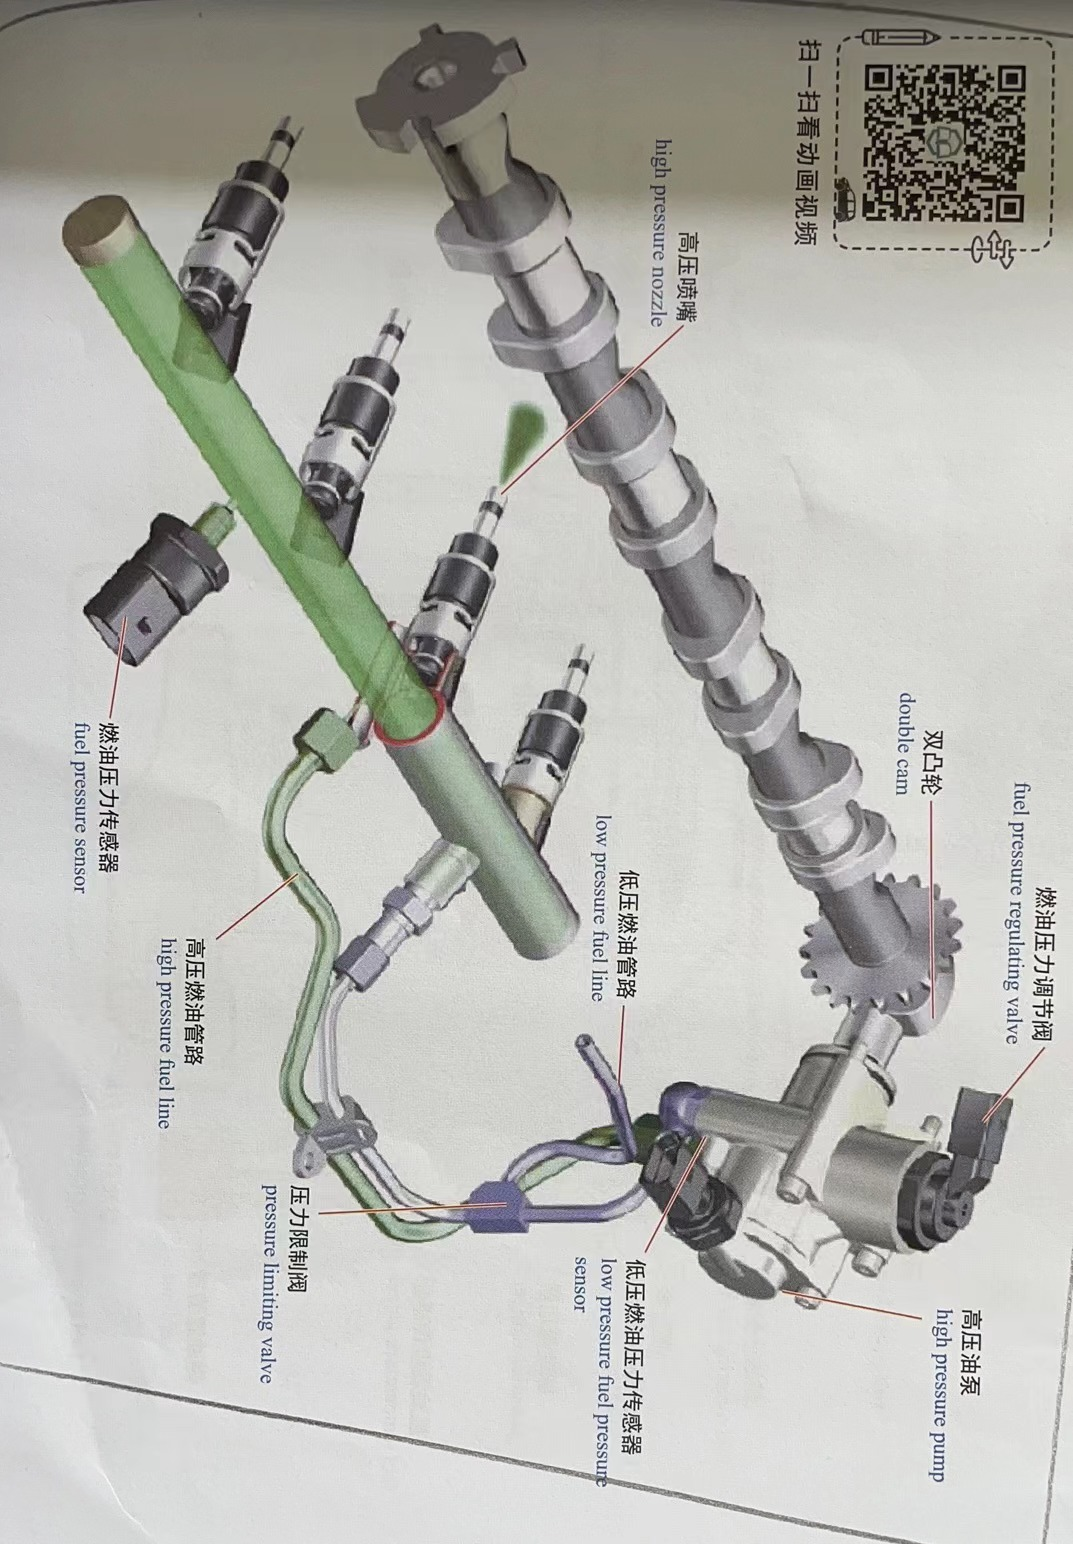
\includegraphics[angle=90,width=0.5\textwidth]{2-23}
		\end{center}
	\end{block}
\end{frame}
\begin{frame}
	\begin{block}{GRDI(common rail direct inject 燃油高压共轭系统)}
		\begin{center}
			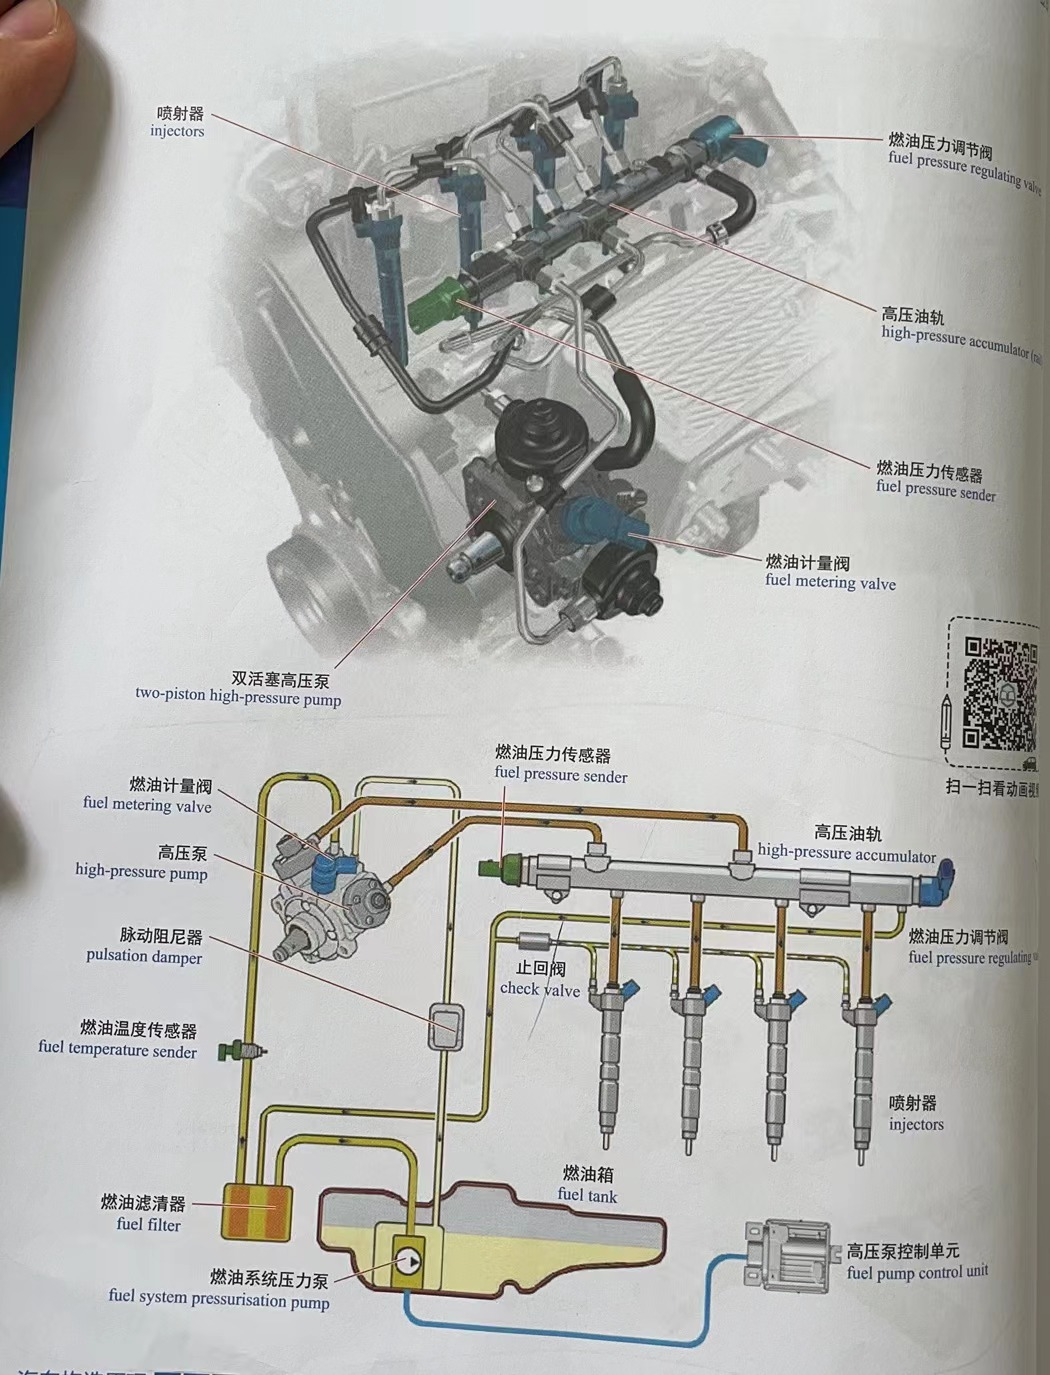
\includegraphics[width=0.5\textwidth]{2-24}
		\end{center}
	\end{block}
\end{frame}
\begin{frame}
	\begin{block}{UIS(unit injector system柴油泵喷嘴系统)}
		\begin{center}
			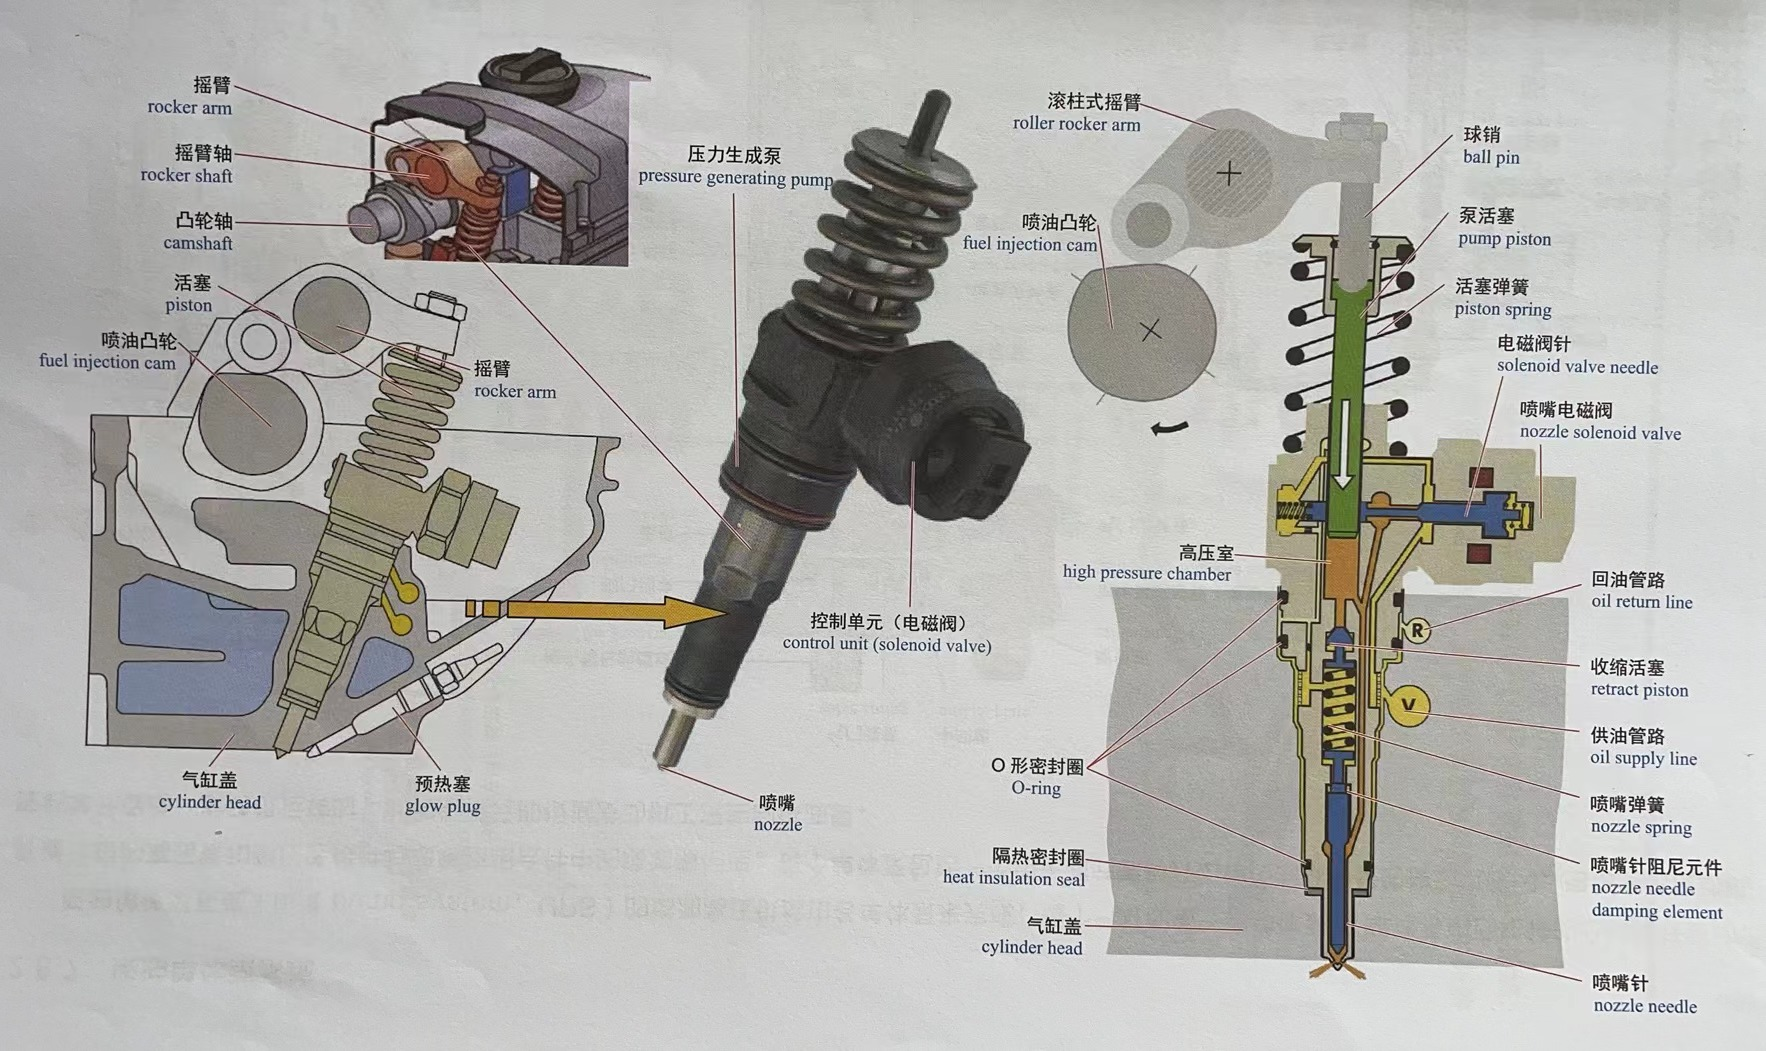
\includegraphics[width=0.9\textwidth]{2-25}
		\end{center}
	\end{block}
\end{frame}
\begin{frame}
	\begin{block}{UPS(unit pump system柴油单体泵系统)}
		\begin{center}
			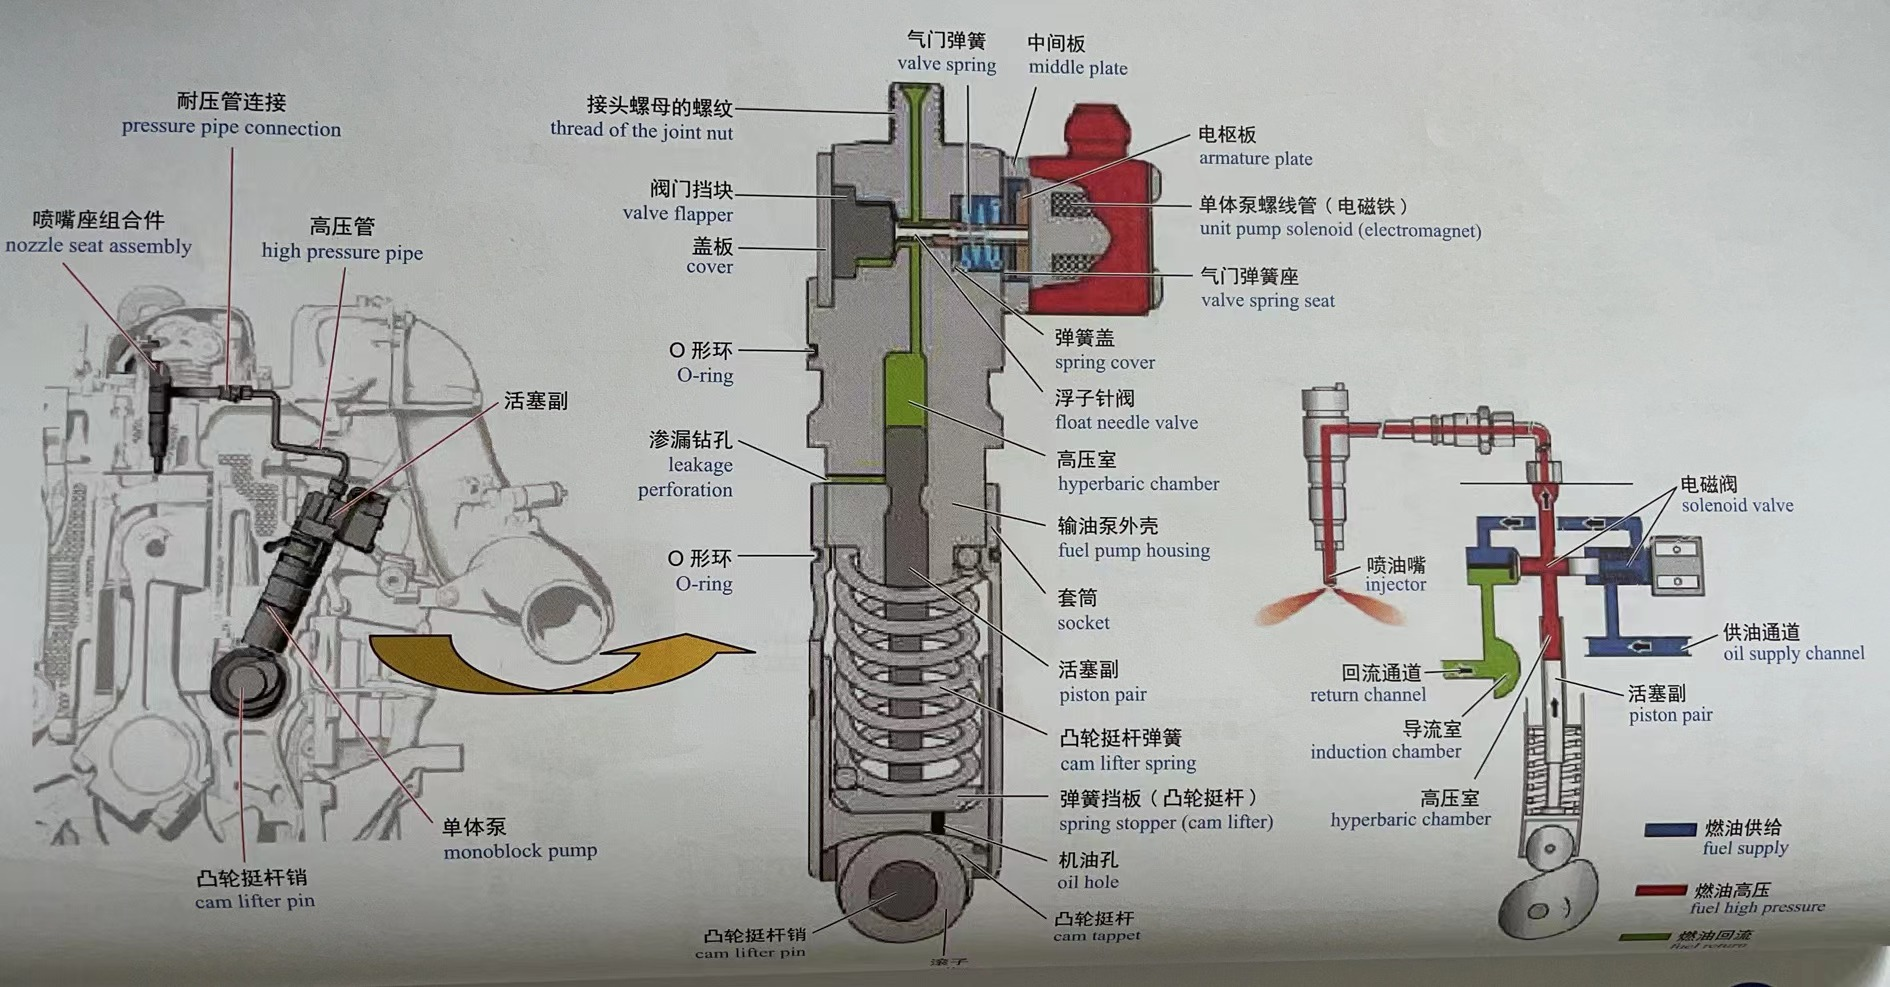
\includegraphics[width=0.9\textwidth]{2-26}
		\end{center}
	\end{block}
\end{frame}
\subsection{intake and exhaust system}
\begin{frame}{intake and exhaust system}
	\begin{block}{intake system}
		\begin{center}
			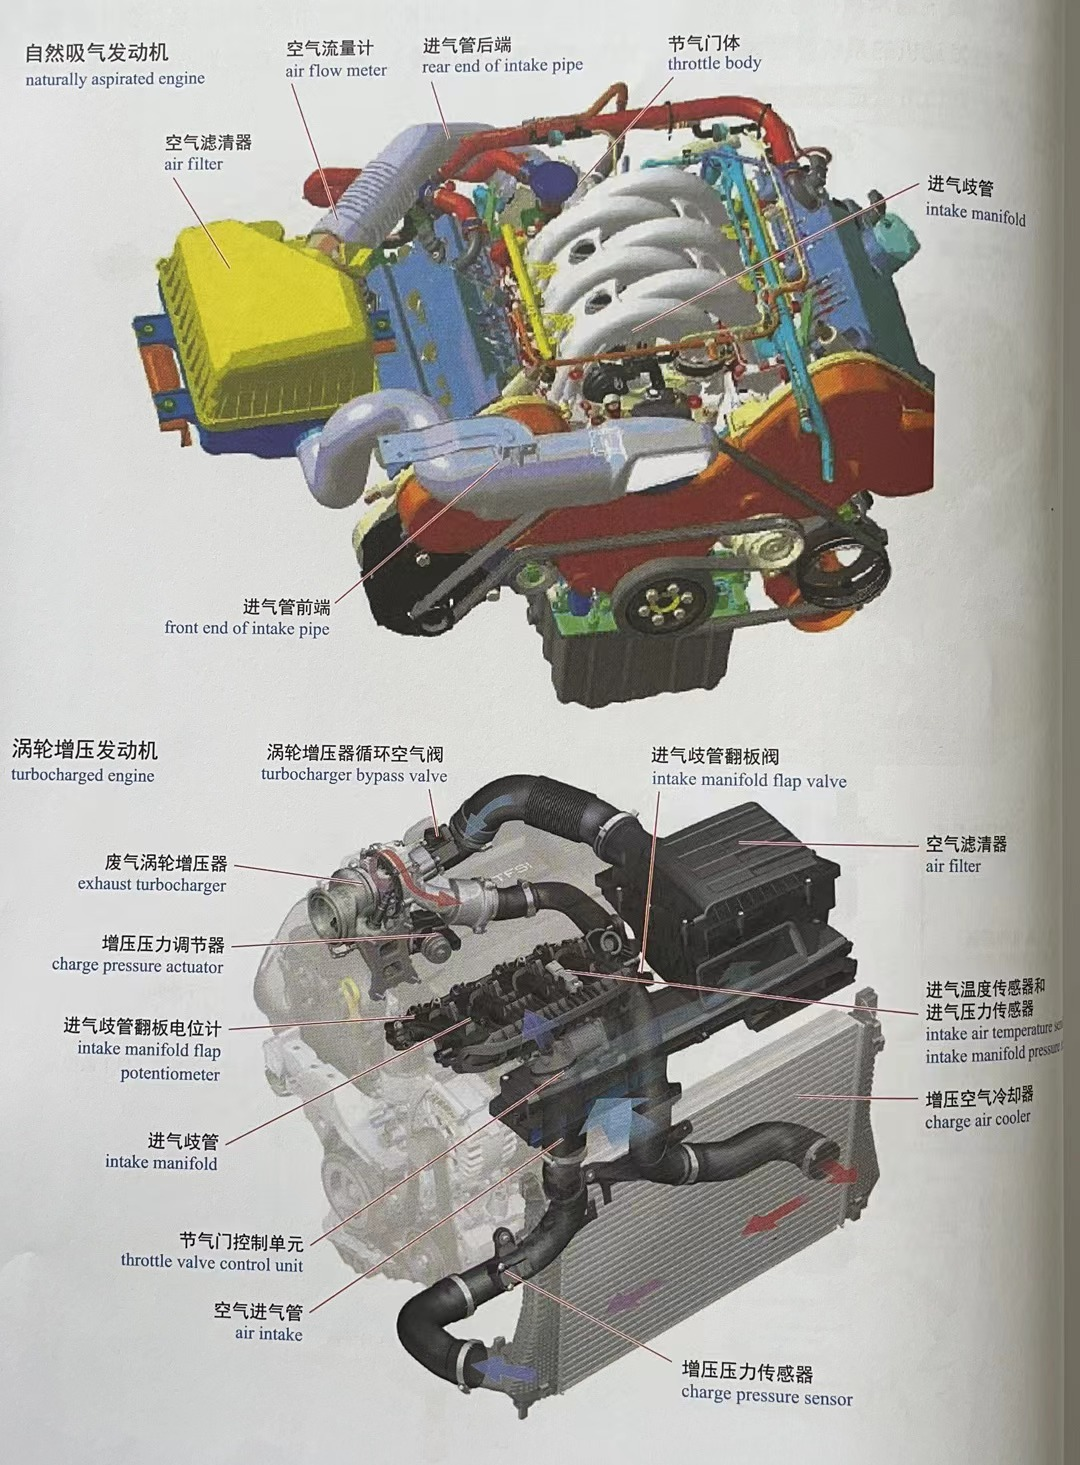
\includegraphics[width=0.4\textwidth]{2-27}
		\end{center}
	\end{block}
\end{frame}
\begin{frame}
	\begin{block}{exhaust system}
		\begin{center}
			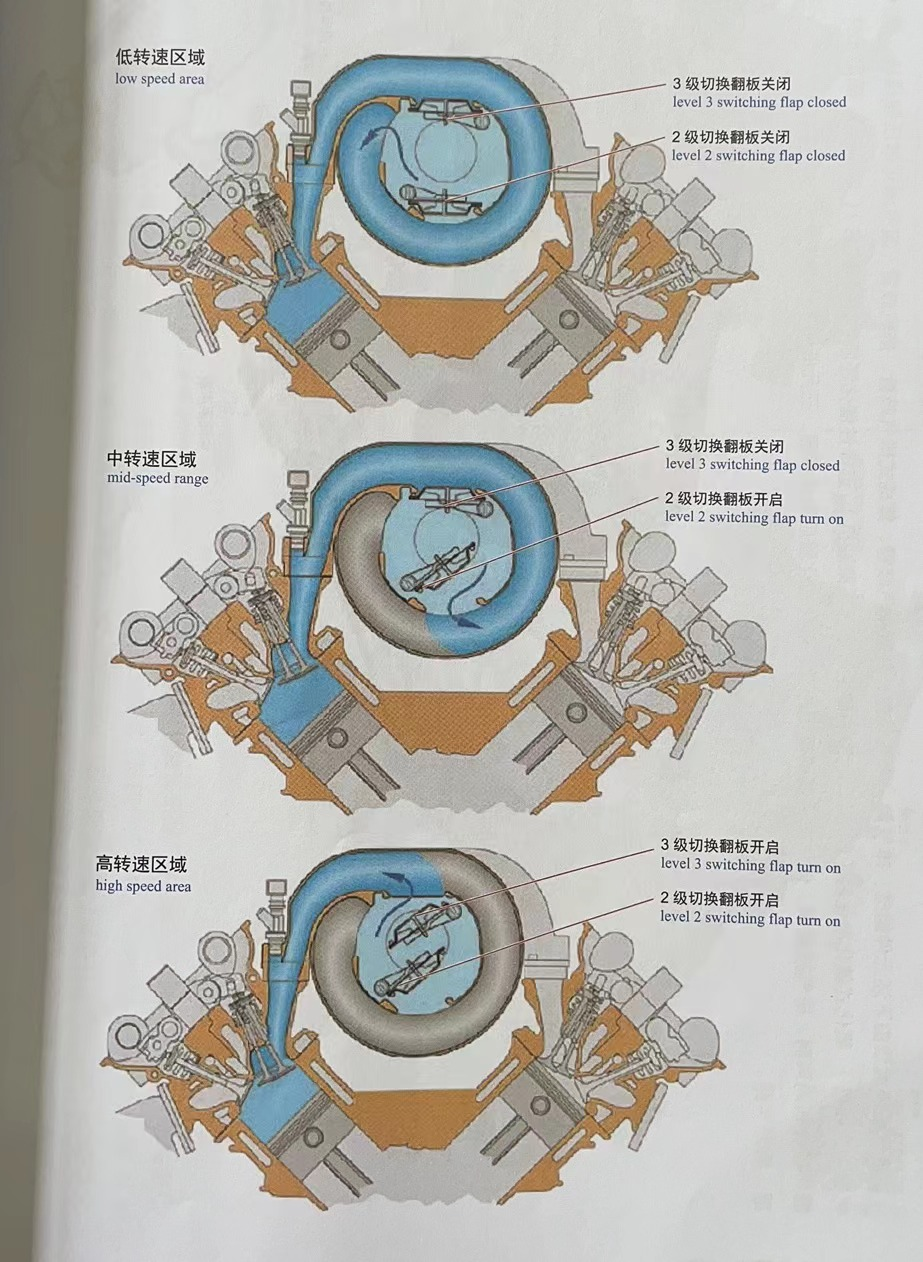
\includegraphics[width=0.4\textwidth]{2-28}
		\end{center}
	\end{block}
\end{frame}
\begin{frame}
	\begin{block}{涡轮增压器}
		\begin{center}
			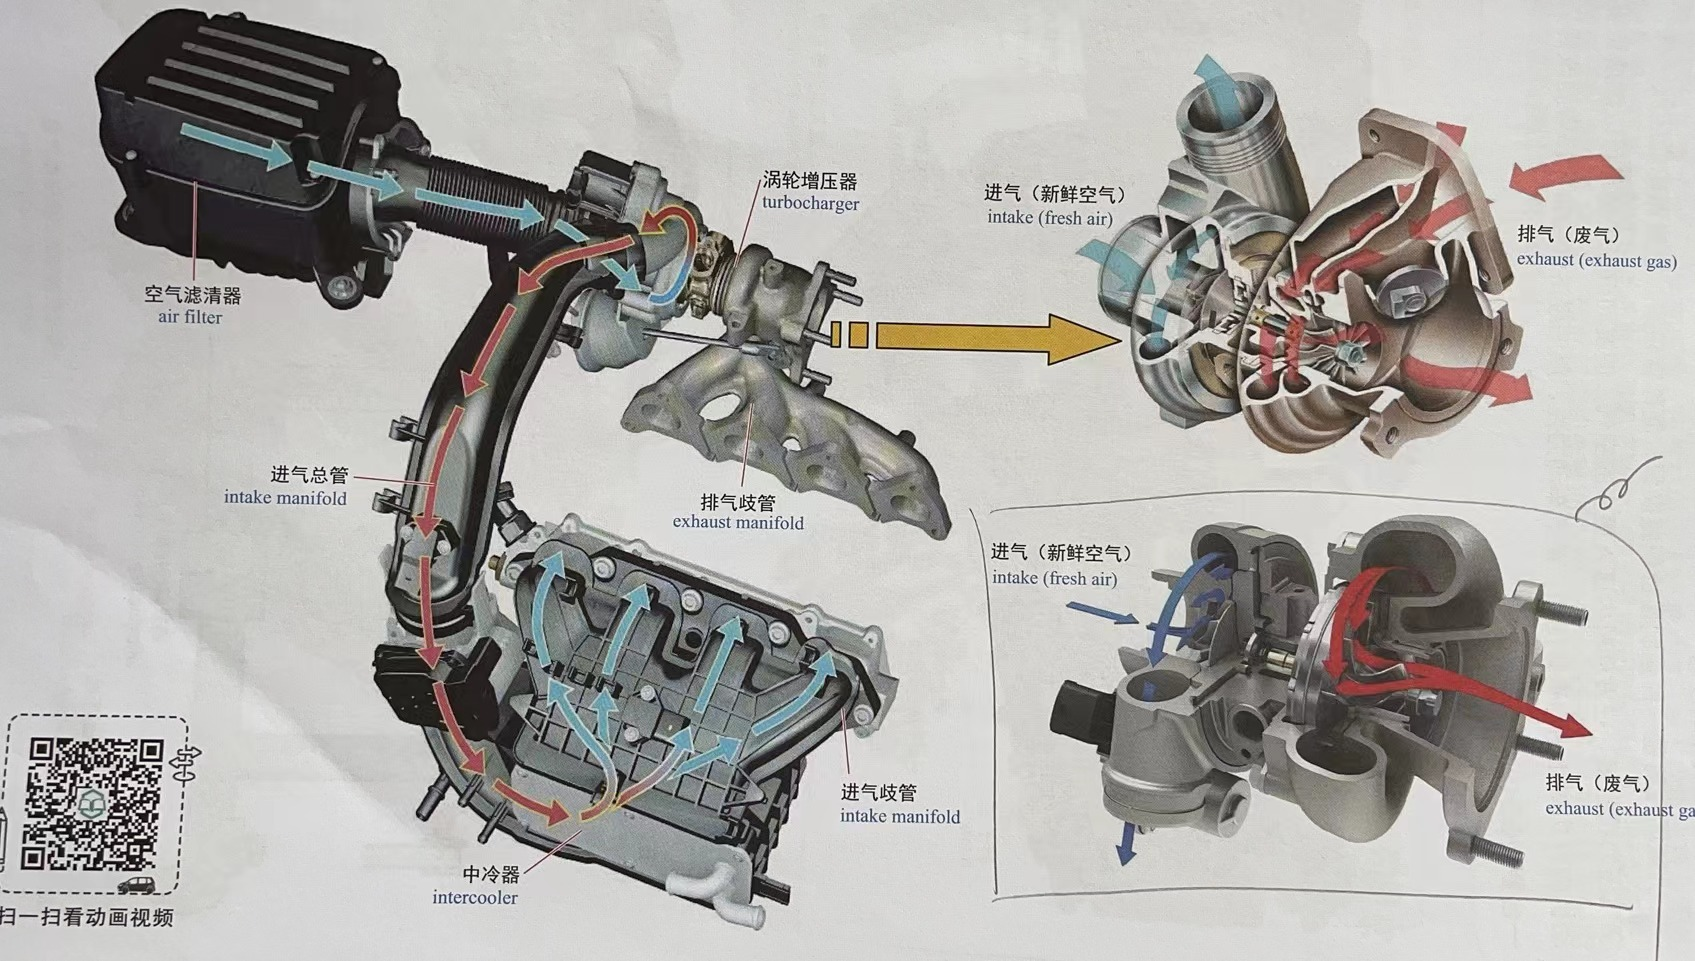
\includegraphics[width=0.8\textwidth]{2-29}
		\end{center}
	\end{block}
\end{frame}
\begin{frame}
	\begin{block}{机械增压器}
		\begin{figure}[htbp]
			\centering
			\subfloat[普通]{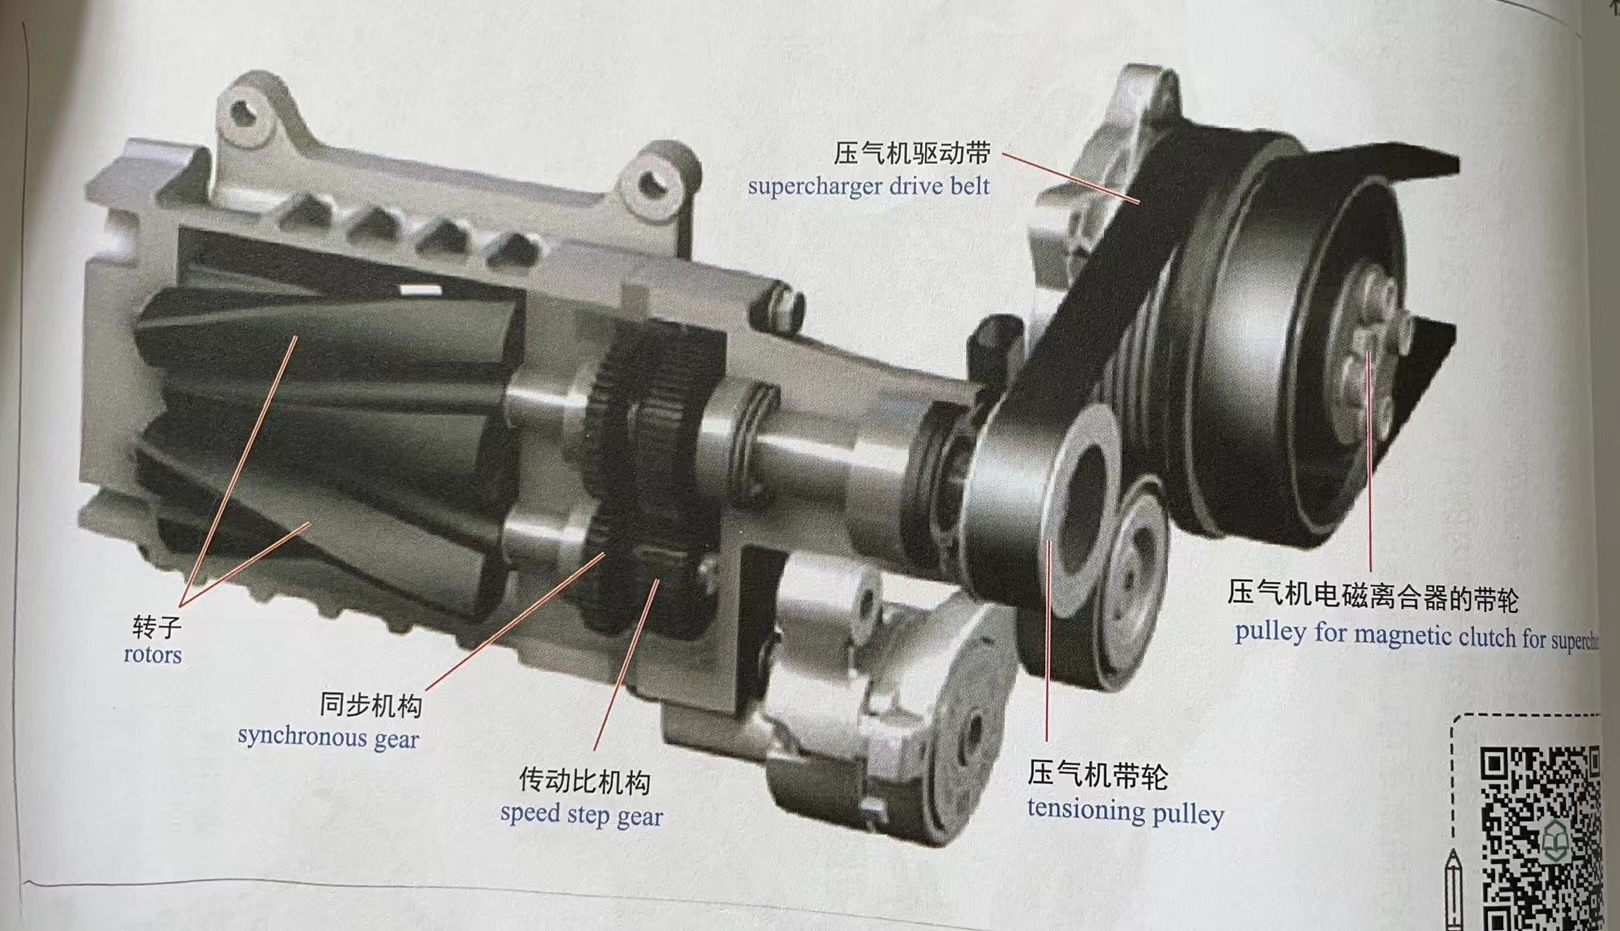
\includegraphics[width=0.5\textwidth]{2-30}}
			
			\subfloat[罗兹式增压器]{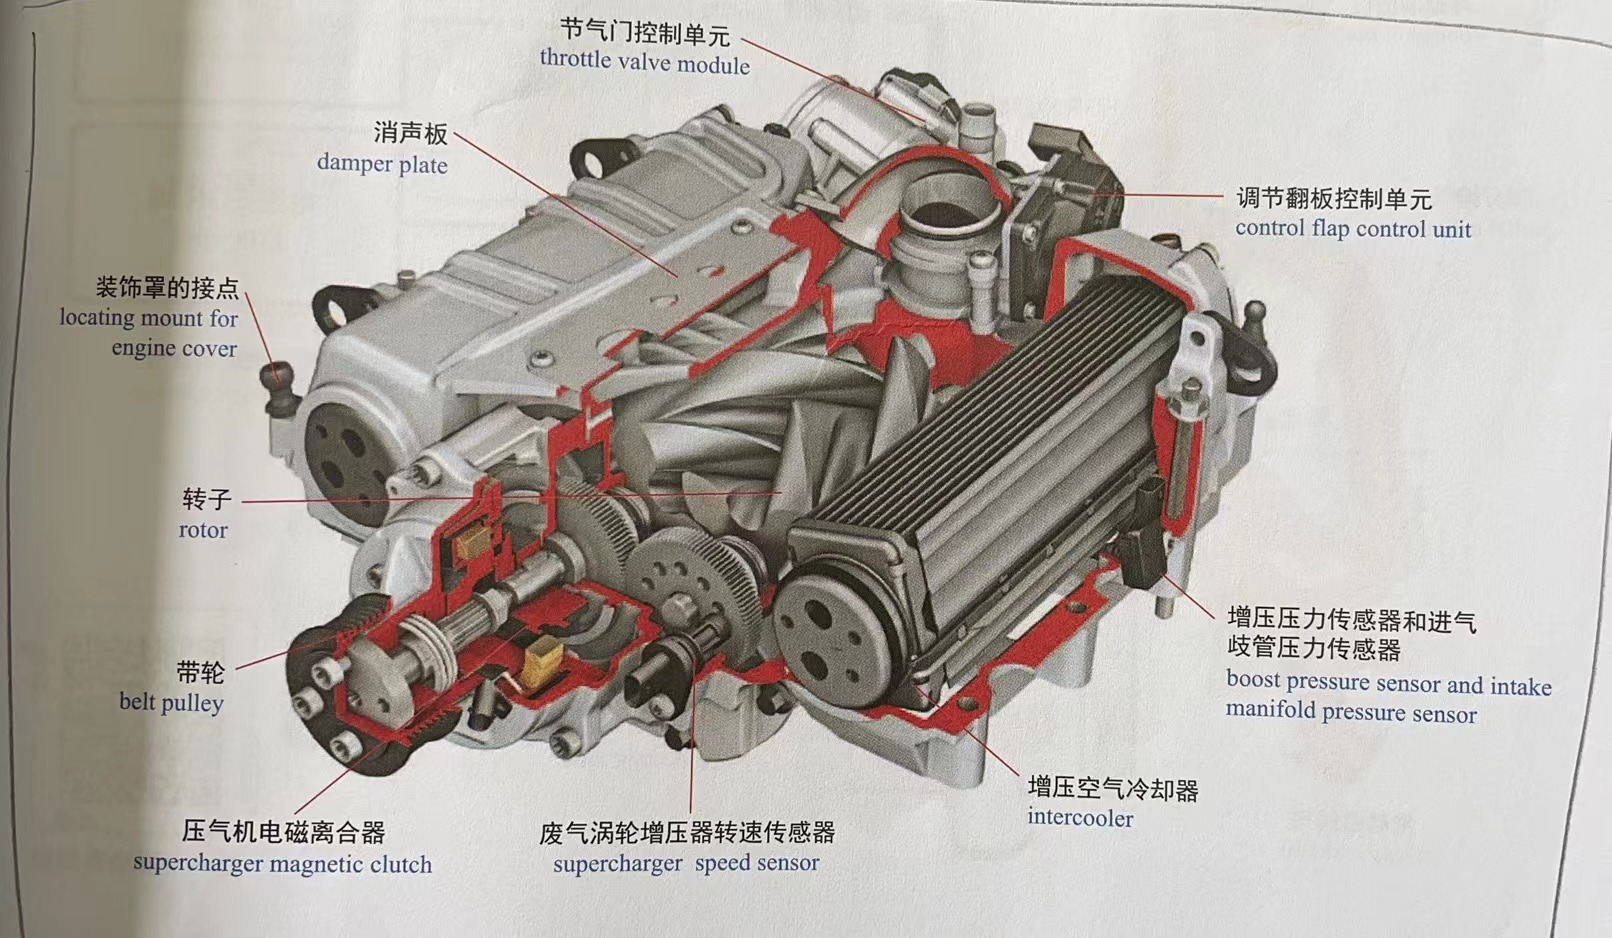
\includegraphics[width=0.5\textwidth]{2-31}}
		\end{figure}
	\end{block}
\end{frame}
\begin{frame}
	\begin{block}{EGR废气再循环系统}
		是排气系统的一部分
		\begin{center}
			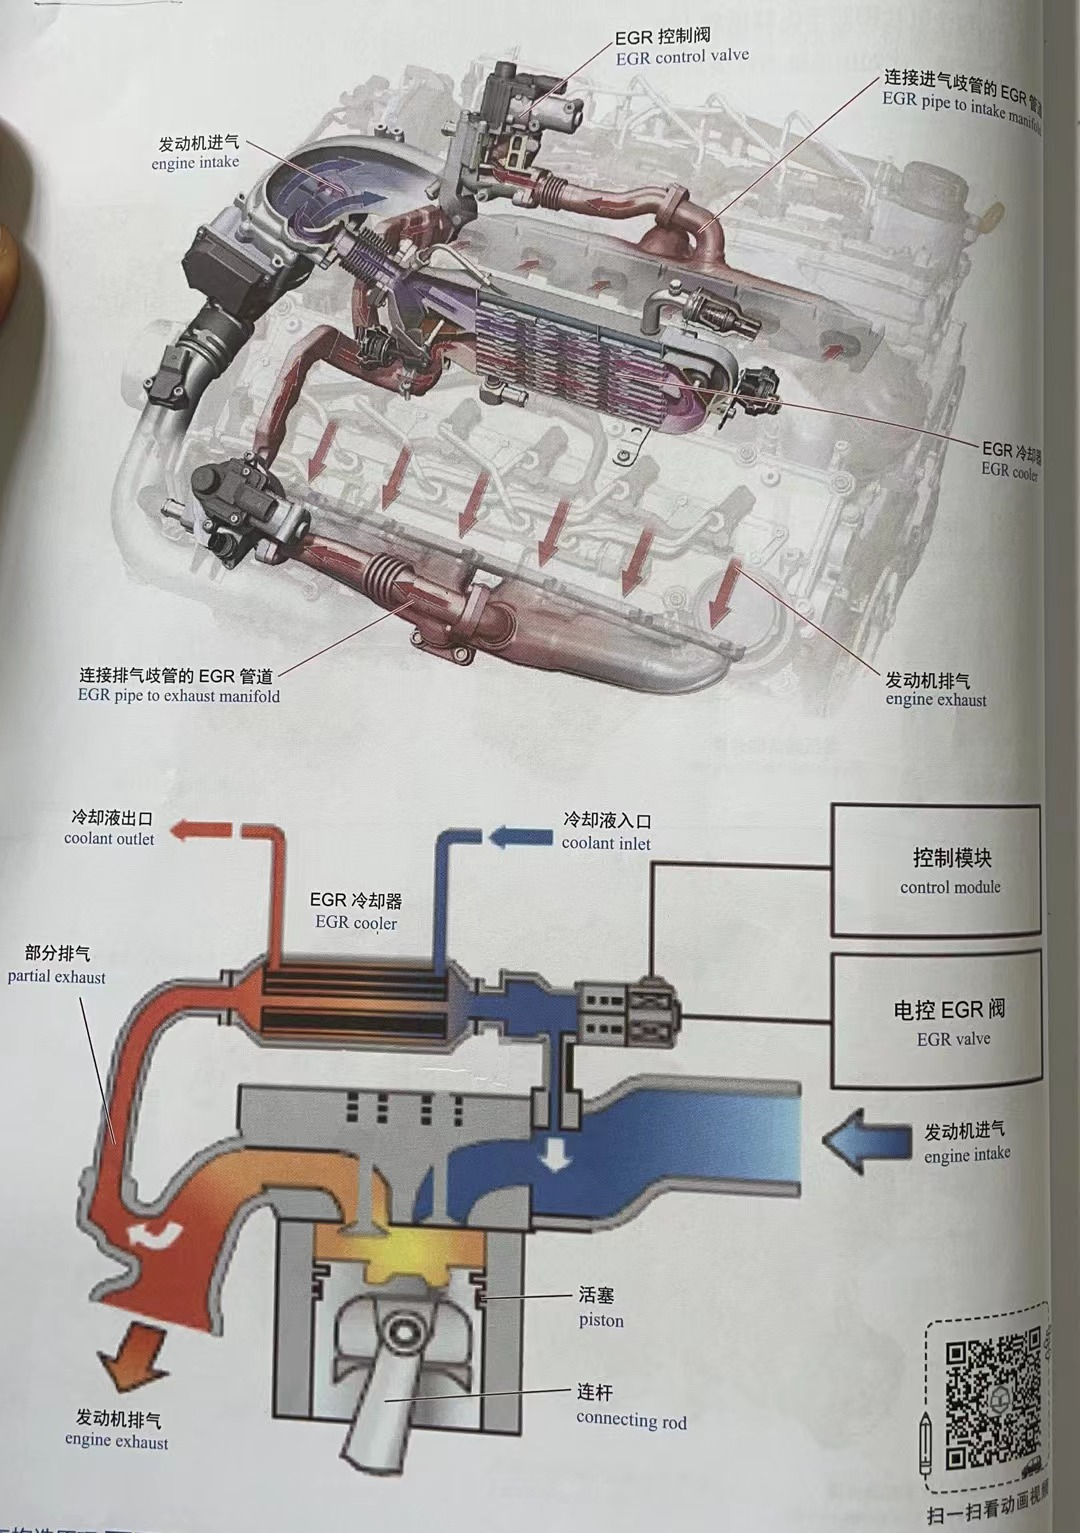
\includegraphics[width=0.44\textwidth]{2-32}
		\end{center}
	\end{block}
\end{frame}
\begin{frame}
	\begin{block}{曲轴箱通风系统}
		曲轴箱通风系统是进气系统和排气系统的辅助系统
		\begin{center}
			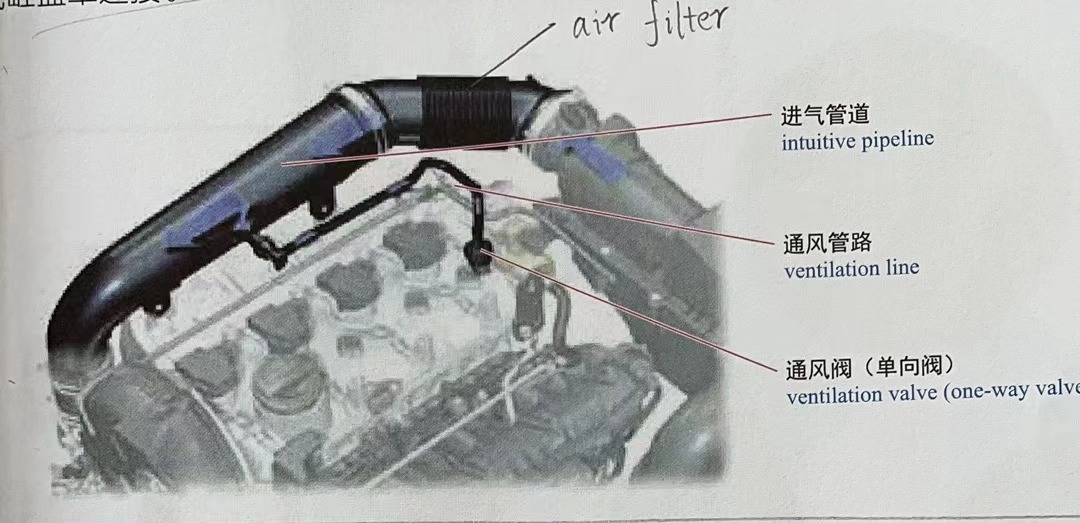
\includegraphics[width=0.7\textwidth]{2-33}
		\end{center}
	\end{block}
\end{frame}
\begin{frame}
	\begin{block}{燃油蒸发控制系统}
		进排气系统的辅助系统
		\begin{center}
			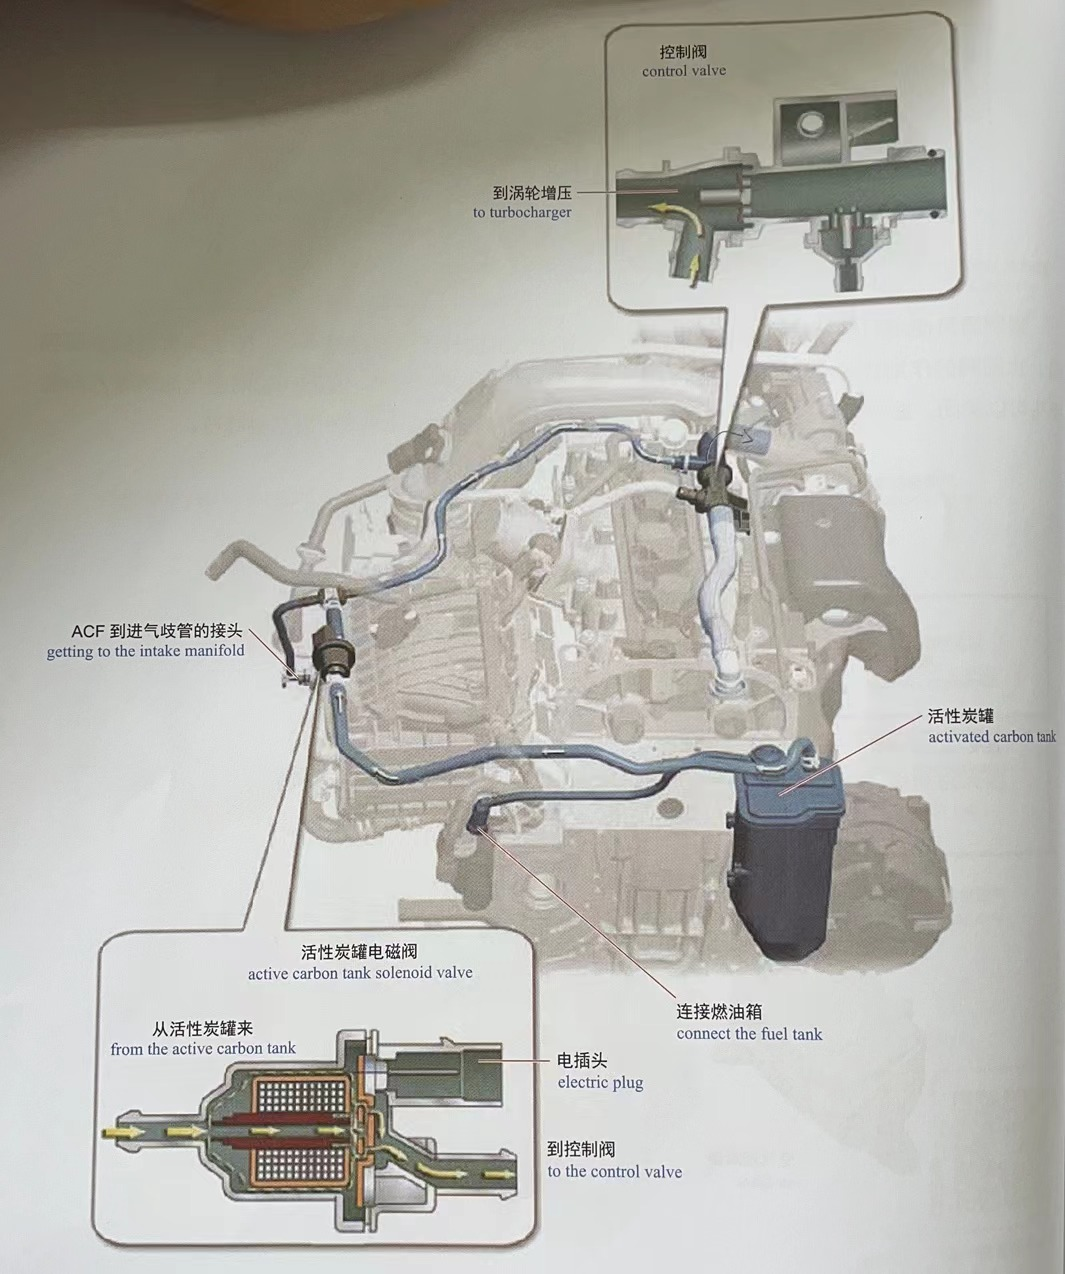
\includegraphics[width=0.5\textwidth]{2-34}
		\end{center}
	\end{block}
\end{frame}
\begin{frame}
	\begin{block}{三元催化转化器TWC(three-way-catalyst)}
		属于排气系统
		\begin{center}
			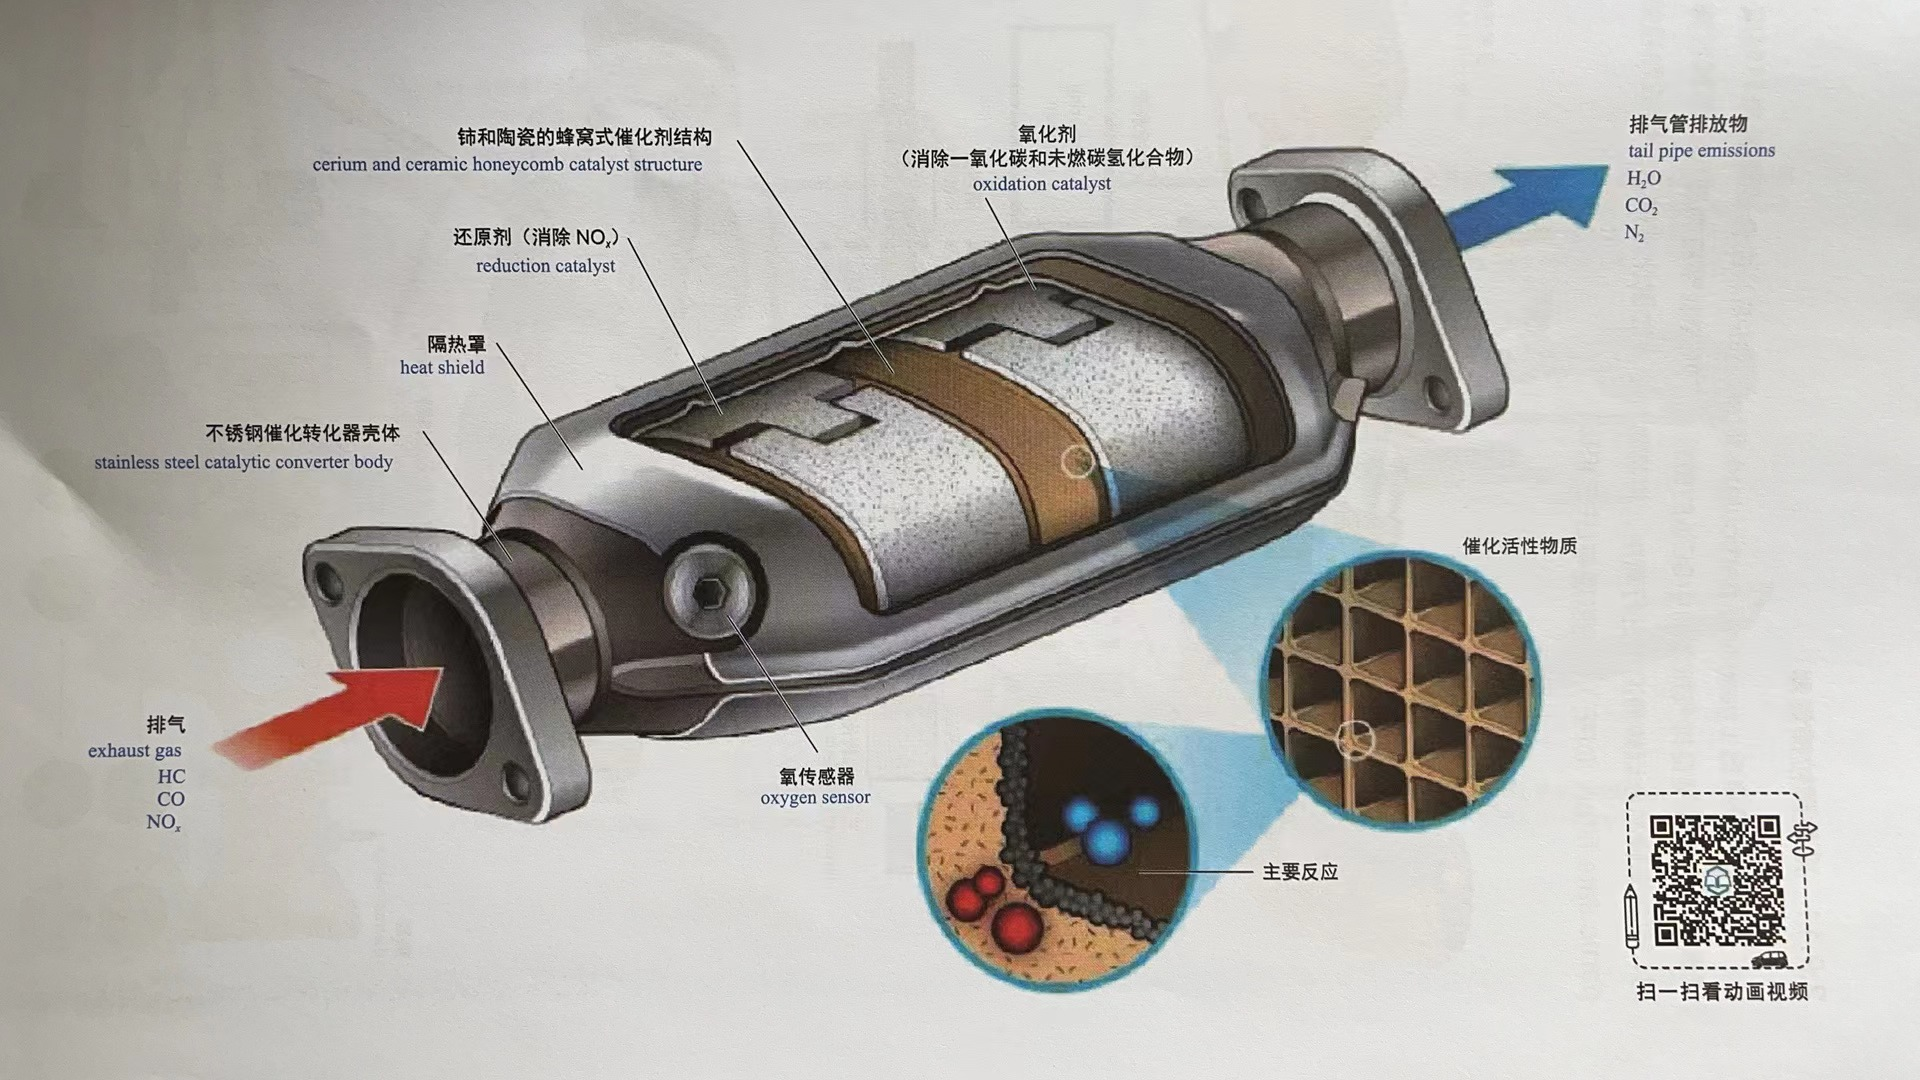
\includegraphics[width=0.7\textwidth]{2-35}
		\end{center}
	\end{block}
\end{frame}
\begin{frame}
	\begin{block}{柴油机后处理系统}
		废气再循环系统的组成部分
		\begin{center}
			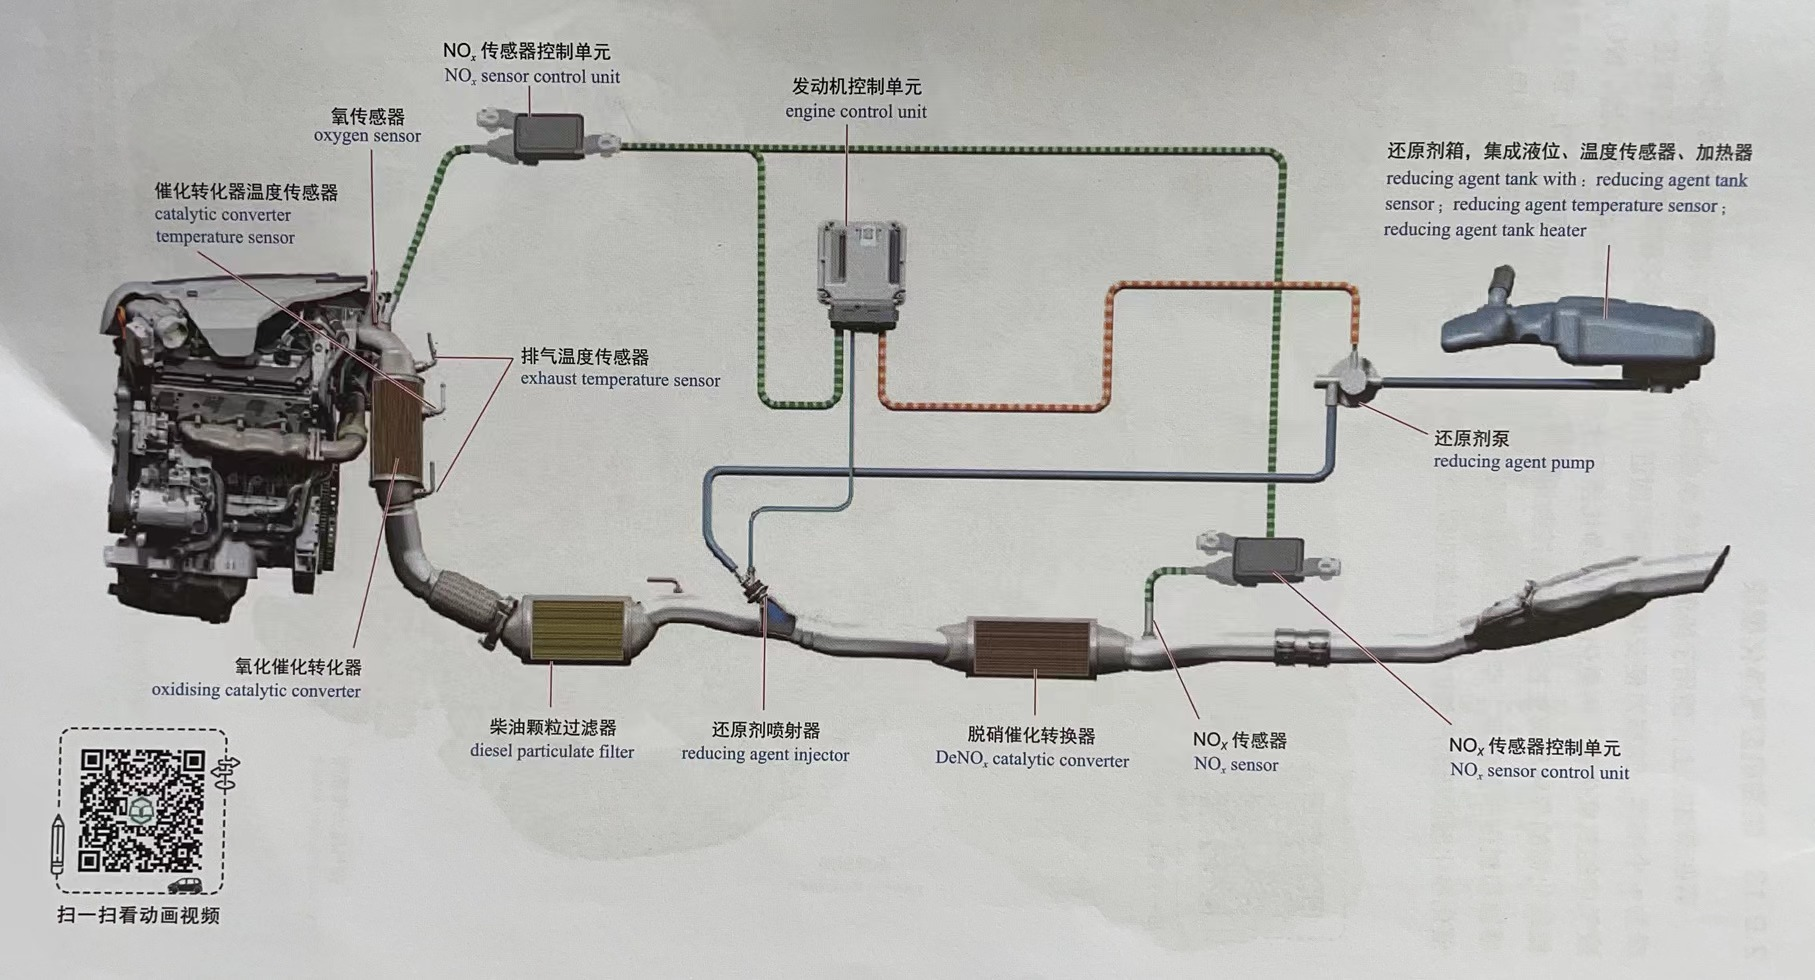
\includegraphics[width=0.7\textwidth]{2-36}
		\end{center}
	\end{block}
\end{frame}
\begin{frame}
	\begin{block}{柴油机废气净化模块}
		\begin{center}
			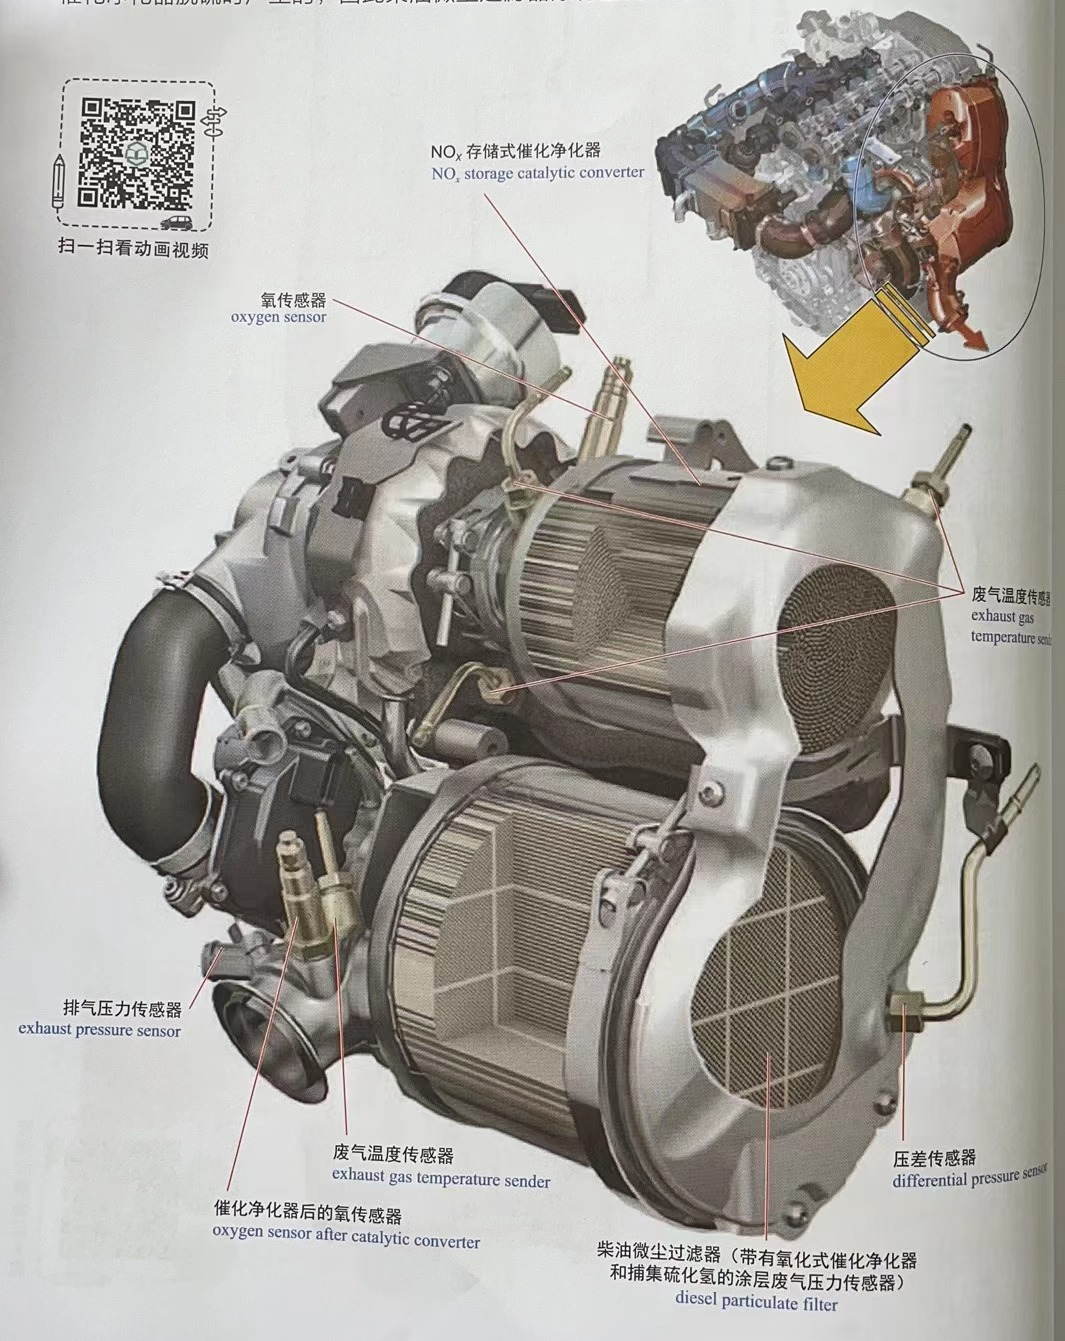
\includegraphics[width=0.5\textwidth]{2-40}
		\end{center}
	\end{block}
\end{frame}
\subsection{润滑系统}
\begin{frame}{润滑系统}
	\begin{block}{润滑油路}
		发动机润滑系统一般采用“压力润滑”,“飞溅润滑”。
	\end{block}
		\begin{block}{机油泵}
		转子式、齿轮式、叶片式
	\end{block}
\end{frame}
\begin{frame}
	\begin{block}{机油滤清器}
		\begin{center}
			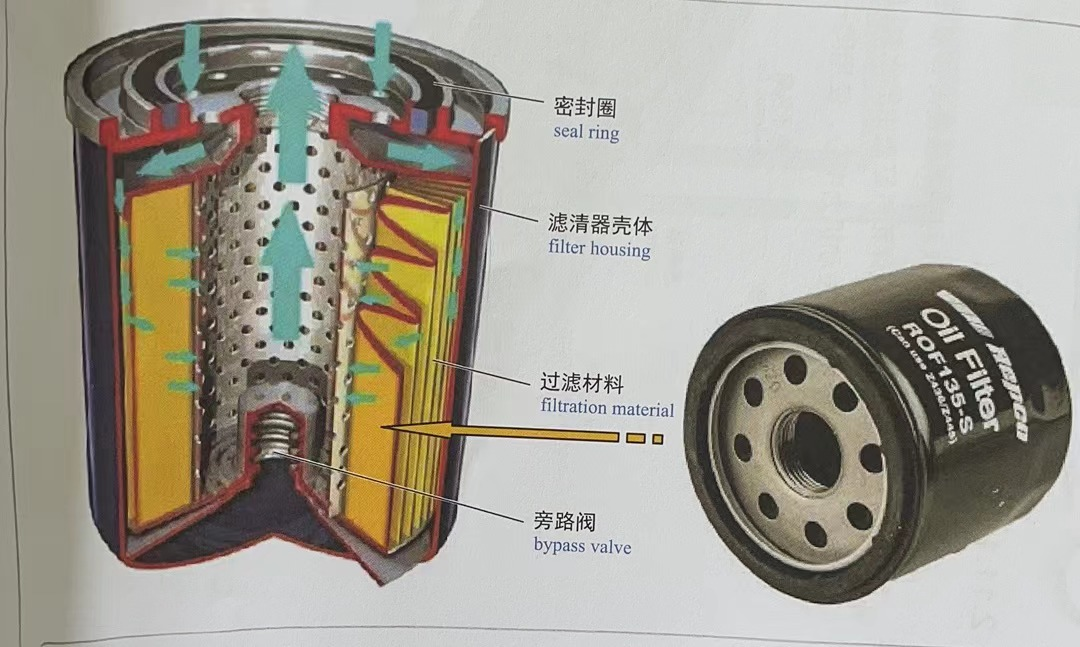
\includegraphics[width=0.7\textwidth]{2-37}
		\end{center}
	\end{block}
\end{frame}
\subsection{冷却系统}
\begin{frame}{冷却系统}
	\begin{block}{节温器}
		在发动机未达到正常工作温度时,使冷却水不经过散热器而是通过旁通水道流回发动机。
	\end{block}
\end{frame}
\begin{frame}
	\begin{block}{电动汽车高压冷却系统}
		\begin{center}
			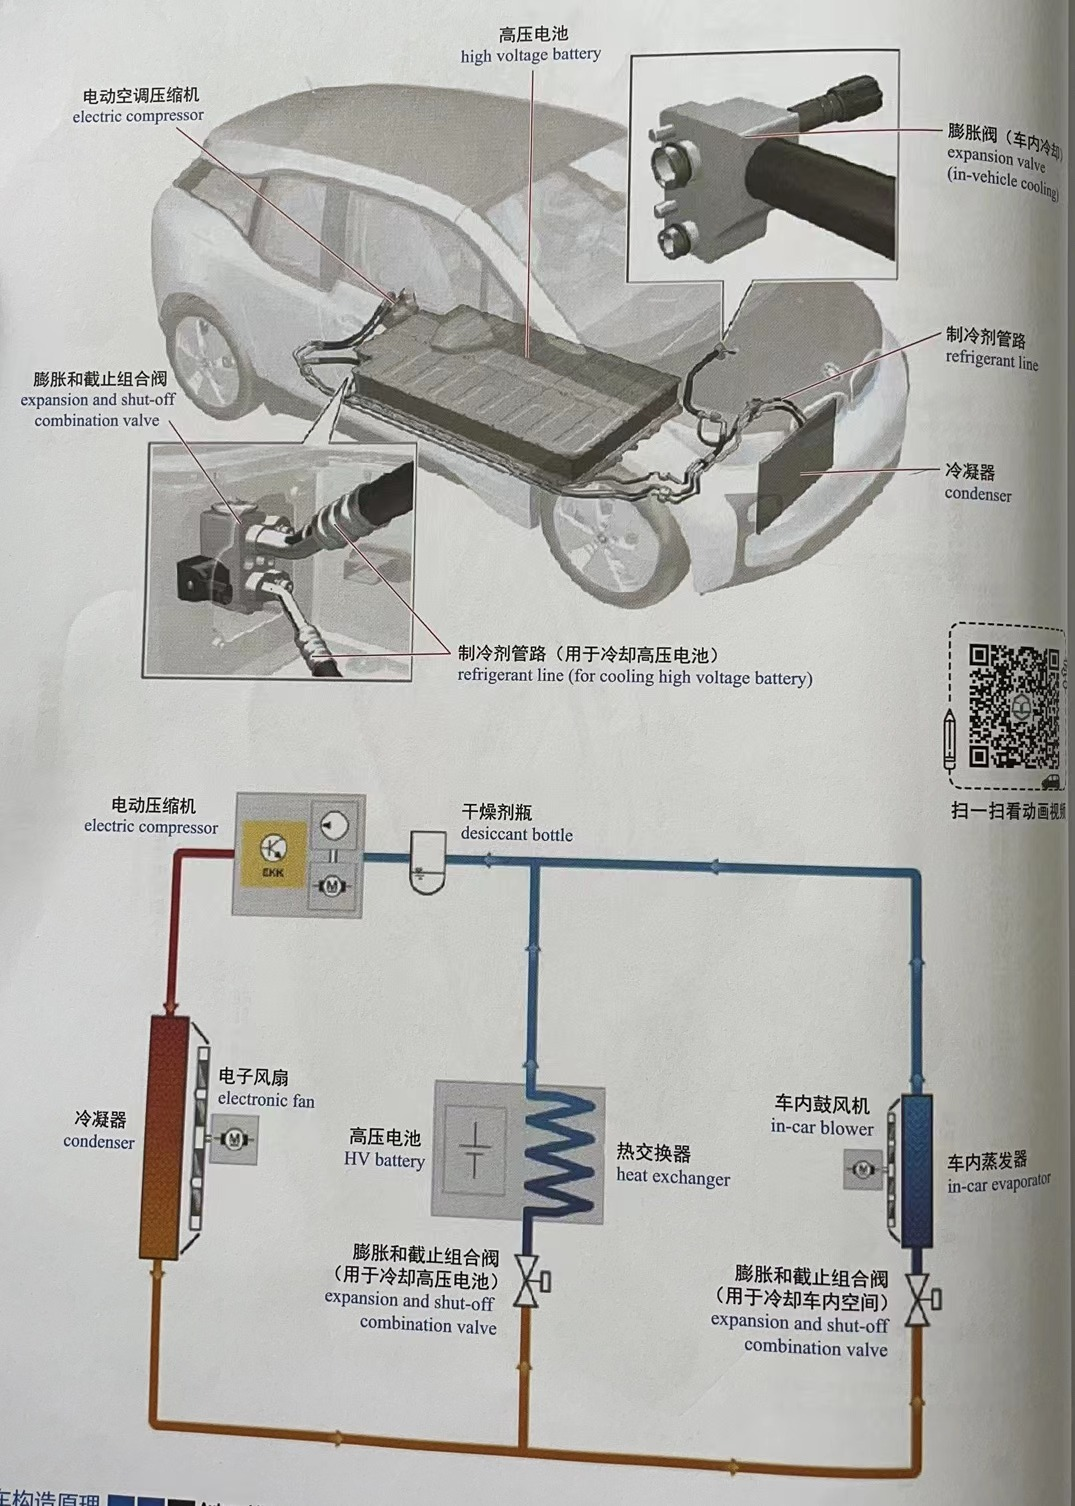
\includegraphics[width=0.5\textwidth]{2-38}
		\end{center}
	\end{block}
\end{frame}
\begin{frame}
	\begin{block}{电驱总成冷却系统}
		\begin{center}
			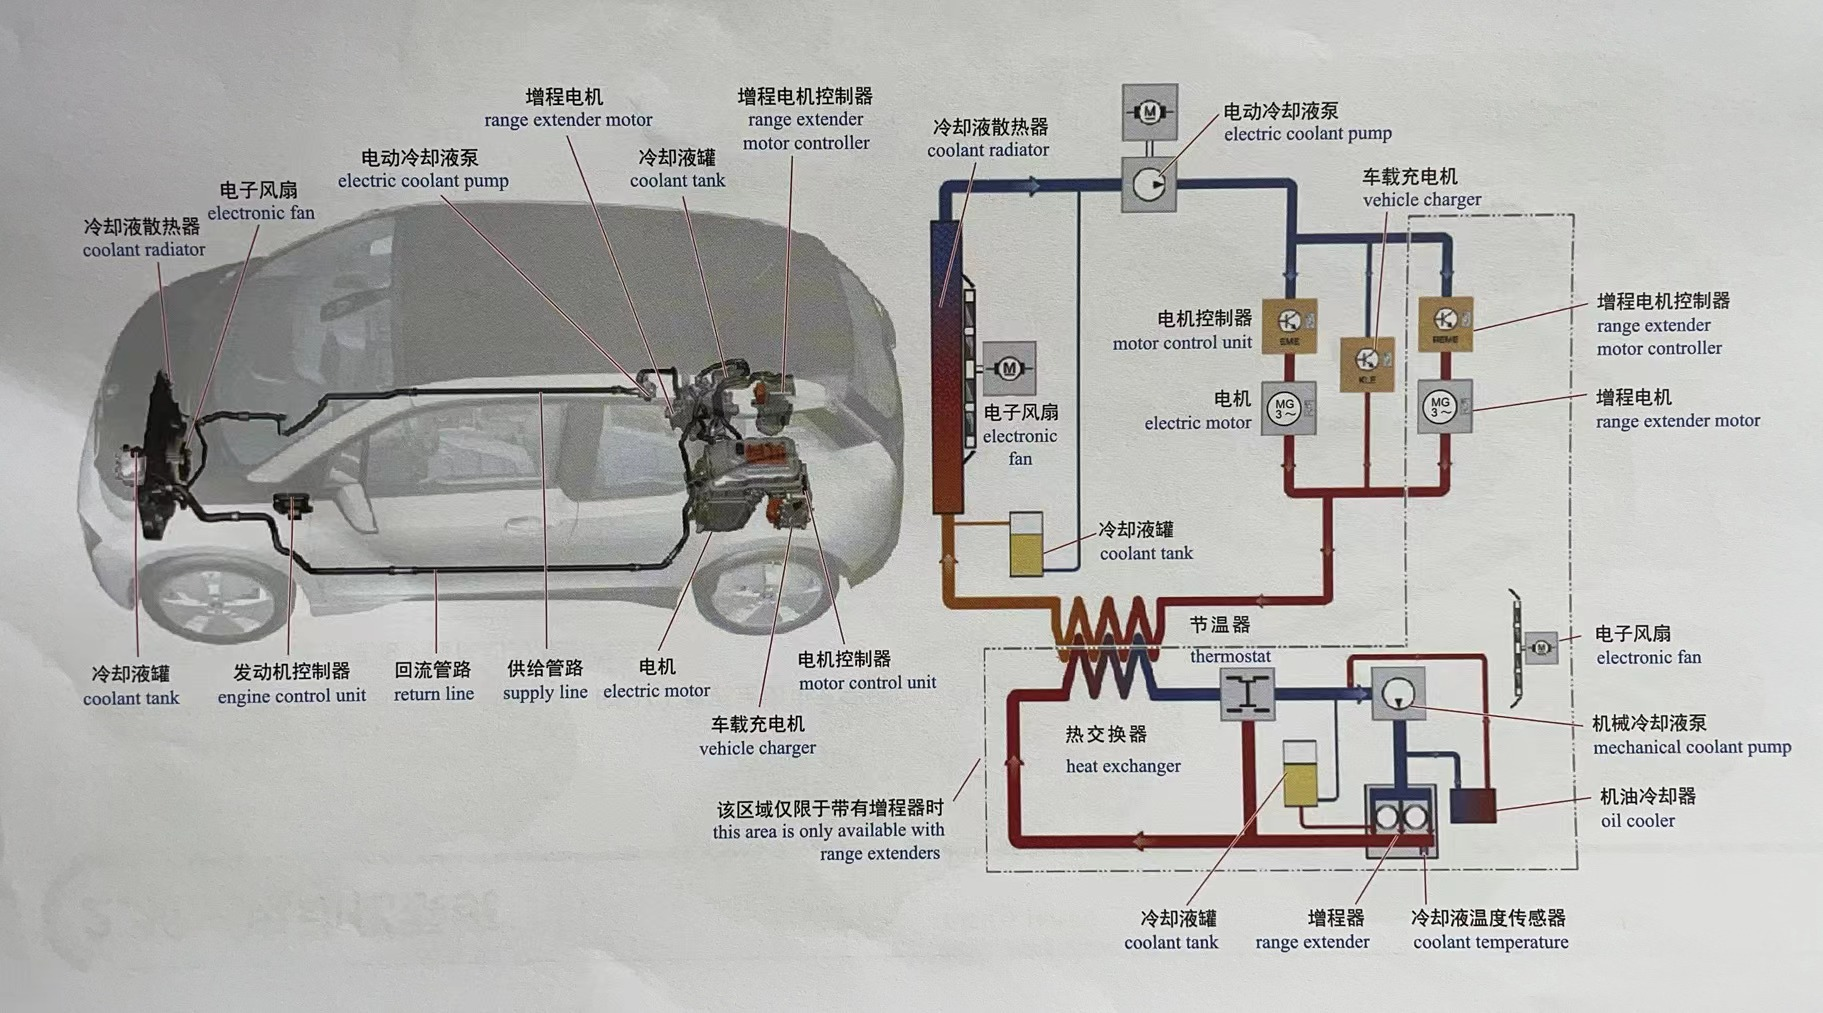
\includegraphics[width=0.9\textwidth]{2-39}
		\end{center}
	\end{block}
\end{frame}
\subsection{电动化系统}
\begin{frame}{电动化系统}
	\begin{block}{纯电动汽车BEV(battery electric vehicle)}
		无发动机
		\begin{center}
			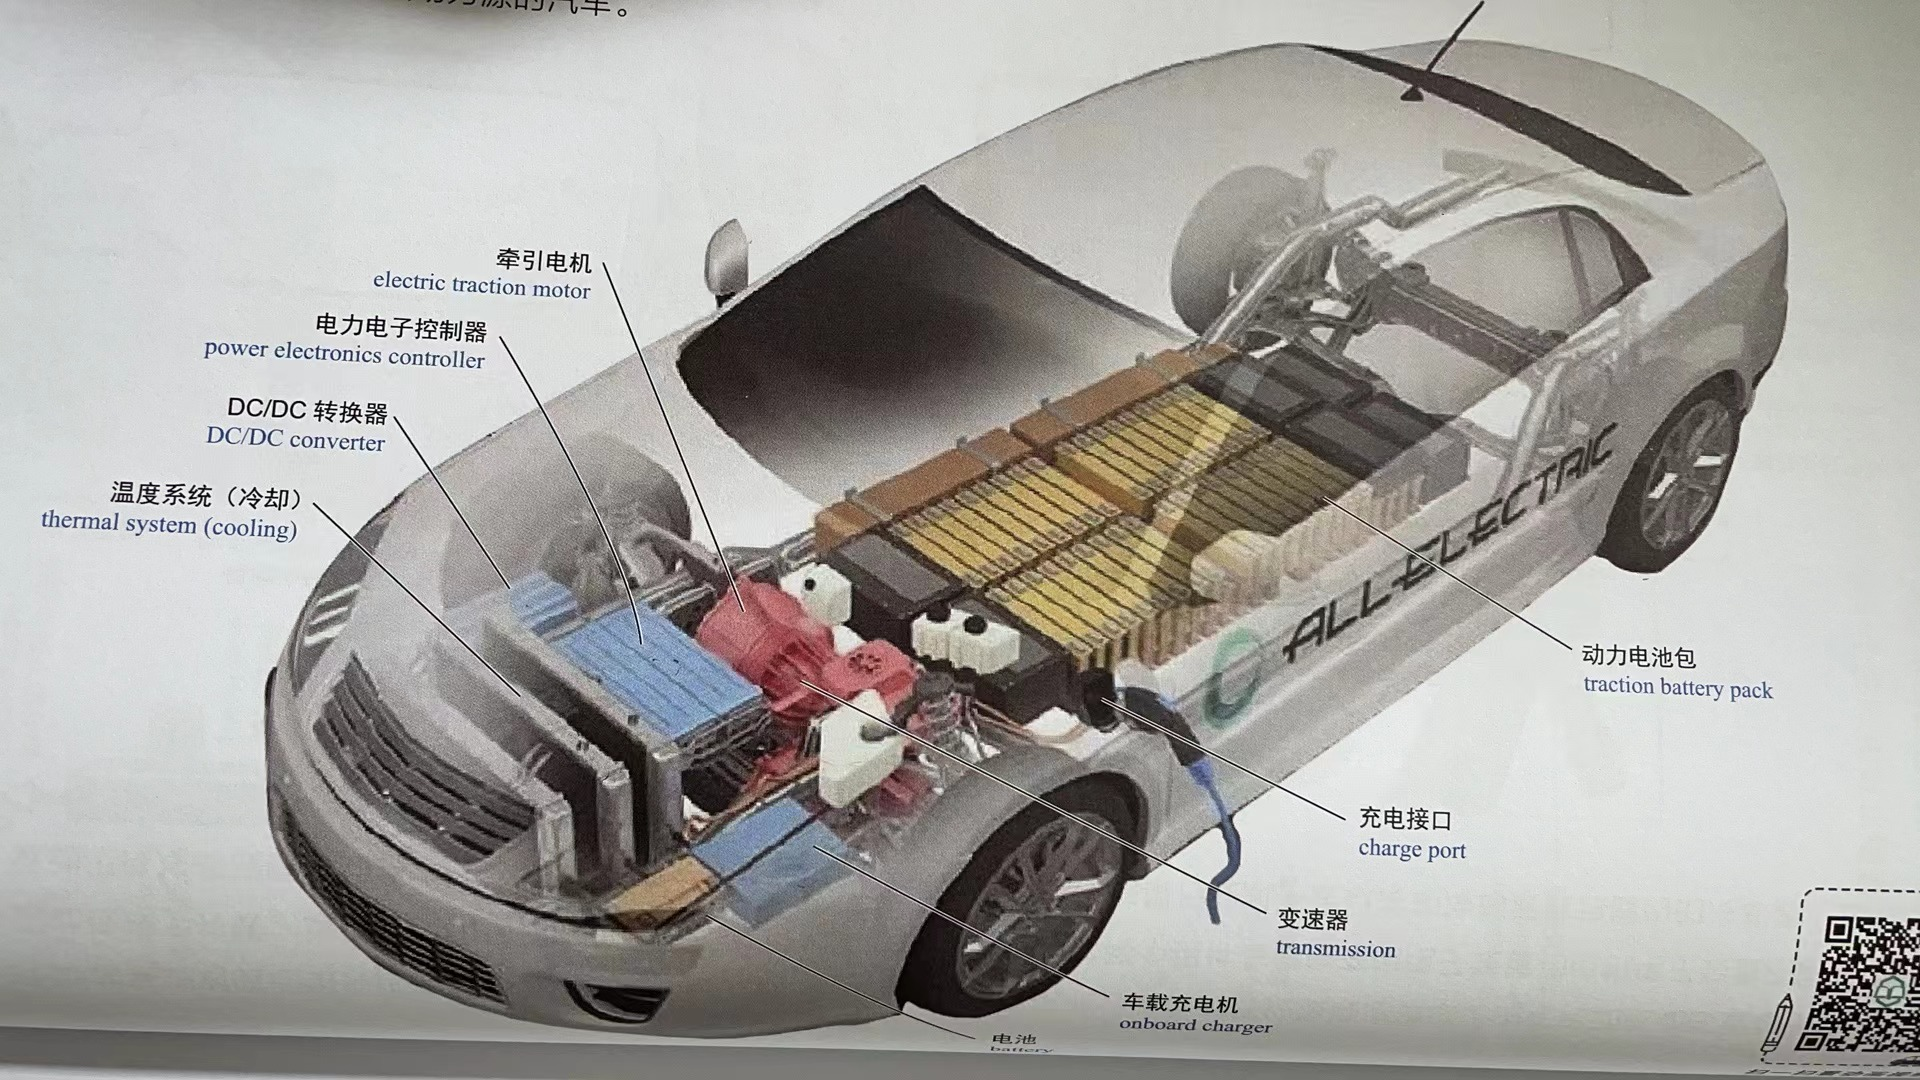
\includegraphics[width=0.5\textwidth]{2-41}
		\end{center}
	\end{block}
\end{frame}
\begin{frame}
	\begin{block}{混合动力汽车}
		\begin{compactitem}
			\item overview
				\begin{equation*}
					\text{混动汽车} \begin{cases}
						\text{If 不能外接充电,油电混动(HEV)} \\
						\parbox{0.7\linewidth}{If 能外插充电,插电混动(PHEV, plug in hybrid electric vehicle)} \\
						\parbox{0.7\linewidth}{发动机作为增程充电器充电而不直接驱动车辆,增程电动REEV}
					\end{cases}
				\end{equation*}
				\begin{equation*}
					\text{HEV} \begin{cases}
						\text{串联混动} \\
						\text{并联混动 PHEV(parallel hybrid electric vehicle)} \\
						\text{混联混动 FHEV(full hybrid electric vehicle)}
					\end{cases}
				\end{equation*}
		\end{compactitem}
	\end{block}
\end{frame}
\begin{frame}
	\begin{block}{}
		\begin{compactitem}
			\item  REEV
				\begin{center}
					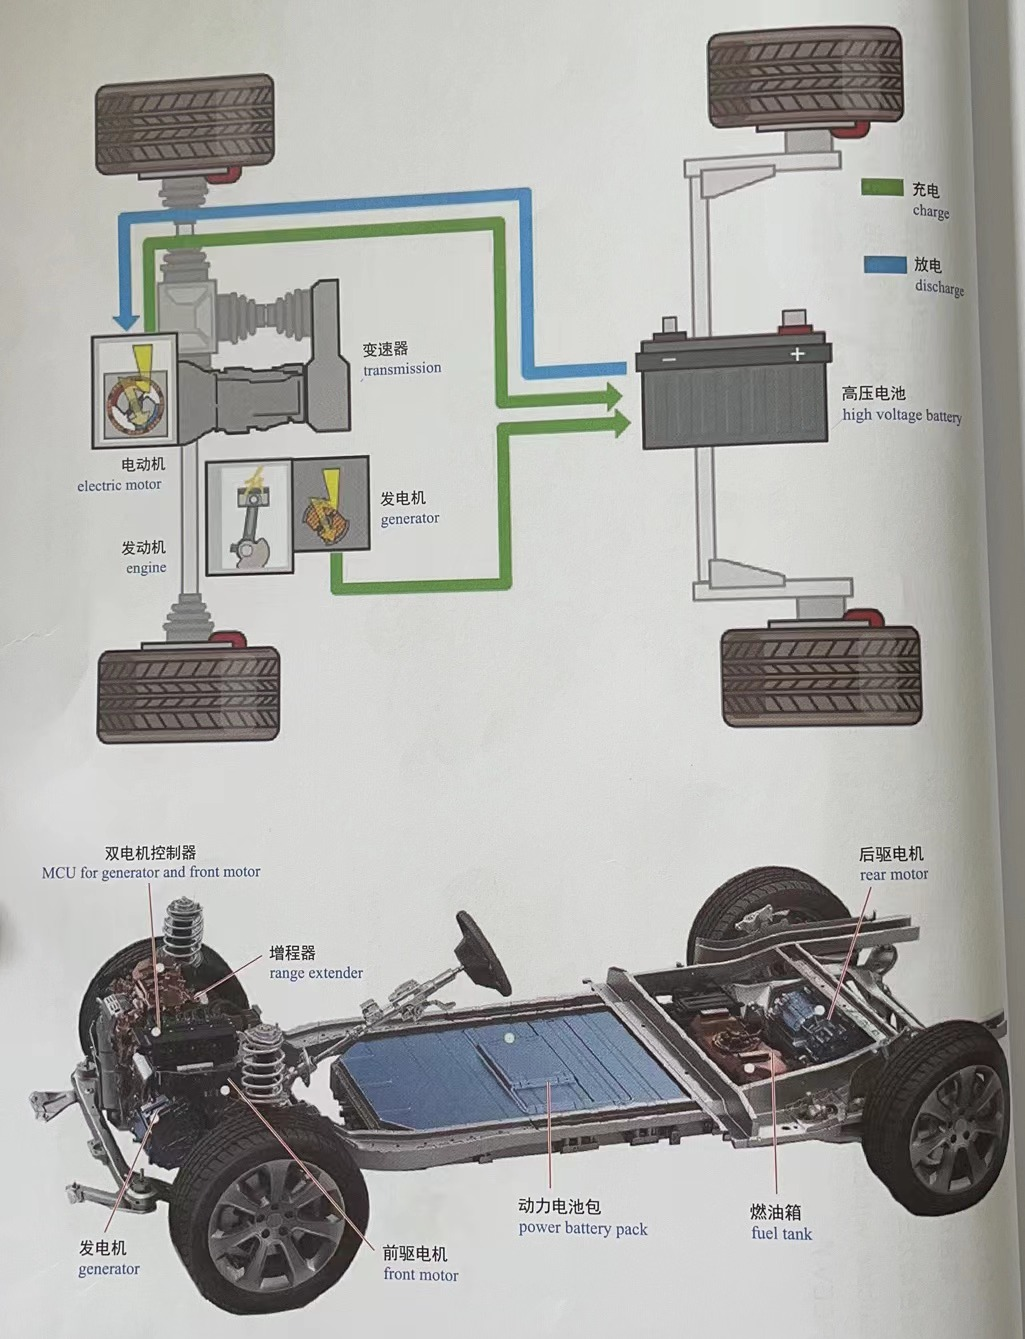
\includegraphics[width=0.5\textwidth]{2-42}
				\end{center}
		\end{compactitem}
	\end{block}
\end{frame}
\begin{frame}
	\begin{block}{}
		\begin{compactitem}
			\item  PHEV
			\begin{center}
				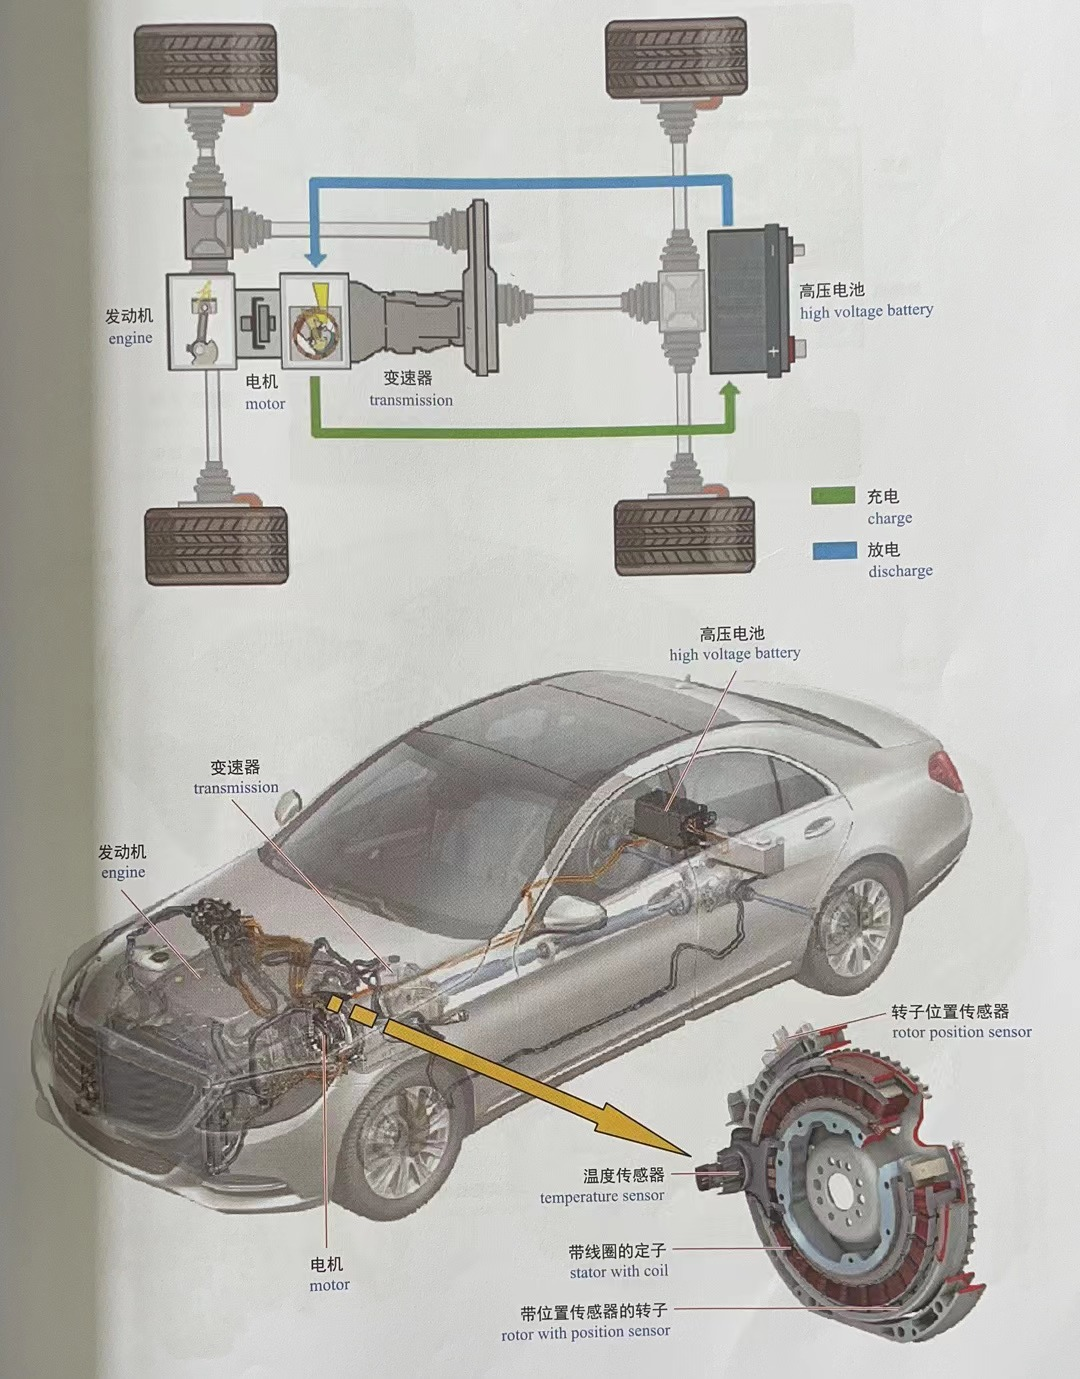
\includegraphics[width=0.5\textwidth]{2-43}
			\end{center}
		\end{compactitem}
	\end{block}
\end{frame}
\begin{frame}
	\begin{block}{}
		\begin{compactitem}
			\item  CHEV 混联式混合动力汽车
			
			工作模式:串联混动 or 并联混动
			\begin{center}
				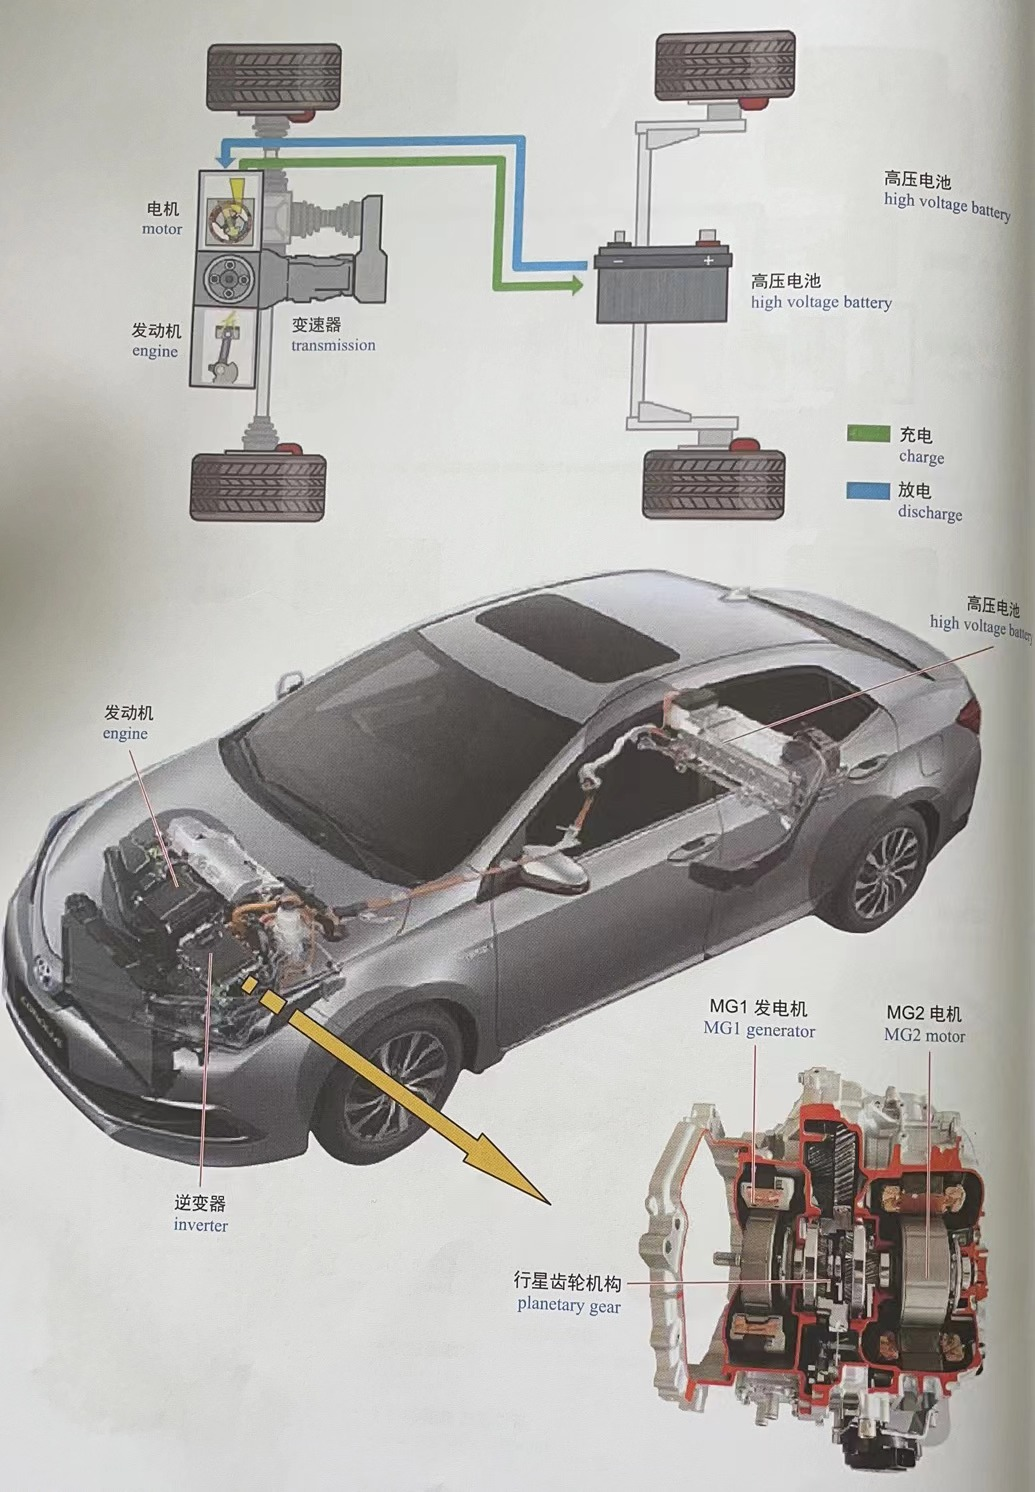
\includegraphics[width=0.5\textwidth]{2-44}
			\end{center}
		\end{compactitem}
	\end{block}
\end{frame}
\begin{frame}
	\begin{block}{}
		\begin{compactitem}
			\item  MHEV(mild hybrid electric vehicle)轻度混动
			\begin{center}
				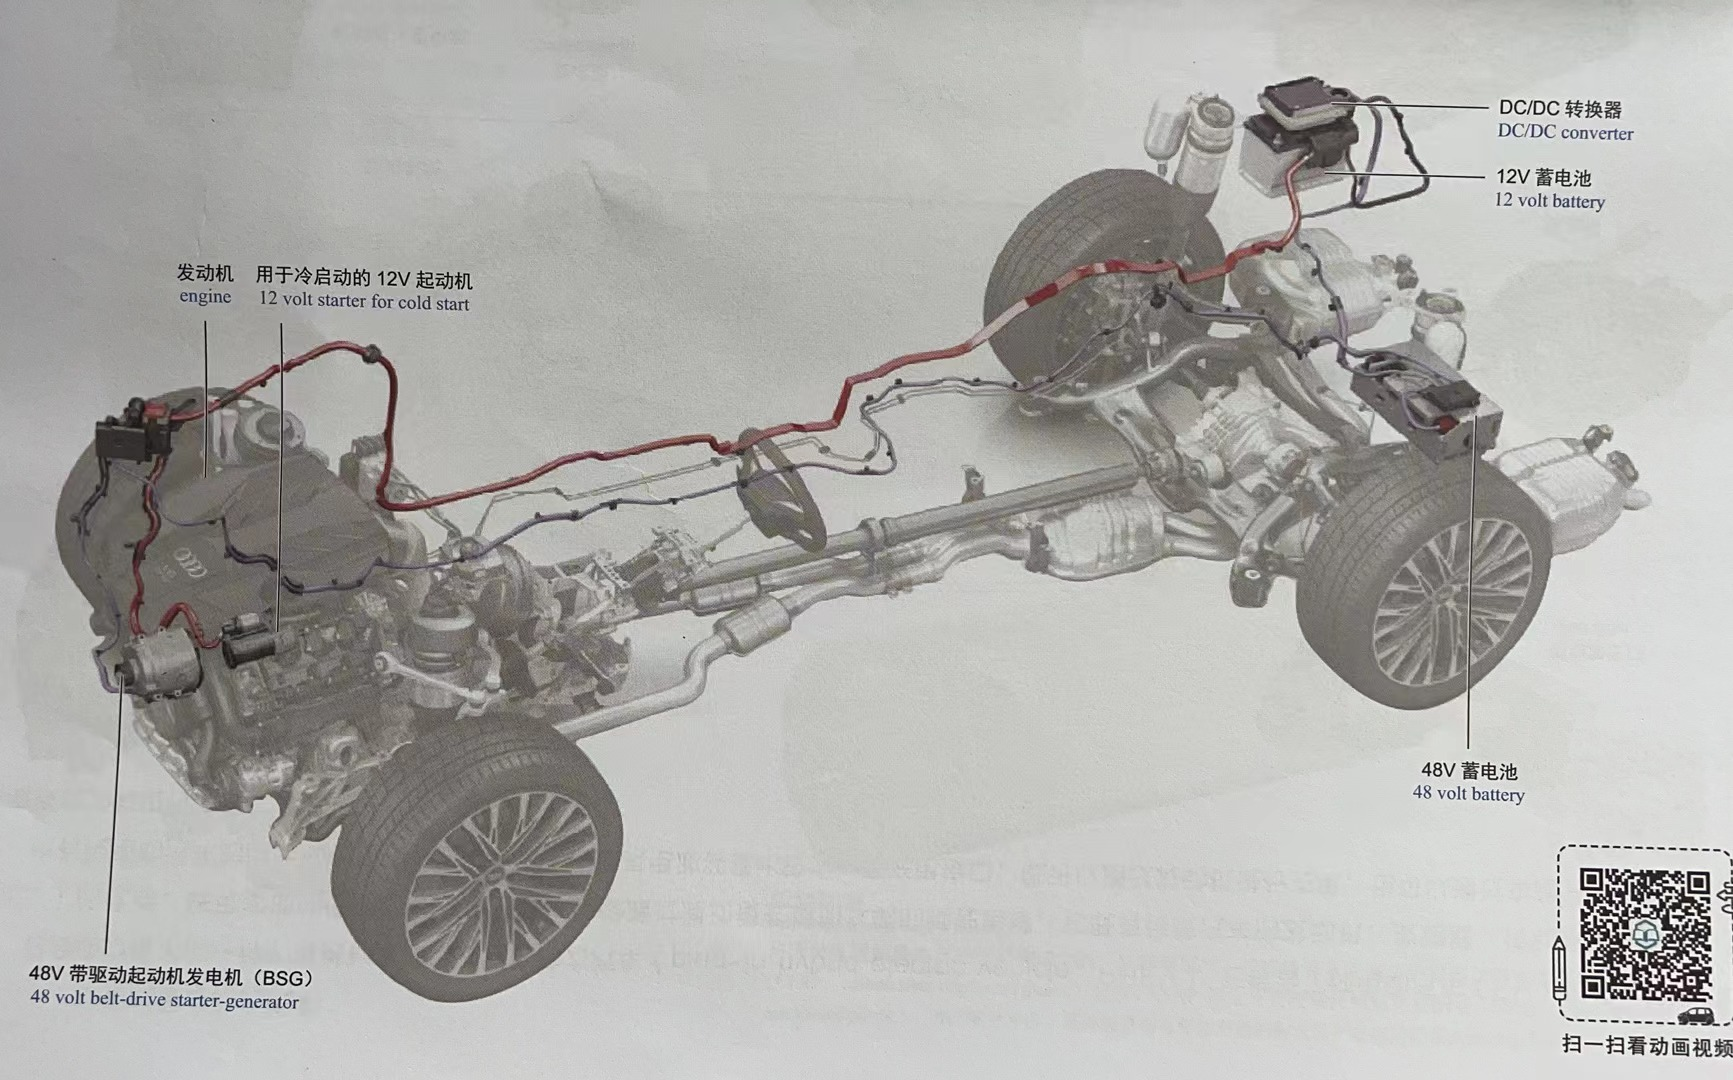
\includegraphics[width=0.7\textwidth]{2-45}
			\end{center}
		\end{compactitem}
	\end{block}
\end{frame}
\begin{frame}
	\begin{block}{}
		\begin{compactitem}
			\item  PHEV插电式混合动力汽车
			\begin{center}
				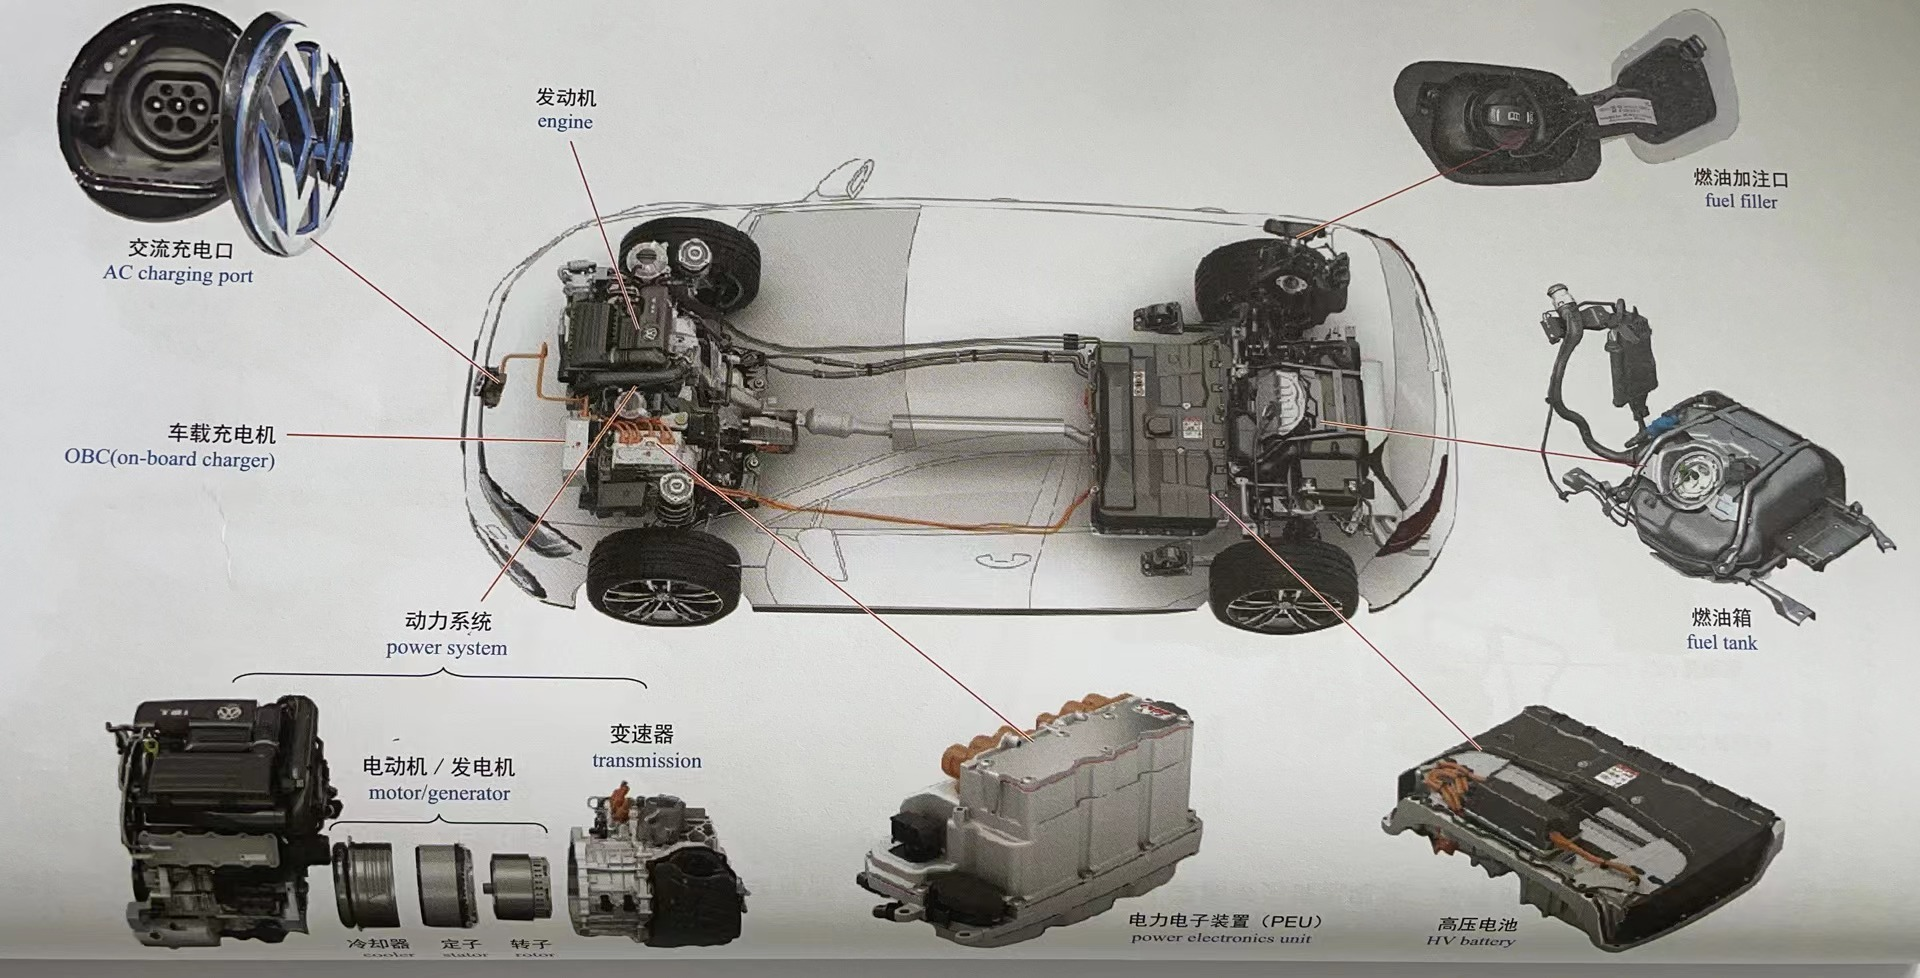
\includegraphics[width=0.9\textwidth]{2-46}
			\end{center}
		\end{compactitem}
	\end{block}
\end{frame}
\begin{frame}
	\begin{block}{}
		\begin{compactitem}
			\item  氢燃料电池汽车
			
			main power source is electricity, which 由氢气制成 in the 氢燃料电池
		\end{compactitem}
	\end{block}
\end{frame}
\begin{frame}
	\begin{block}{动力电池}
		\begin{compactitem}
			\item 三元锂电池 tenery lithinum battery 最常用
			\begin{center}
				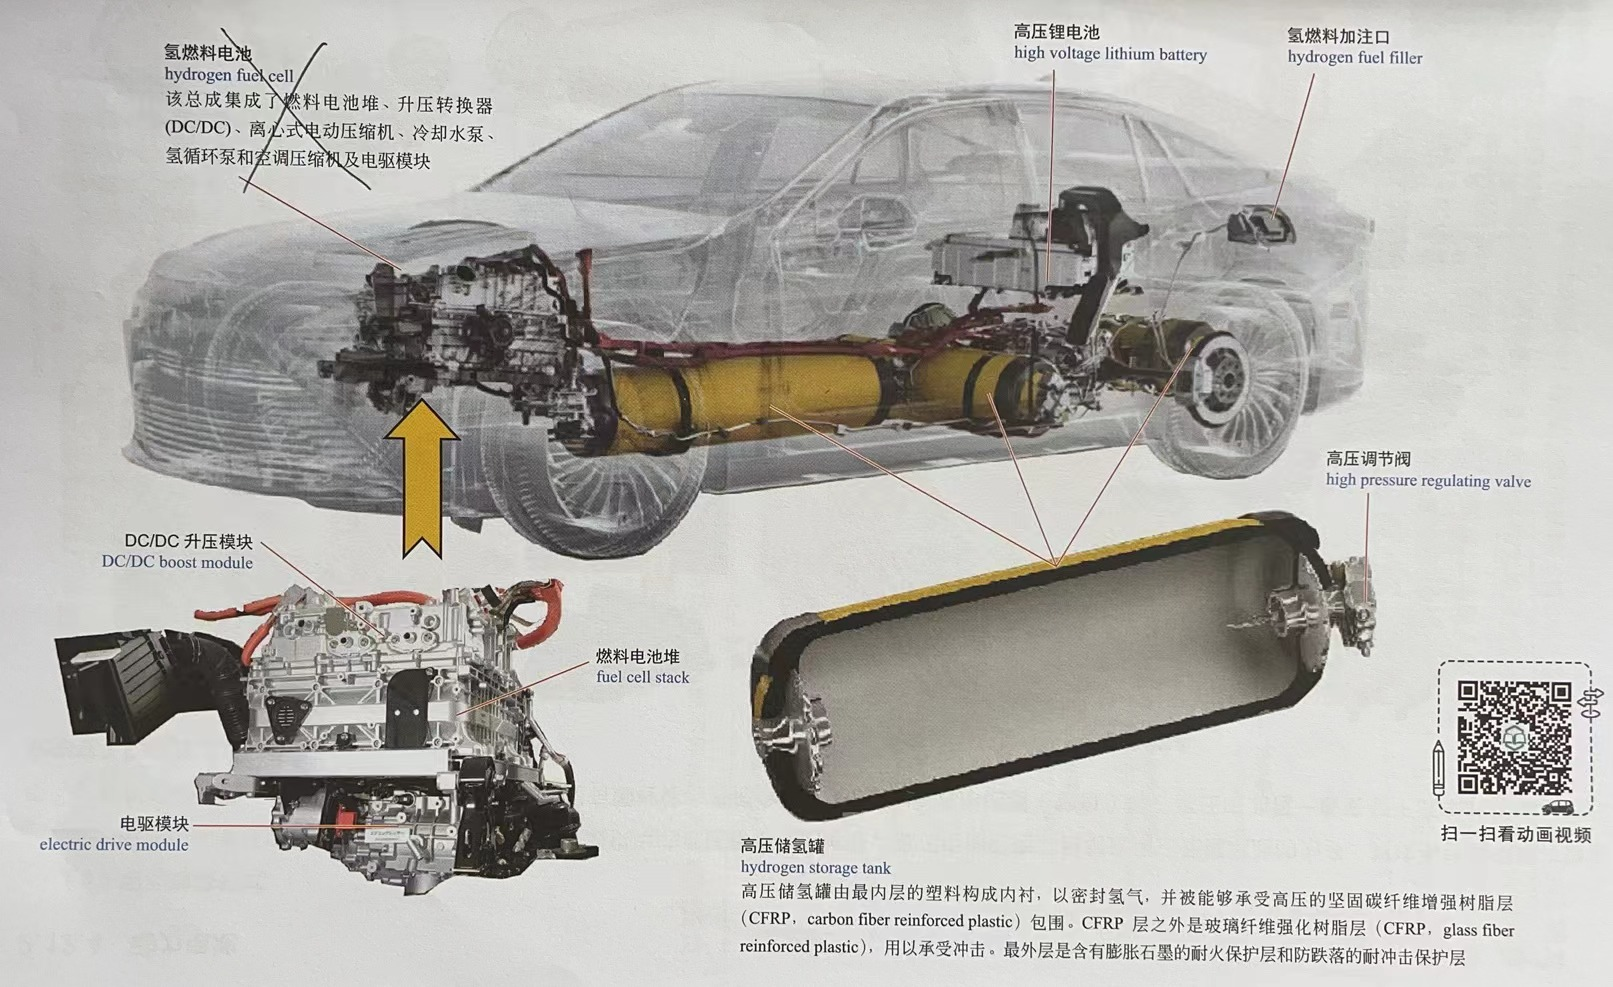
\includegraphics[width=0.7\textwidth]{2-47}
			\end{center}
		\end{compactitem}
	\end{block}
\end{frame}
\begin{frame}
	\begin{block}{}
		\begin{compactitem}
			\item 磷酸铁锂电池
			\begin{center}
				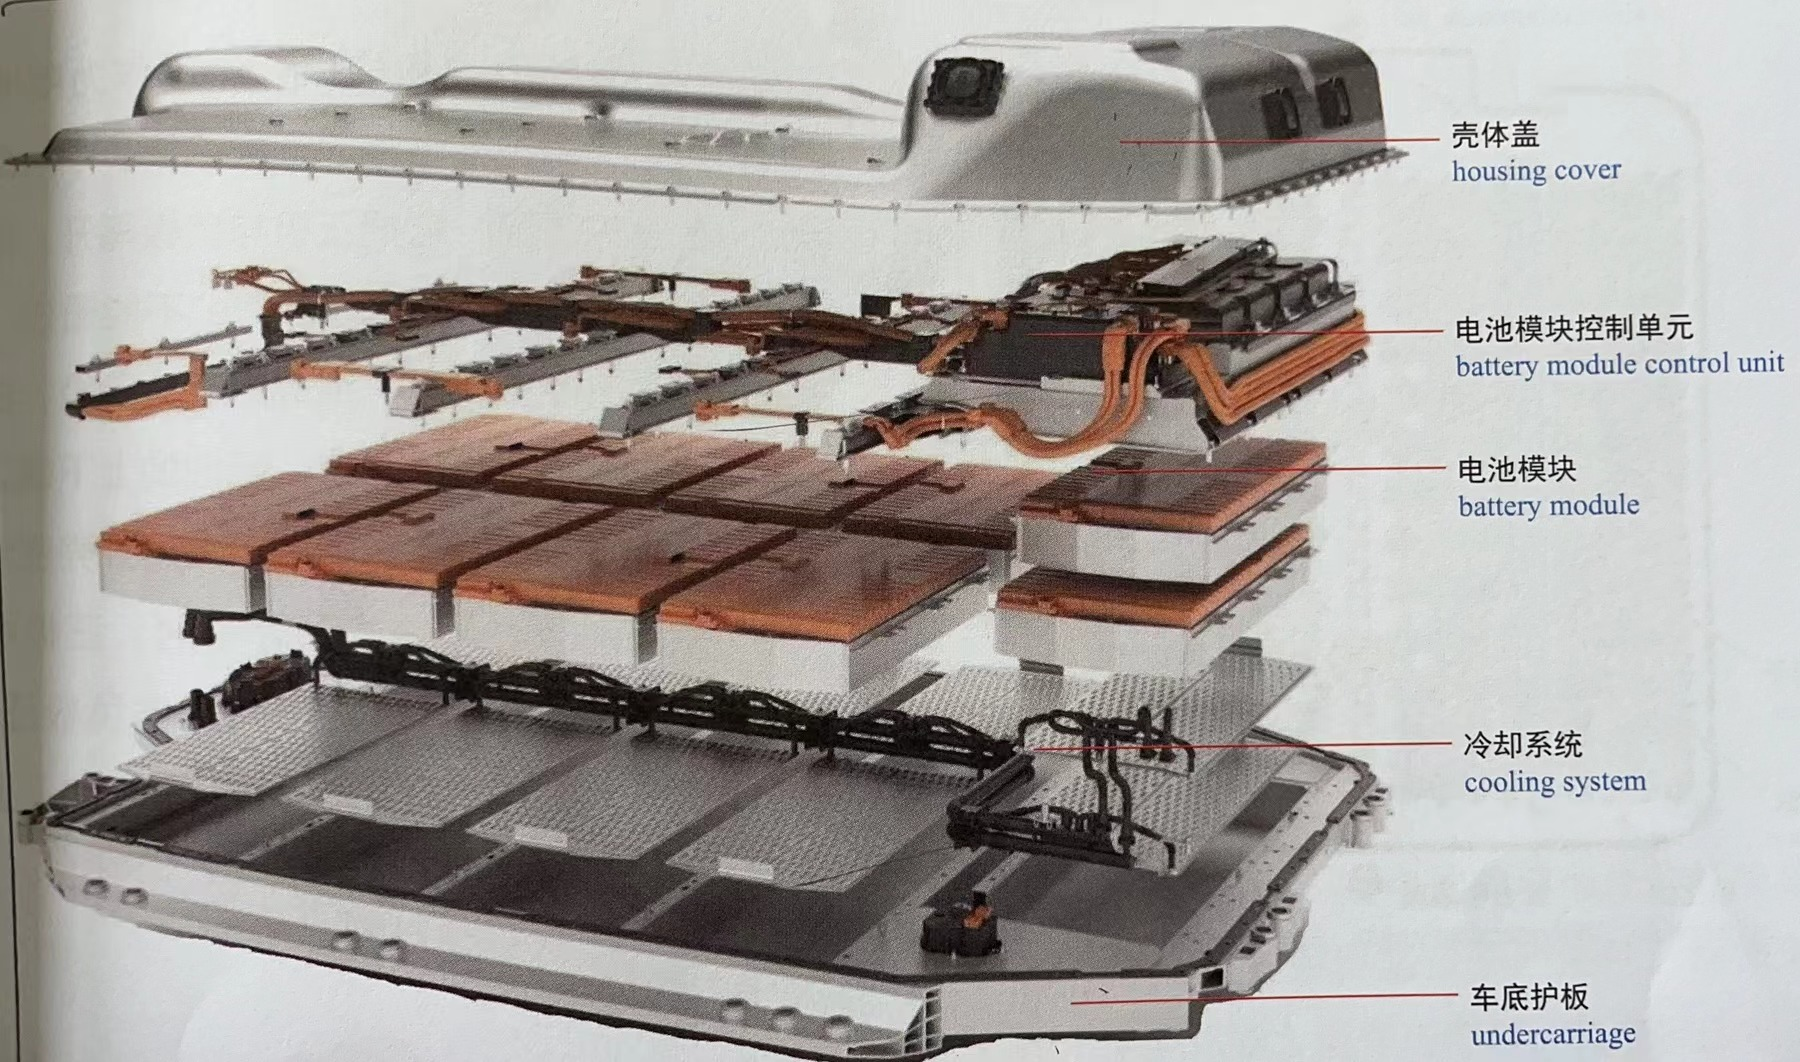
\includegraphics[width=0.7\textwidth]{2-48}
			\end{center}
		\end{compactitem}
	\end{block}
\end{frame}
\begin{frame}
	\begin{block}{}
		\begin{compactitem}
			\item 镍氢电池
			\begin{center}
				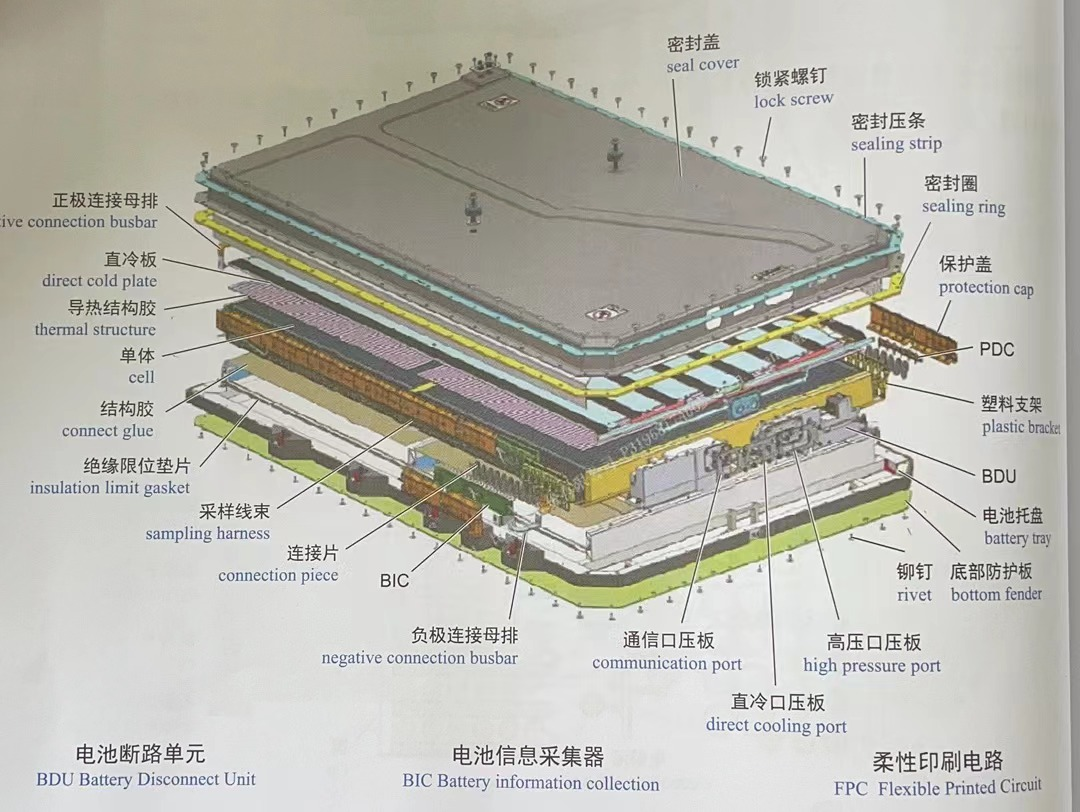
\includegraphics[width=0.7\textwidth]{2-49}
			\end{center}
			\item 氢燃料电池
		\end{compactitem}
	\end{block}
\end{frame}
\begin{frame}
	\begin{block}{高压充电}
		\begin{compactitem}
			\item 慢充 and 快充
				\begin{compactenum}
					\item 慢充 = 交流充电:
					
						AC 充电桩/壁挂式充电盒/家用供电插座$\Rightarrow$ AC 充电口 $\Rightarrow \underset{\parbox{0.3\linewidth}{\centering \tiny 交流电转直流电}}{\text{\underline{高压电控总成}}}$ $\Rightarrow$ power battery
					\item 快充 = 直流充电:
					
						充电柜 $\Rightarrow$ DC charging port $\Rightarrow$ power battery
				\end{compactenum}
			\item on-board charger车载充电机
				
				动态调整充电I/V based on the data provided by BMS to complete charging process
		\end{compactitem}
	\end{block}
\end{frame}
\begin{frame}
	\begin{figure}[htbp]
		\centering
		\caption*{车载充电机}
		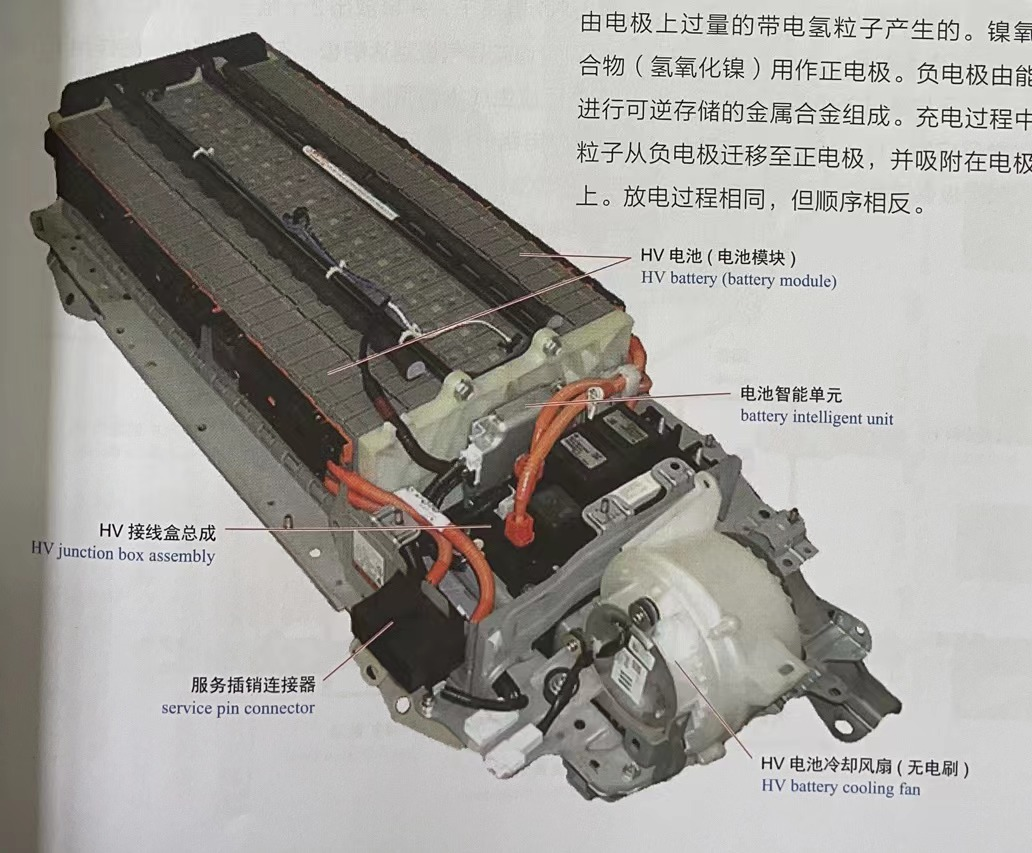
\includegraphics[width=0.7\textwidth]{2-50}
	\end{figure}
\end{frame}
\begin{frame}
	\begin{block}{电驱系统}
		\begin{compactitem}
			\item overview of 电驱系统
			\begin{center}
				\includegraphics[width=0.7\textwidth]{2-51}
			\end{center}
		\end{compactitem}
	\end{block}
\end{frame}
\begin{frame}
	\begin{block}{}
		\begin{compactitem}
			\item 电机类型
				\begin{compactenum}
					\item 永磁同步电机(PMSM permanent magnet synchronous motor): 转子转速 = 定子磁场转速
					\item 三相交流异步电机(感应电机):转子转速!=定子磁场转速
				\end{compactenum}
		\end{compactitem}
						\begin{figure}[htbp]
		\centering
		\subfloat[PMSM]{\centering  \includegraphics[width=0.45\textwidth]{2-52}}
		\subfloat[三相交流异步电机]{\centering  \includegraphics[width=0.45\textwidth]{2-52}}
	\end{figure}
	\end{block}
\end{frame}
\begin{frame}
	\begin{compactitem}
		\item 电力电子单元 PEU : also known as N合一电控总成
	\end{compactitem}
\end{frame}
\begin{frame}
	\begin{block}{VCU整车控制器}
		\begin{compactitem}
			\item 是新能源汽车的核心部件
			\item 主要功能:
			
				解析驾驶员需求、监控汽车行驶状态,协调控制单元(BMC, MCU, EMS(energy management syste),TCU(transmission control unit)),实现整车上下电、驱动控制、能量回收、附件控制、故障诊断等功能
		\end{compactitem}
	\end{block}
\end{frame}
\end{document}